\chapter{The Large Hadron Collider and CMS}~\label{ch:CMSExperiment}

{\small \rightline{“It doesn't matter how beautiful your theory is, it doesn't matter }
\vspace{-2ex}
\rightline{how smart you are. If it doesn't agree with experiment, it's wrong.”}
\rightline{-Richard Feynman}}
\vspace{4ex}

In this chapter, we discuss the experimental setup. First, in Sec~\ref{sec:LHC} we discuss the accelerator complex that accelerates protons into counter-rotating beams which are then collided to produce the two-photon events which are collected by the CMS detector~\ref{sec:CMSDetector}. 

\section{The Large Hadron Collider}~\label{sec:LHC}
\begin{figure}[!htb]
	\centering
	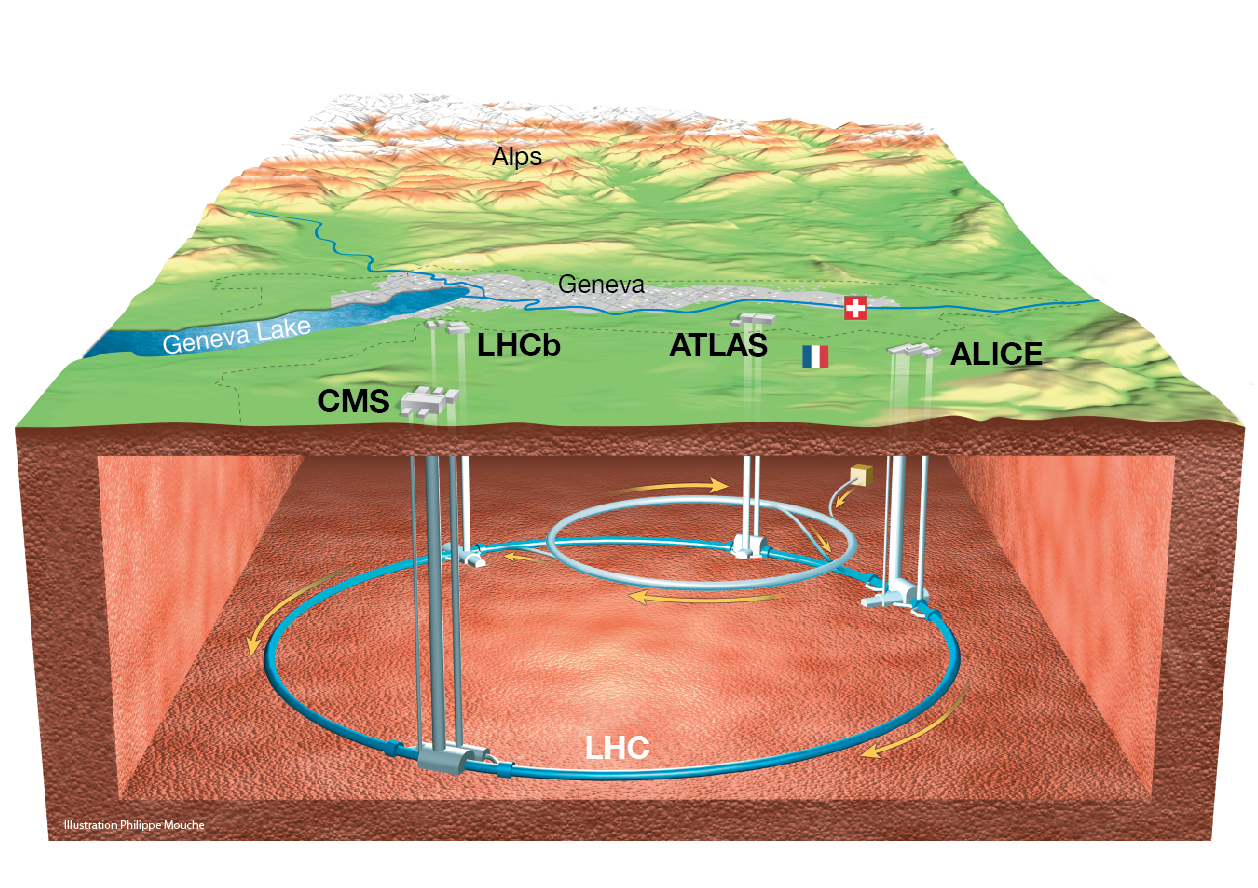
\includegraphics[scale=0.3]{fig/lhc_overview.png}
	\caption{An overview of the location of LHC and its four interaction points~\cite{Mouche:1708847}.}
	\label{lhc-overview}
\end{figure}


% \RaggedRight \parindent=25pt
\justifying \parindent=25pt


The Large Hadron Collider (LHC) depicted in Figure~\ref{lhc-overview}, is the world's largest and most powerful man-made particle accelerator as of date. It is nestled approximately 100 meters underground, beneath the Jura Mountains and Lac Leman, straddling Geneva, Switzerland and the neighbouring territory of France.

The LHC was built as a general purpose collider and the data it produces serve various physics programs from precision measurements in the Standard Model to searches for exotic, beyond standard model physics. In this section, we will briefly describe the LHC accelerator complex, the engineering motivations for the collider design and the key physics performance in various runs.

\subsubsection{LHC Ring of Magnets}
The full 27-km LHC ring is made up of segments of cryogenically-cooled superconducting dipole and quadrupole magnets that house two counter-rotating proton beam pipes. The dipole magnets steer the particle beams into an approximately circular orbit. Superconducting quadrupole magnets focus the particle beams while higher order moment magnets are used for beam corrections, all in the effort to maximize collision rates~\cite{Rossi:2002ye}. A total of 1248 dipole and 400 quadrupole magnets constitute the full ring, each of them 15-m and 3-m in length respectively. They are constructed with niobium-titanium (NbTi) which produce an operational field strength of 7.7 T. To maintain their superconductive state, they are cooled to 1.9 K with liquid helium.

\subsubsection{Experiments Overview}
 
 Protons are sourced from a bottle of hydrogen and end their journey when they collide at four interaction points in the LHC (see Figure~\ref{fig:accelerator_complex}). Around these interaction points are the four main experiments: ATLAS \cite{ATLAS:2008xda}, CMS \cite{CMS:2008xjf}, LHCb \cite{LHCb:2008vvz}, and ALICE \cite{ALICE:2008ngc}. ATLAS (A Toroidal LHC Apparatus) and CMS (Compact Muon Solenoid) are two of the general-purpose detectors that have similar physics programs where their results are often benchmarked against each other's. ALICE (A Large Ion Collider Experiment), focuses on heavy ion collisions and primarily studies the quark-gluon plasma. LHCb specializes on studying CP violation, or the investigating slight differences in matter and antimatter using ``beauty" quark decays. Four additional, auxiliary experiments also operate through these points, TOTEM, LHCf, MoEDAL and FASER.  

\subsubsection{The CERN Accelerator Complex}

Before the protons or lead ions reach the collision points, they first have to go through a series of accelerators shown in Figure~\ref{fig:accelerator_complex} to reach the desired total collision energy of 13 TeV for Run II. For the sake of brevity, we will only consider proton beams at this point but lead ions follow the same route but start from vaporized led. Protons, on the other hand, are sourced from molecular hydrogen which are ionized. Ionized hydrogen (H-) are then extracted and injected to Linac4 where Radiofrequency (RF) cavitites are used to accelerate them to 160 MeV. They are then prepared to enter the first of the circular accelerators called the Proton Synchrotron Booster (PSB). Before they enter the PSB, the ions are stripped of their electrons and the protons are accelerated to 2 GeV. This prepares them for injection to the Proton Synchrotron (PS) which increases the beam energy to 26 GeV. The final step before injection to the LHC is in the Super Proton Synchrotron where the beams are accelerated up to 450 GeV. 

% This means that the counter-rotating particle beams each have an energy of E = 6.5 TeV \cite{LHCpop}

Once the proton beams are transferred into the two counter-rotating beam pipes of the LHC, it takes around 20 minutes for the protons to reach their maximum energy of 6.5 TeV. The beams can circulate for many hours inside the LHC beam pipes under normal operating conditions and during collisions, they meet at at the interaction points inside the four detectors described earlier. 


% \begin{figure}[!htbp]
% 	\centering
% 	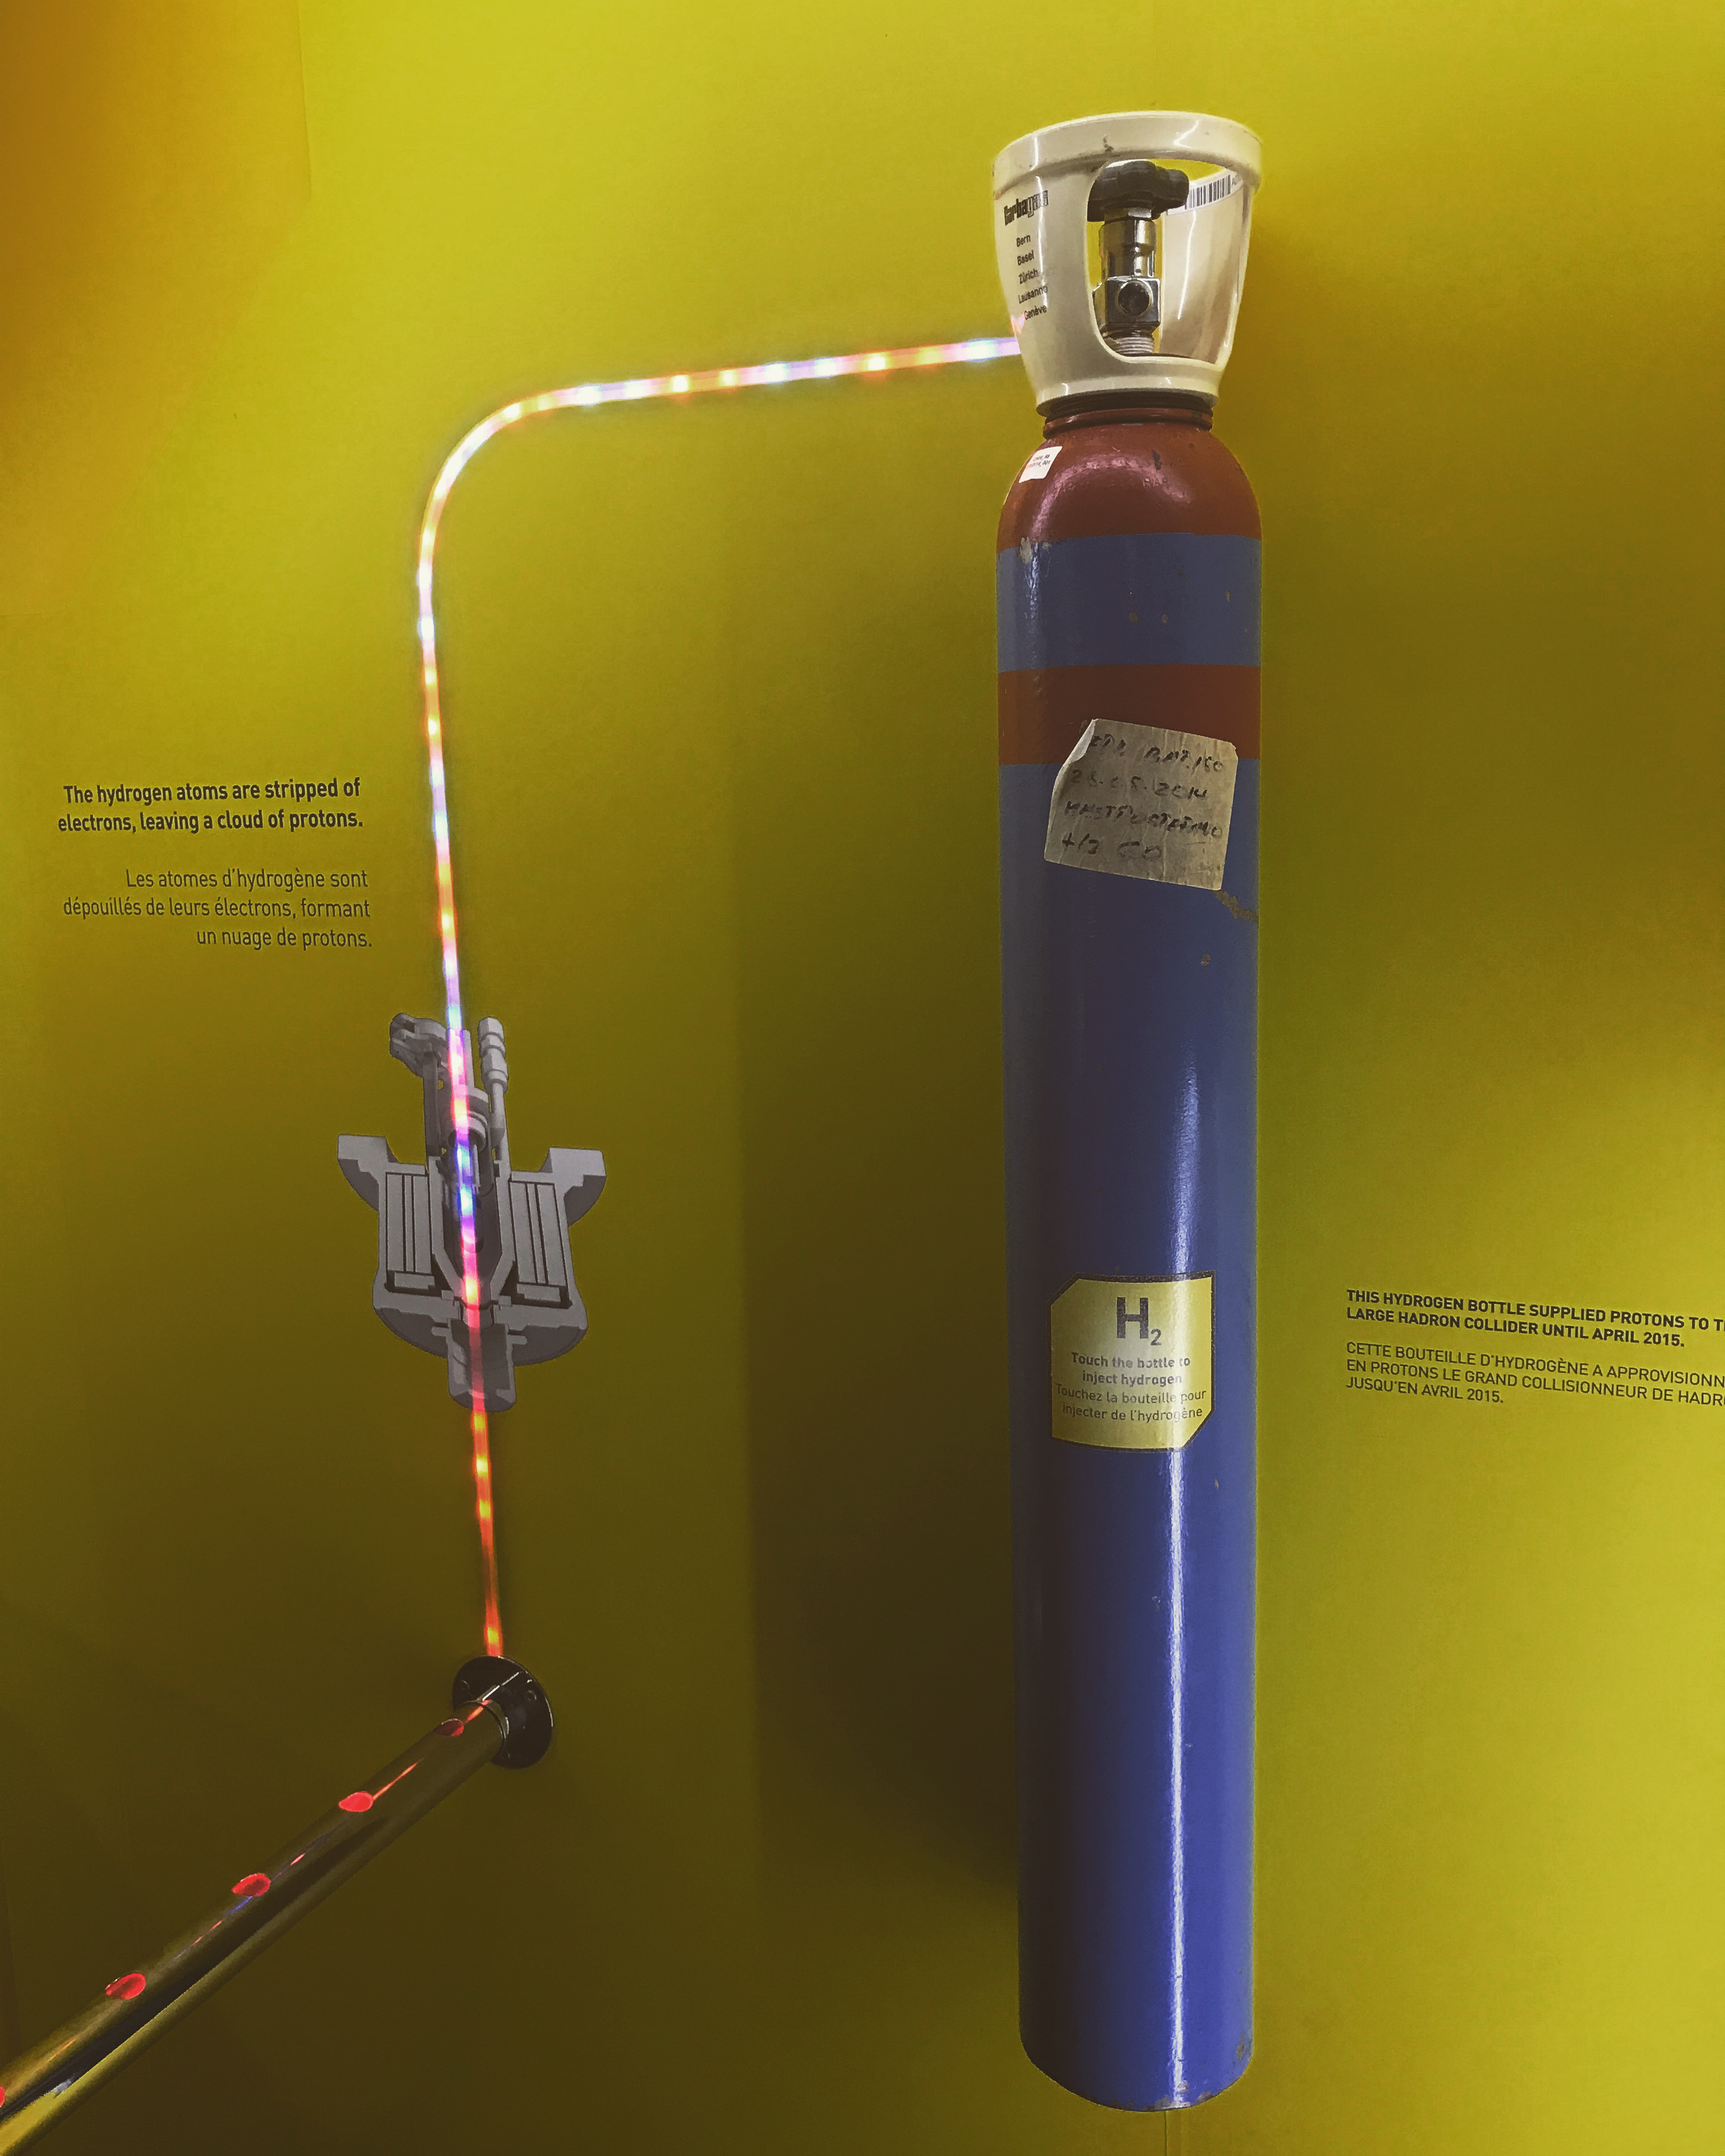
\includegraphics[scale=0.038]{fig/H2Bottle.JPG}
% 	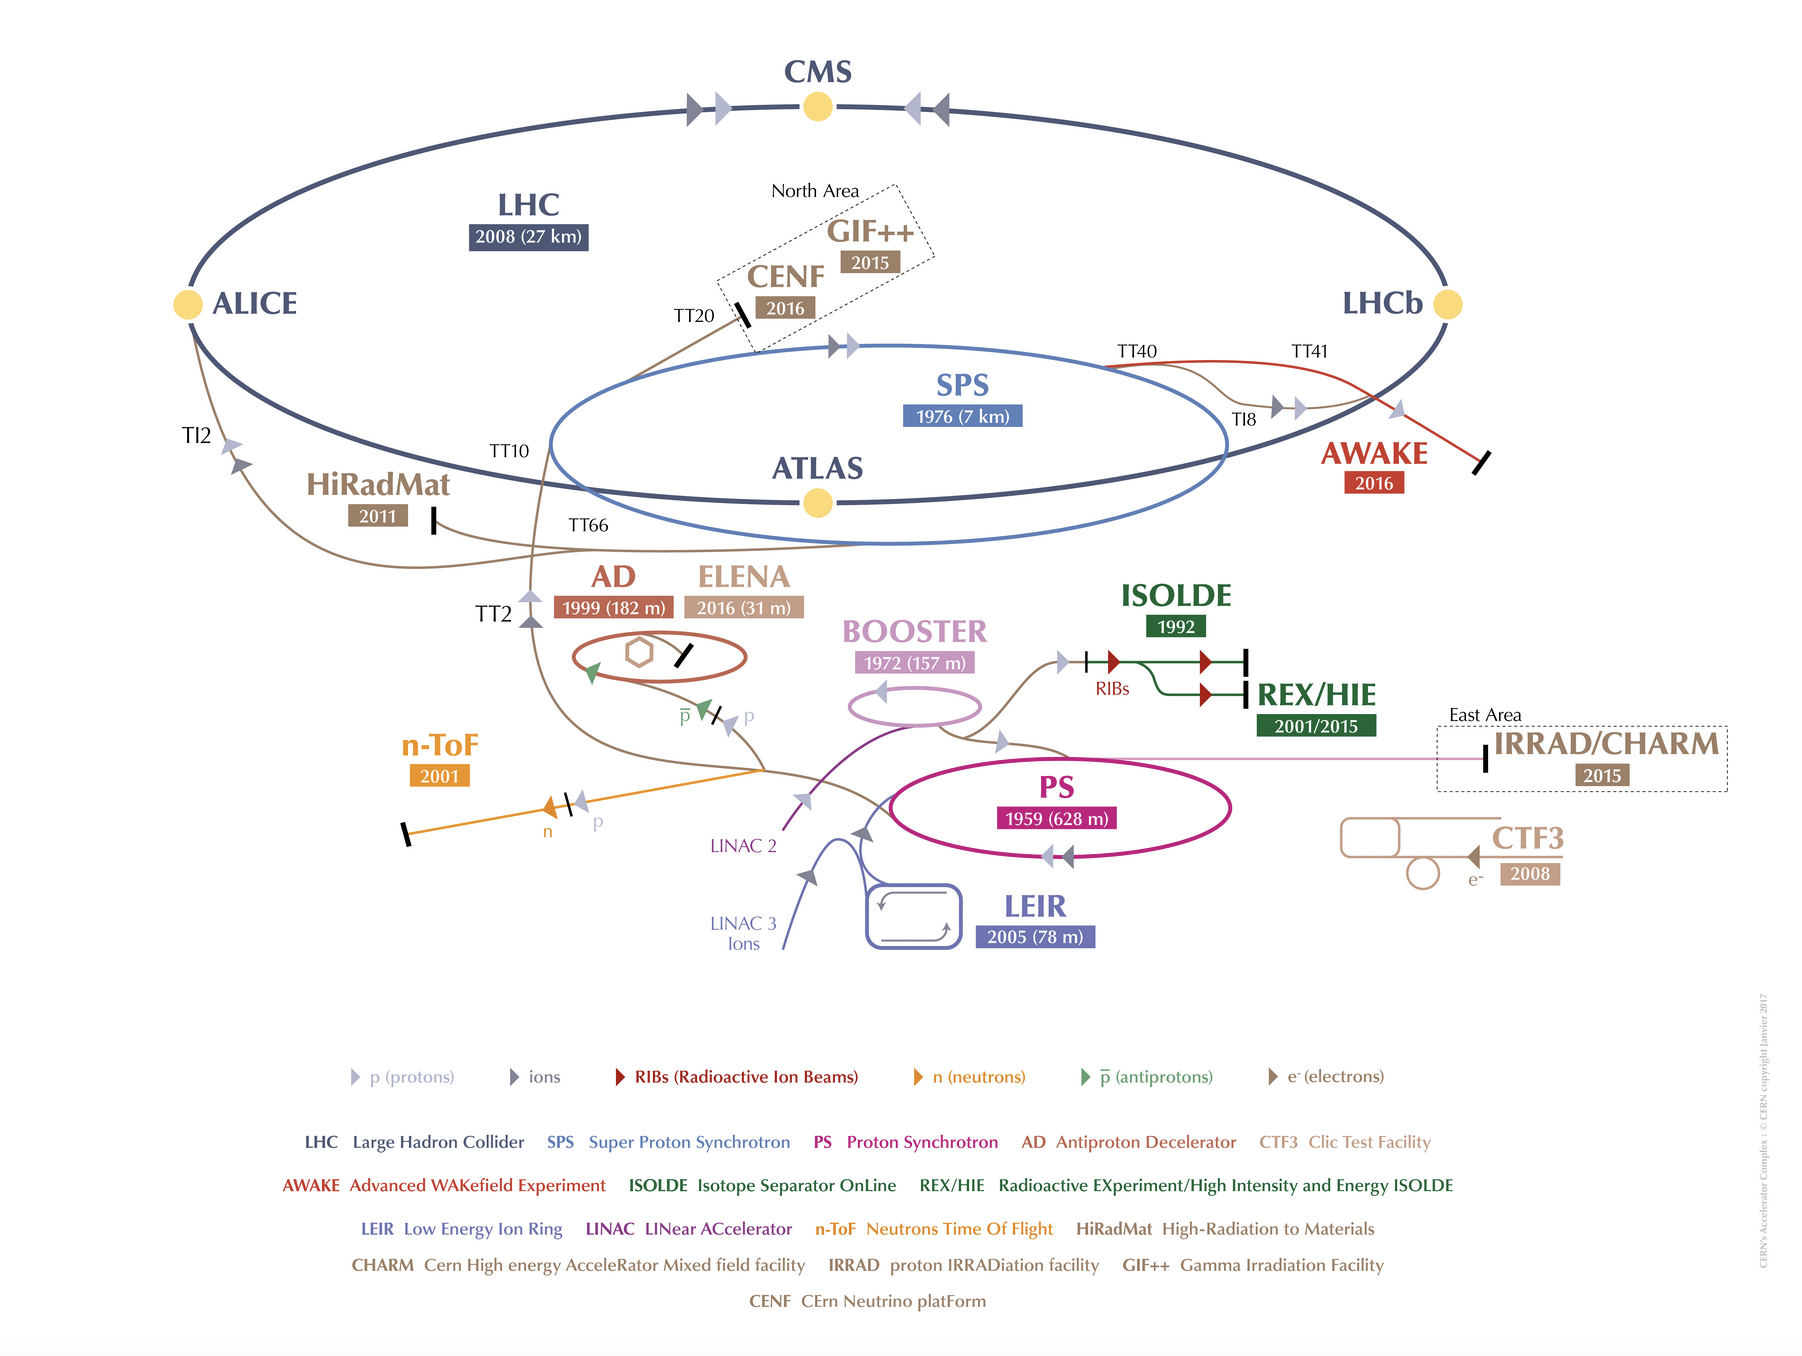
\includegraphics[scale=0.26]{fig/CERNAcceleratorComplex.png}
% 	\caption{The protons used for collisions begin their journey from a bottle of hydrogen \cite{LHCbottle} and they are sent through a series of accelerators to ramp up particle beam energies to 6.5 TeV  }
% 	\label{fig:accelerator_complex}
% \end{figure}

\begin{figure}[!htbp]
	\centering
	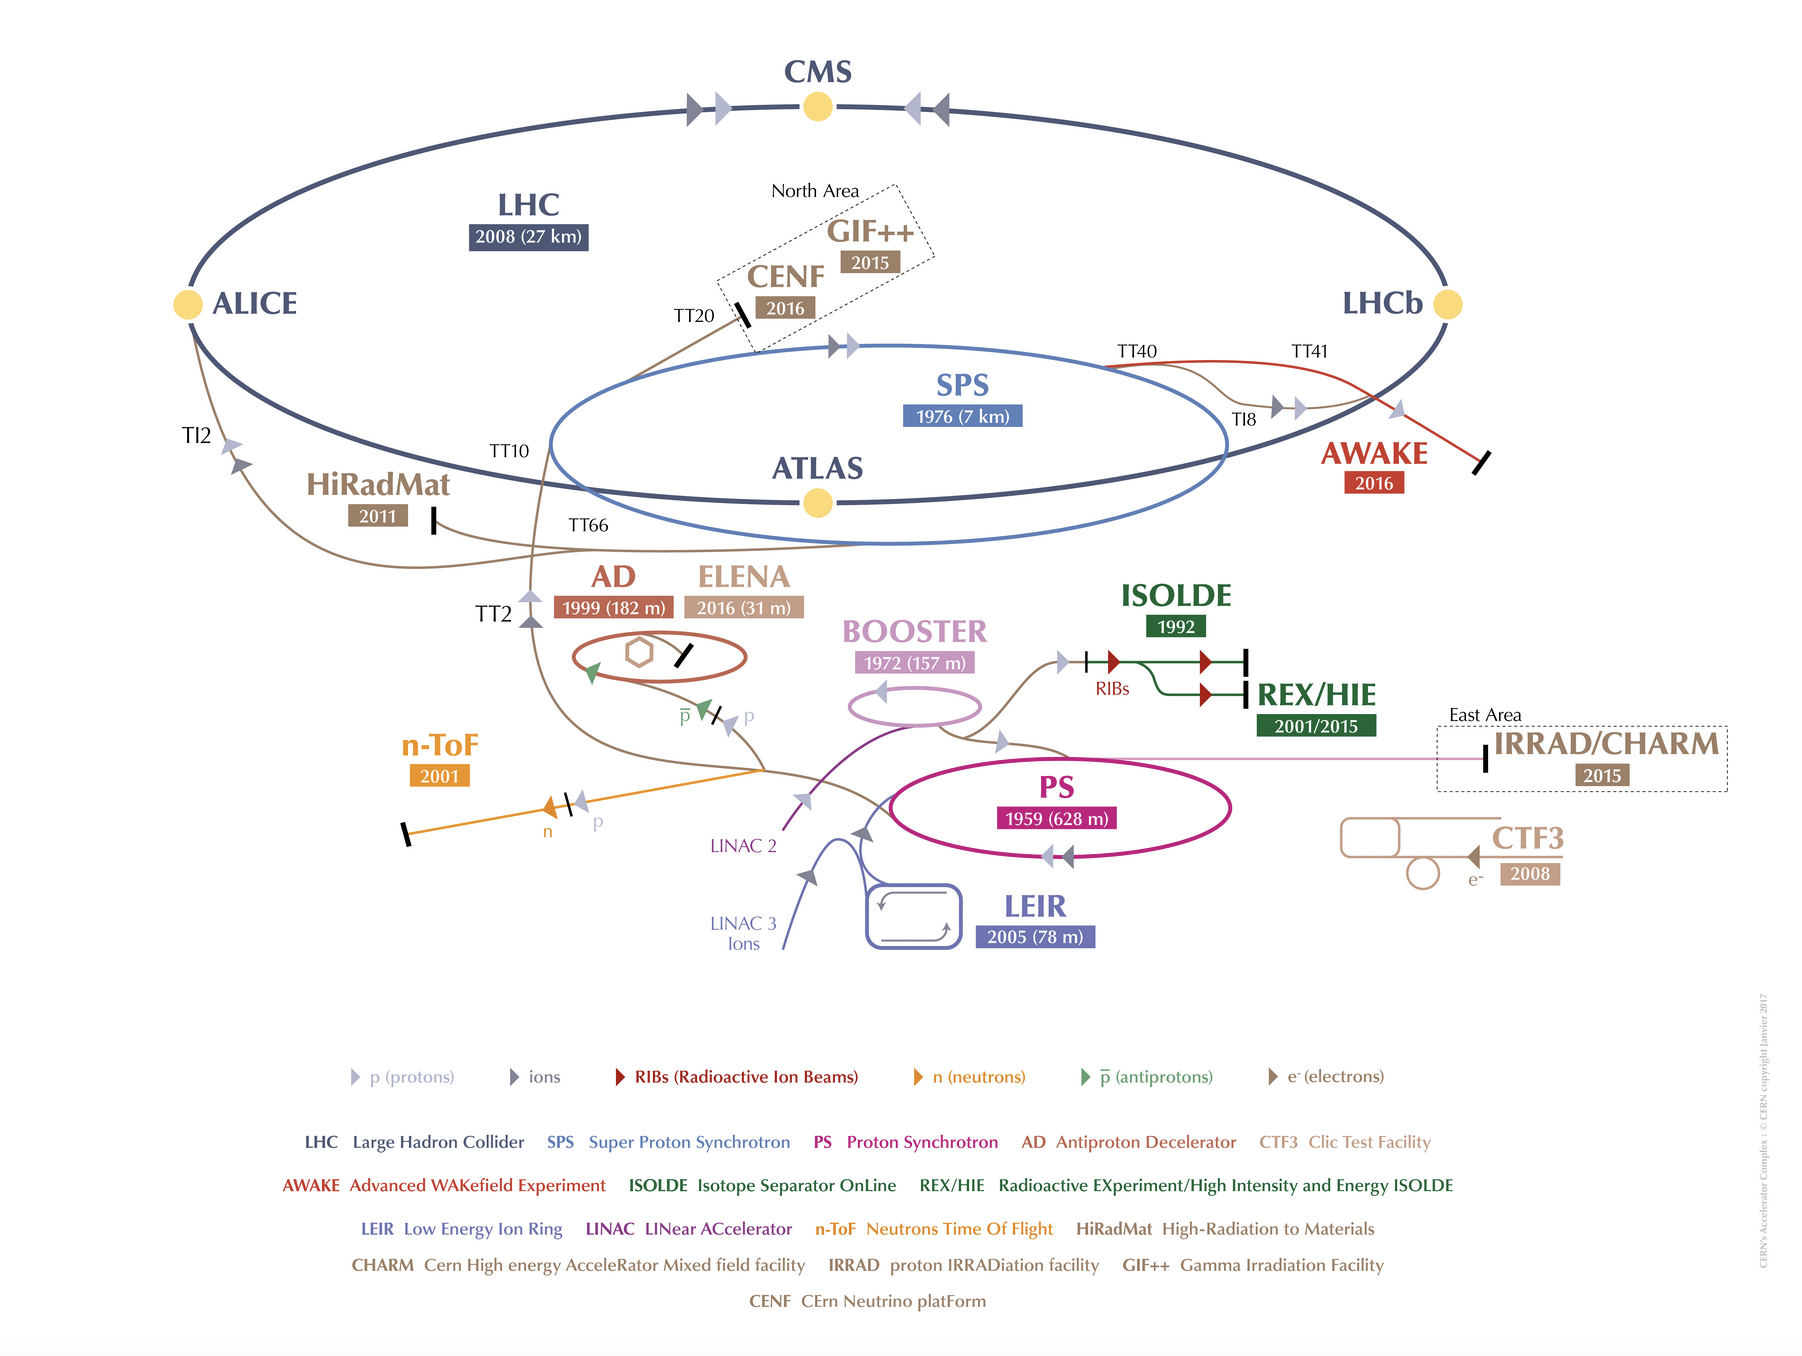
\includegraphics[scale=0.5]{fig/CERNAcceleratorComplex.png}
	\caption{The CERN Accelerator complex has a series of accelerators that ramp up particle beam energies to 6.5 TeV in Run II.}
	\label{fig:accelerator_complex}
\end{figure}

\subsubsection{Collider Design Fundamentals}

Creating new particles and probing the underying structure of matter requires energy and momenta - quantities whose magnitude are dictated by Einstein's equation on Mass-energy equivalence $E^2=(mc^2)^2+(pc)^2$ and de-Broglie's relation. The LHC achieves high energies through its near perfectly circular design with a large radius, $r\approx4$-km. In this section we discuss the advantages and disadvantages of these design choices to guide  future colliders.

Circular colliders have a distinct advantage over linear ones. The first one is high collision rates. Particle beams could circulate over the 27-km ring at a rate of 11 kHz, for many hours allowing it to achieve the highest nominal collision rates at 40 MHz. This collision rate is calculated by multiplying the number of bunches times their revolution frequency - which are experimentally modified. Linear colliders, on the other hand, have the disadvantage of having to be refilled with bunches at each collision. 

% The average crossing rate = number of bunches * revolution frequency = 2808 * 11245 = 31.6 MHz.  Times 19 events per crossing at nominal luminosity gives us our 600 million inelastic events per second." \cite{collisionRatePop}}. 

% To create new particles and to probe the underlying structure of atom, we would need energy. The higher the energy we could produce, the higher the masses of the particles we could probe, the better the resolution \footnote{Energy is related to mass: 
% \begin{equation}
%     E = mc^2 
% \end{equation} 
% where $c$ is the speed of light. For us to probe the underlying structure of matter in better detail, we would also require finer wavelengths or higher momenta as shown with de-Broglie relation given by:
% \begin{equation}
%    \lambda = \frac{h}{p}
% \end{equation} 
% where $h$ is $h = 6.626 * 10^{-34} Js$ and $p$ is the particle momentum.}.

 The drawbacks \cite{Ferrario:2020zwm, Andrews:2022nza} for ciruclar colliders mainly come from synchrotron radiation loss. Circulating charged particles means there are energy losses with the following proportionality rate:
\begin{equation}
    P \propto \frac{q^2}{m^4 R^2}.
\end{equation}
Second, a large magnetic magnetic field is also required to maintain the circular path of the particles. Assuming an idealized homogeneous dipole oriented along the particle orbit, the magnetic field strength required is:
\begin{equation}
    |\vec{B}|= \frac{|\vec{p}|}{qcR}.
\end{equation}

For the LHC, these radiation losses are mitigated by having a large-radius accelerator. This also simultaneously contributes to having a larger magnetic field. Interestingly, the LHC uses the repurposed tunnels of the Large Electron Positron (LEP) Collider, the largest radius of any collider in the world.

The LHC from the name itself, collides hadrons which are composite particles made of two or more quarks. Most hadrons are unstable, in contrast with Protons, or heavy elements like lead (\textbf{Pb}) or gold that have long lifetimes making them good choices for particle collisions. In our analysis, we only examine proton-proton collisions. A complication that arises from colliding a composite particle, is that the full momentum is shared by the actual interacting particles. Electrons, which are point-particles are much simpler, i.e. we know exactly the energy of the initial state, i.e. if we were to collide, an electron and a positron. In their simplest representation, protons (uud), are composed of two up quarks and a down quark and gluons which bind these components together. In addition, sea quarks arise from the energy of gluon splitting. The constituent quarks or gluons, collectively known as partons carry only a fraction of the energy and this fraction is determined by the parton distribution functions. Parton distribution functions give the probability to find partons carrying a fraction x of the proton's total momentum. Apart from the primary collision event or the hard scattering event, there are also softer scattering events which are called underlying events. 

The LHC program transitions to the High-Luminosity (HL-LHC) phase beginning in Run3 and ends by around 2040. At this time, a Future Circular Collider (FCC) is expected to push the energy and intensity frontier of particle colliders, with the aim of reaching collision energies up to 100 TeV \cite{Blondel:2021ema}. Figure~\ref{fig:hl-lhc} shows the LHC and HL-LHC scheduled in different phases, while Figure~\ref{fig:lhcschedule} shows the updated LHC schedule accounting for the delays due to the COVID-19 pandemic.

\begin{figure}[!htb]
	\centering
	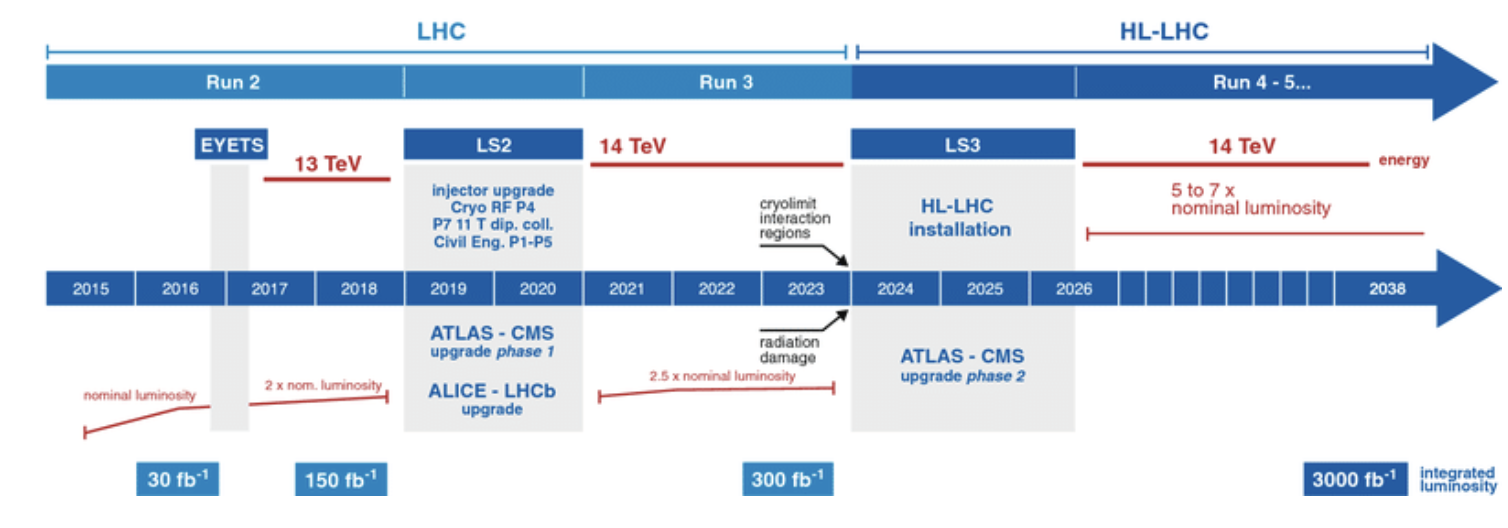
\includegraphics[scale=0.6]{fig/LHC-schedule.png}
	\caption{An overview of the LHC schedule from Run2 onwards before the COVID-19 pandemic delays.}
	\label{fig:hl-lhc}
\end{figure}


\begin{figure}[!htb]
	\centering
	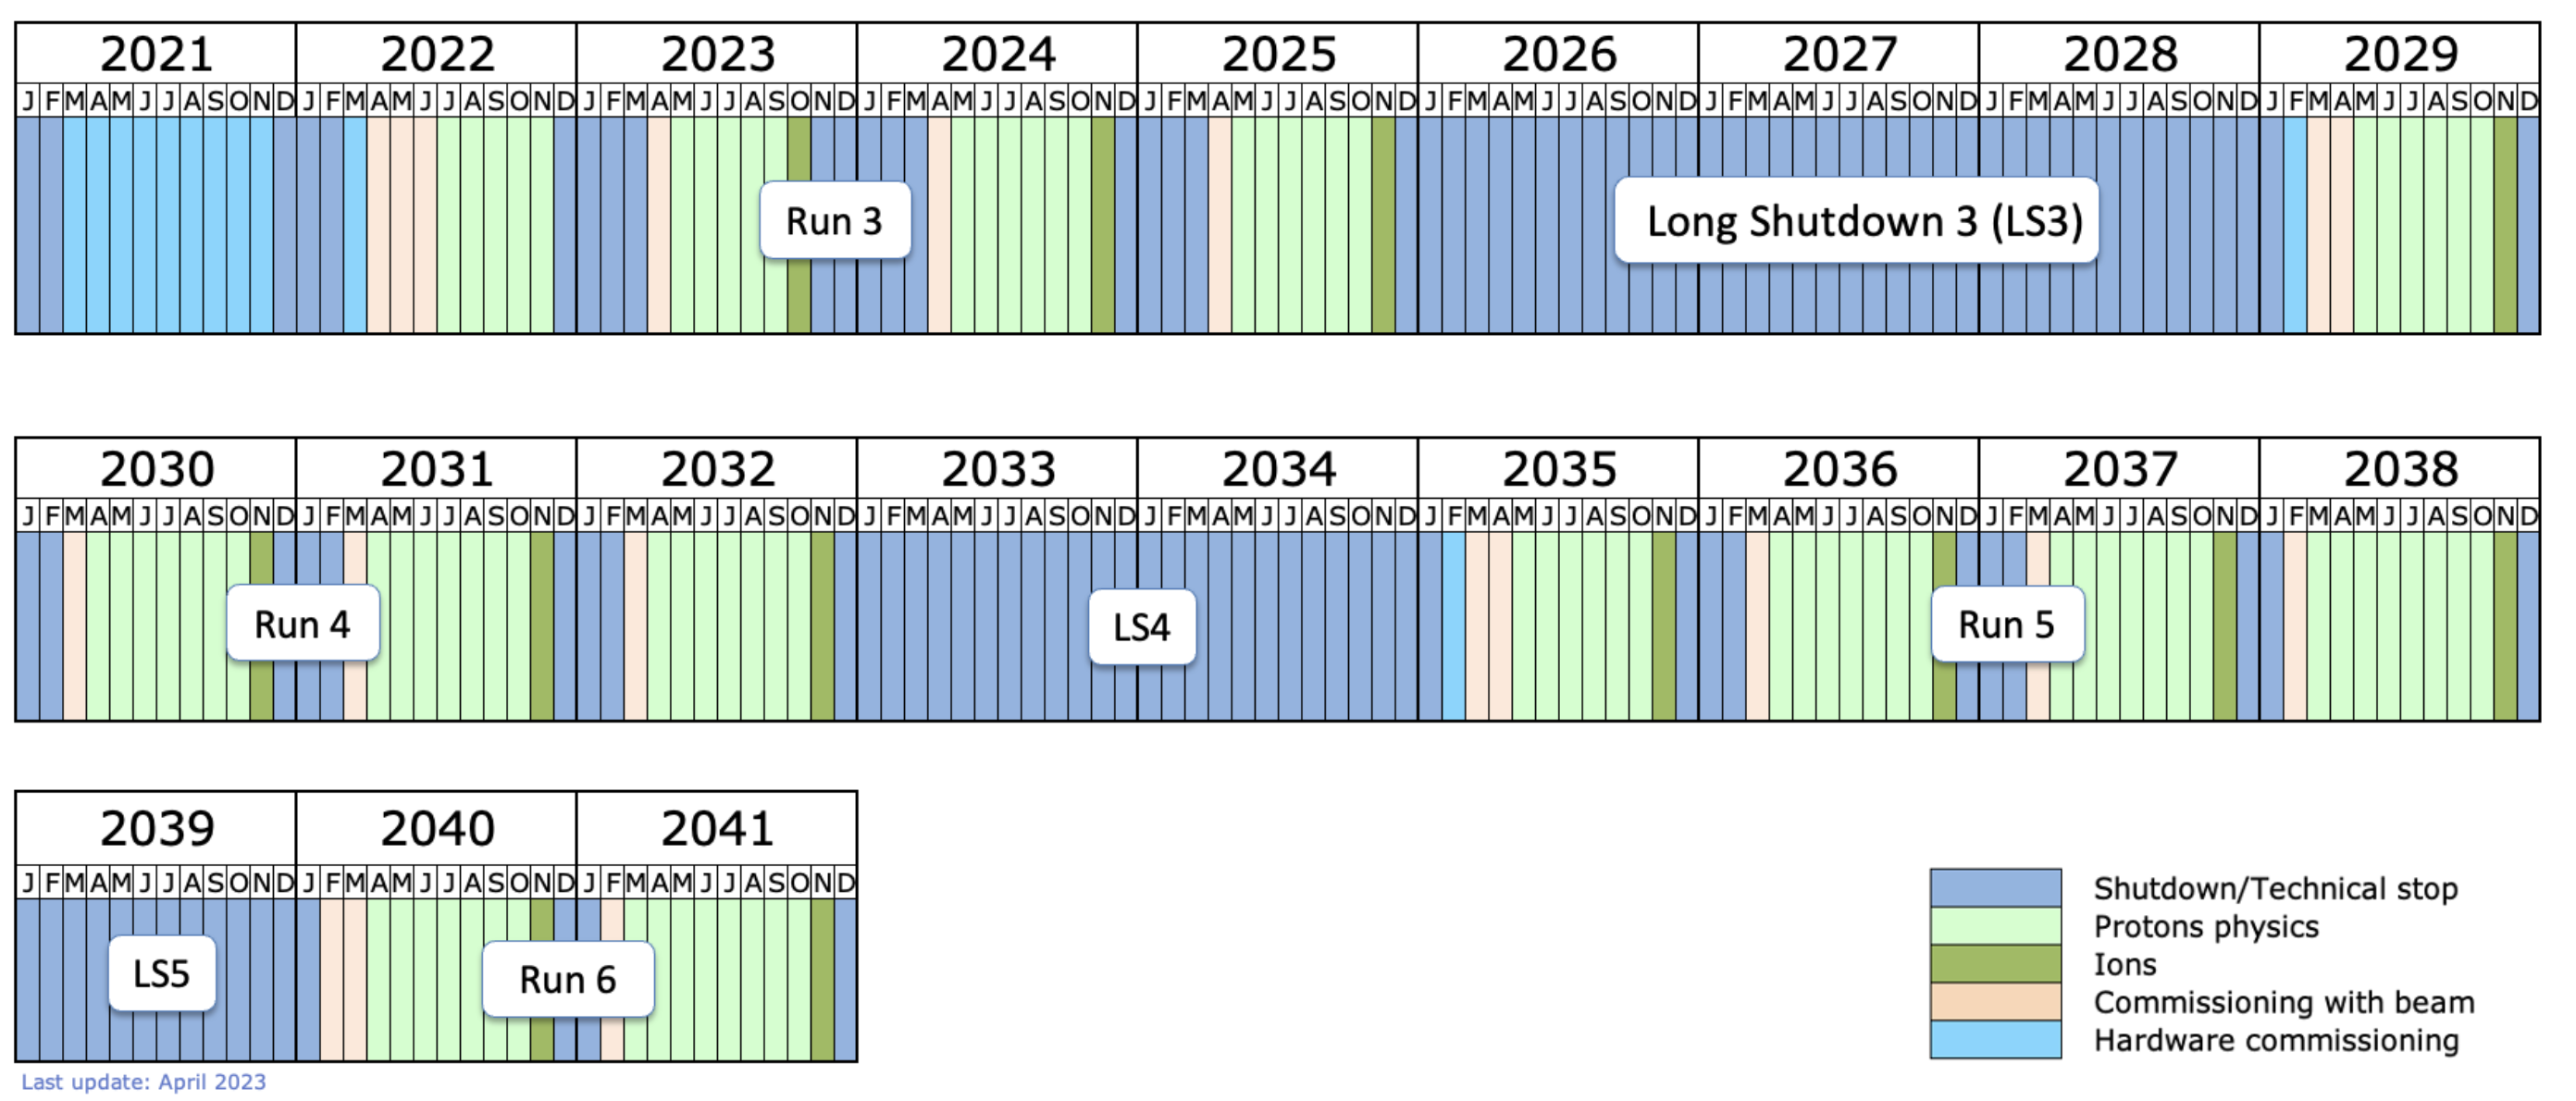
\includegraphics[scale=0.3]{fig/HL-LHC.png}
	\caption{An updated schedule of the LHC accounting for the delays due to the COVID-19 pandemic (Credits: LHC-Commissioning)}
	\label{fig:lhcschedule}
\end{figure}

\section{LHC Schedule, Beam Performance and Pileup}

The LHC operates in production cycles consisting of Runs and Long Shutdowns (LS). In Run 1 of the LHC, which took place from 2010-2012, the LHC operated at 7-8 TeV centre-of-mass energy. This was followed by a 3-year Long Shutdown period where upgrades and repairs were performed. Run 2 started in the summer of 2015 and ended in 2018. During this time, the LHC delivered $163.54$~\fbinv  of data at 13 TeV which surpassed the design luminosity goal of $L = 10^{34}$ cm$^{-2}$s$^{-1}$. This number is generally referred to as the integrated luminosity, $L = \int \mathcal{L} dt$.

The luminosity is different from the collision rate. The proton beam bunches cross at 40 MHz, but not all of the protons within the beam collide as the proton bunches have to be focused into a smaller cross-section.In terms of the beam parameters, the instantaneous luminosity is defined as 

% One could think of luminosity as a beam characteristic. It describes how much of the protons could be squeezed in a beam of a given cross-section. The more particles squeezed in a smaller space, the greater the luminosity. 
\begin{equation} \label{eq:beamParam}
    \mathcal{L} = \frac{N^2_{b}*fn_{b}}{4\pi\sigma^{*}_{x}\sigma^{*}_{y}}F,
\end{equation}

where $N_{b}$ is the beam intensity or the number of protons/bunch; $n_{b}$ is the number of bunches, $f$ is the revolution frequency of the protons, $\sigma^{*}_{x,y}$ are the transverse RMS beam widths at the interaction point; and $F$ is a geometric loss factor that accounts for crossing angle, shape, and longitudinal beam size.

% \footnote{At the LHC this is at 11 kHz with a beam energy of 6.5 TeV}

For a given physics cross-section, the total number of events produced is related to the Luminosity as such:

\begin{equation}
    N_{\textnormal{events} } = L \sigma.
\end{equation}
% To get more events therefore requires a more focused beam which translates to a requirement of higher luminosity.

While higher luminosities provide us more data, it comes with challenges. In each of the proton bunch crossing, multiple simultaneous interactions occur. This problem is known as \textbf{pileup}. This problem can be mitigated by attempts to reconstruct the primary collision vertex but there are also other spurious events that could lead to problems in the reconstruction of physics objects. Additionally, out-of-time pileup can also occur. These arise from collisions coming from prior or later bunch crossings. These factors are major driving forces in the design of CMS algorithms and future detector upgrades. 

% \begin{figure}[tbp!]
% \begin{center}
% 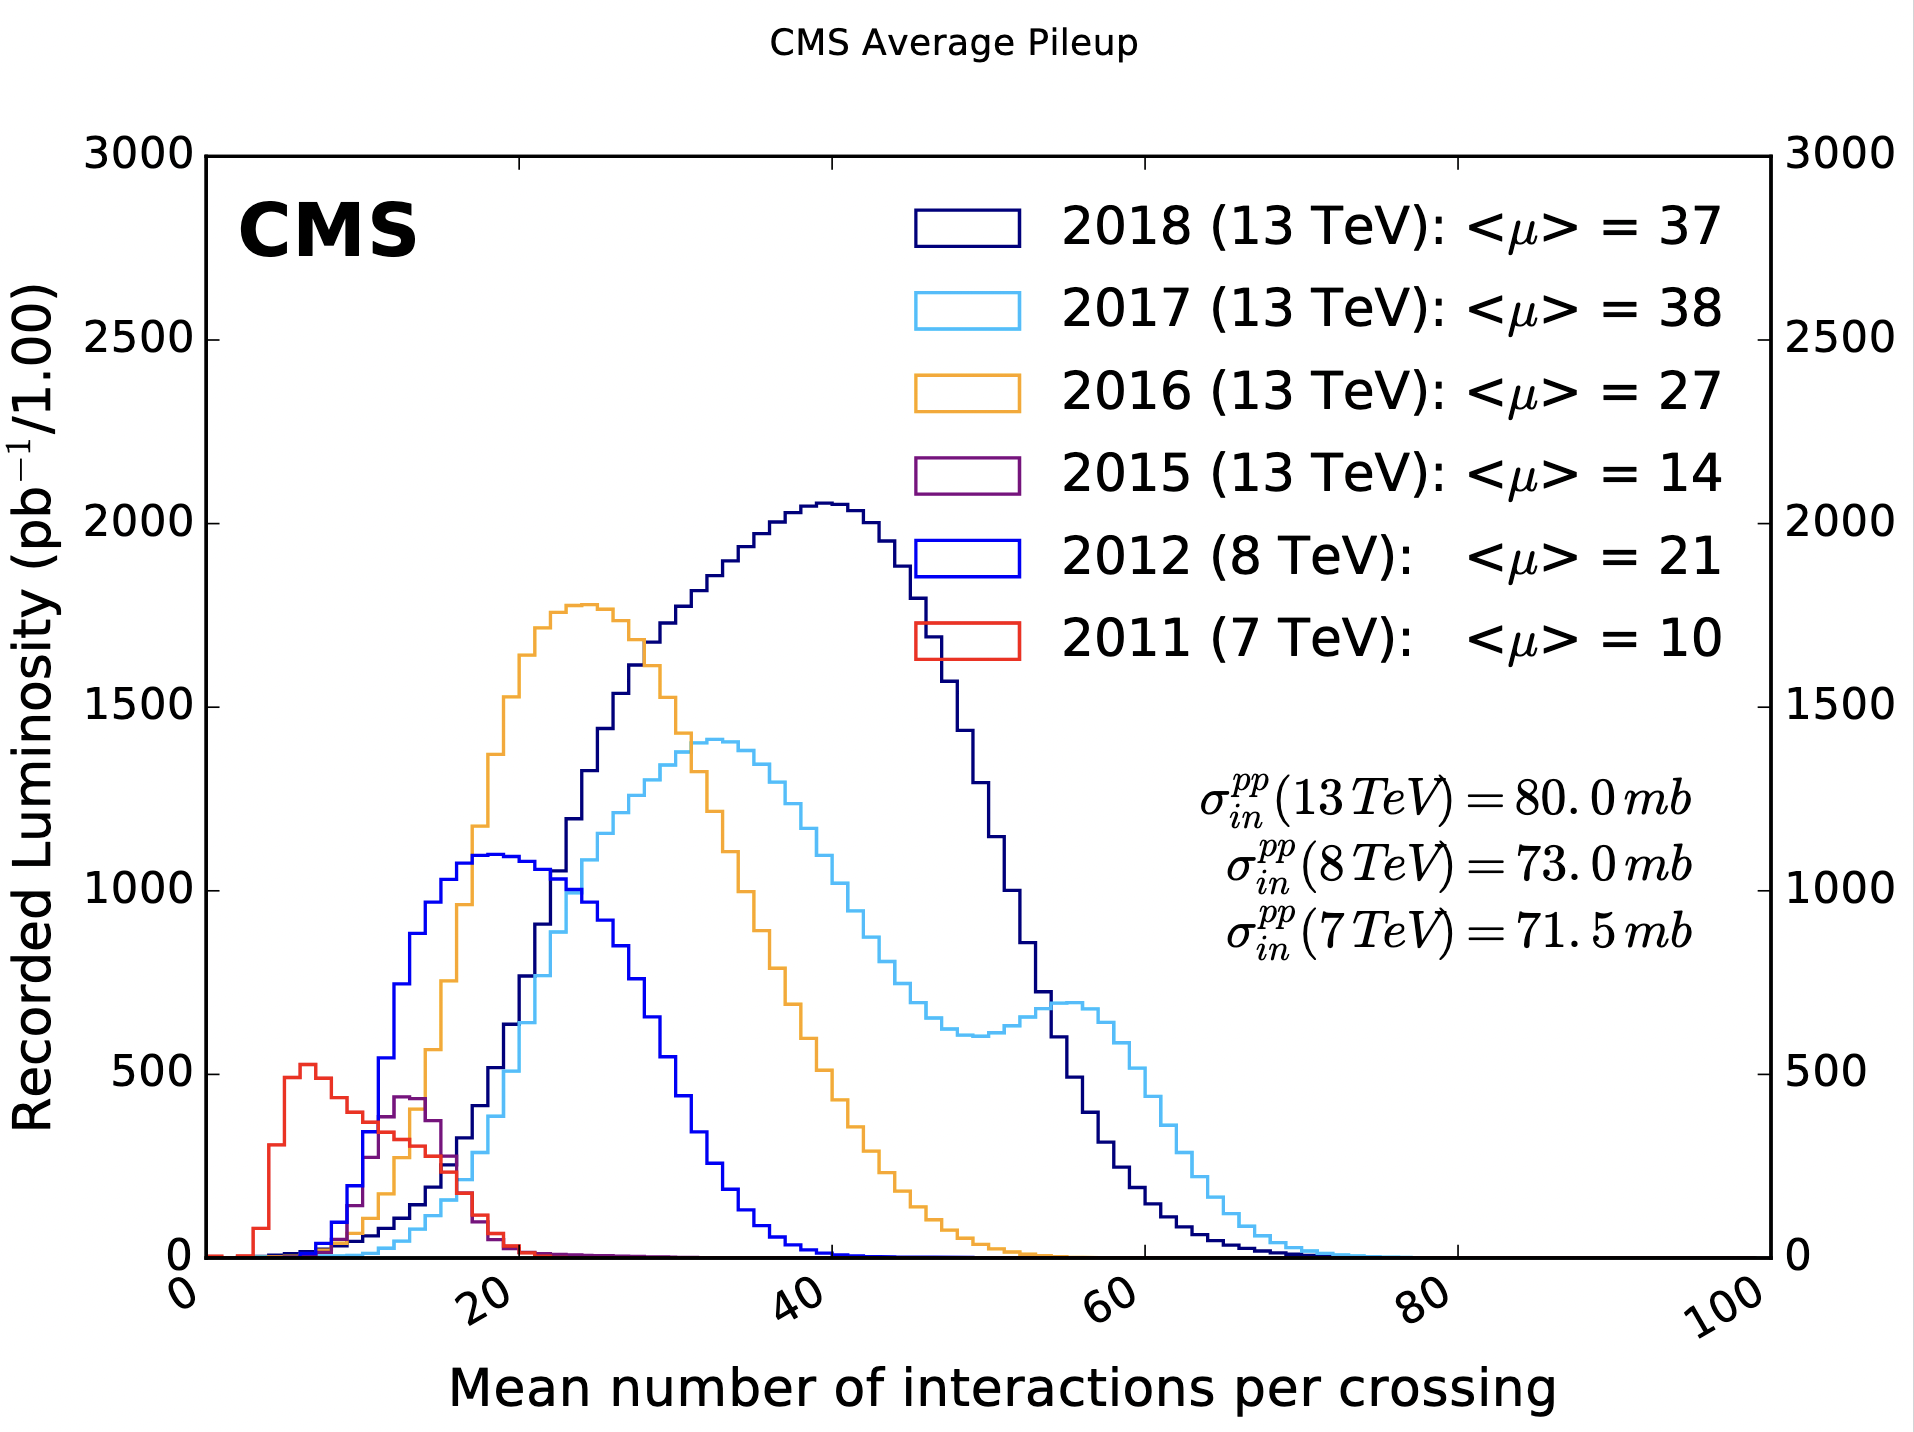
\includegraphics[angle=0,width=0.45\textwidth]{fig/PileUpRun2On.png}
% 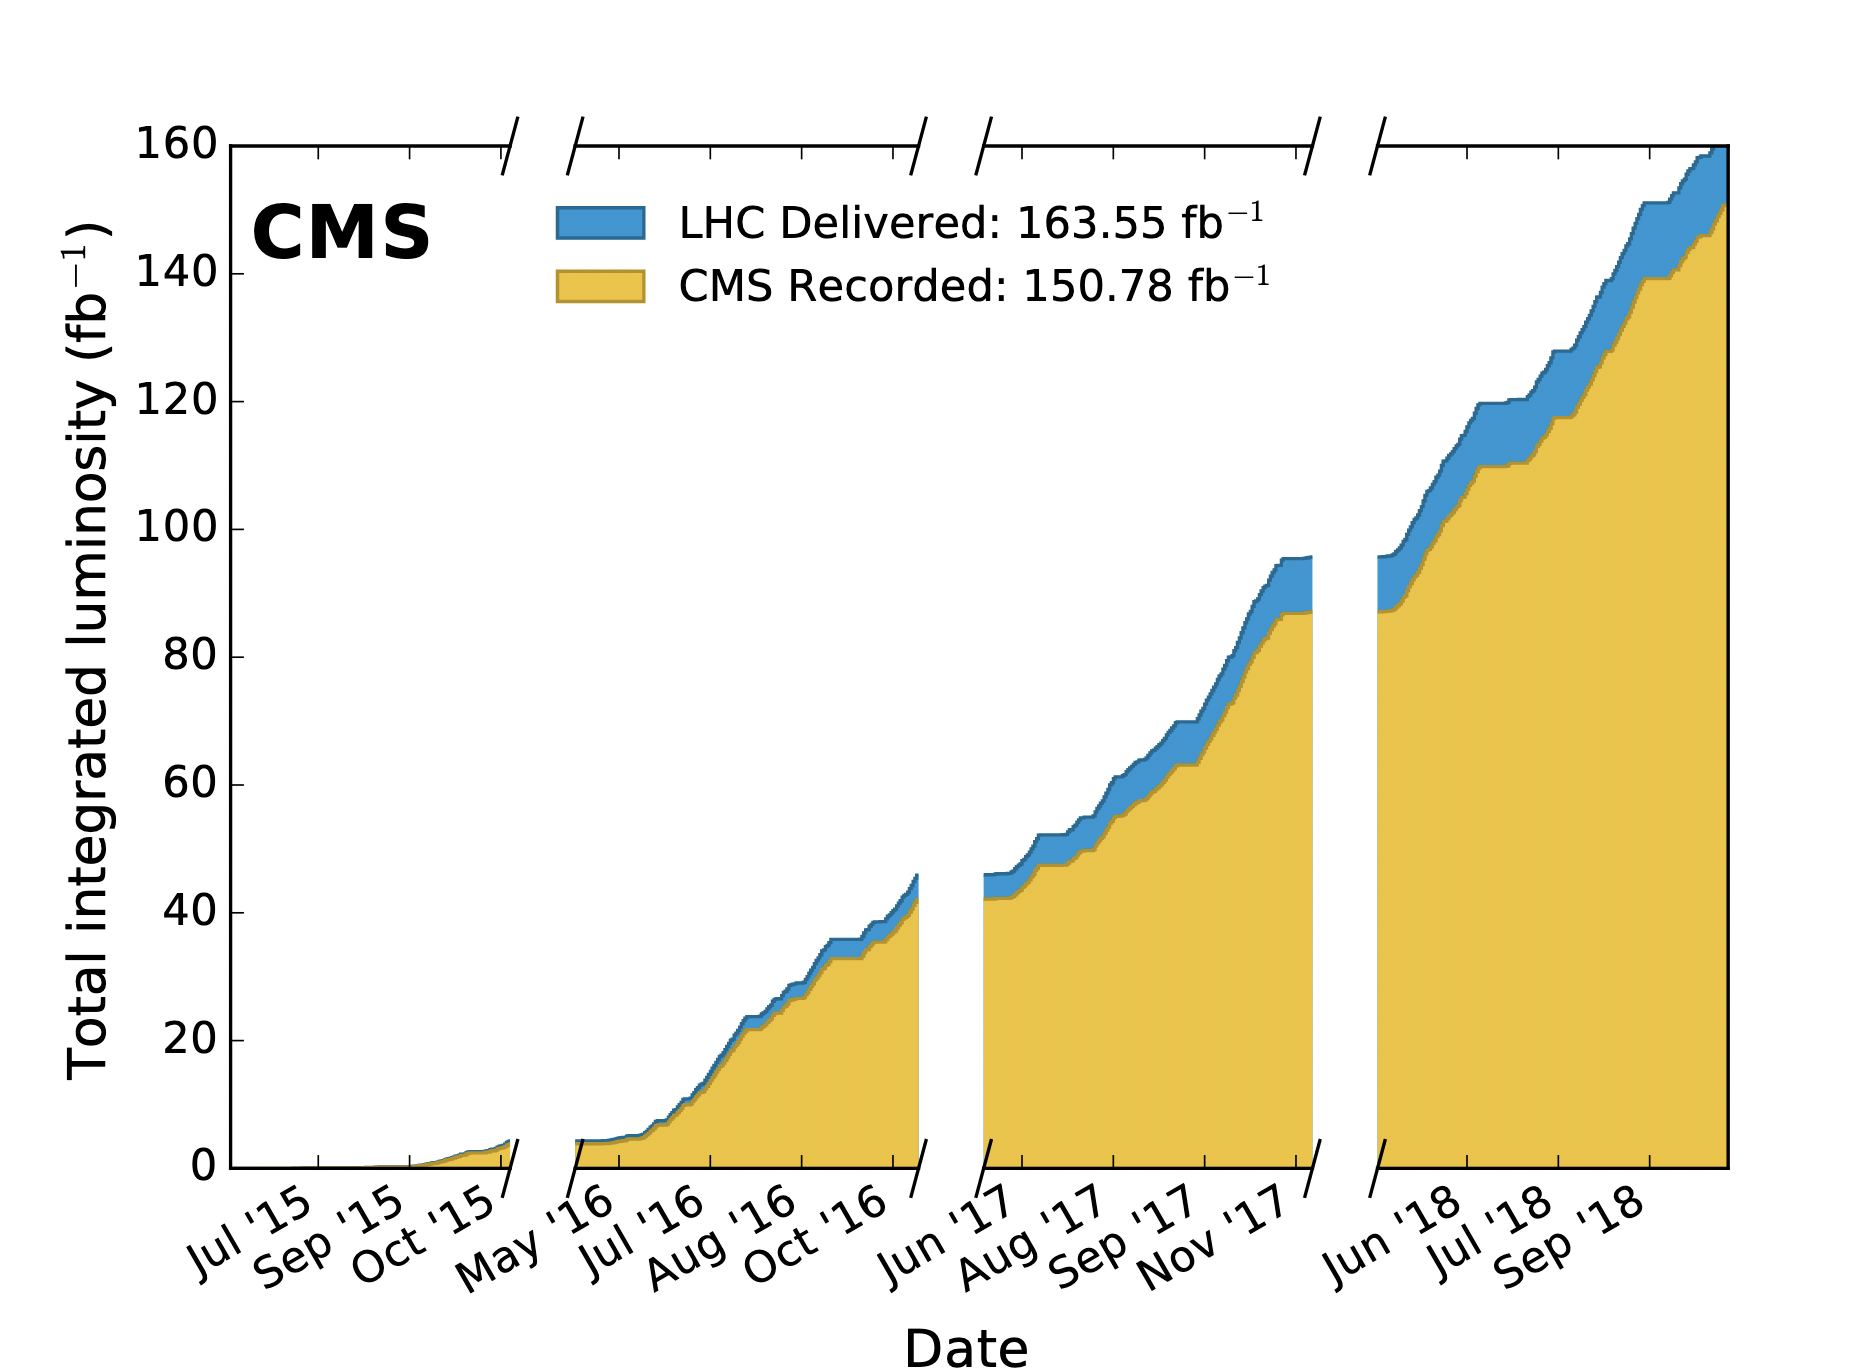
\includegraphics[angle=0,width=0.45\textwidth]{fig/LuminosityRun2.png}
% \end{center}
% \caption{Pileup and Luminosity information from Run II from CMS Lumi Public Results.
% }
% \label{fig:LHCBeam}
% \end{figure}

\begin{figure}[tbp!]
\begin{center}
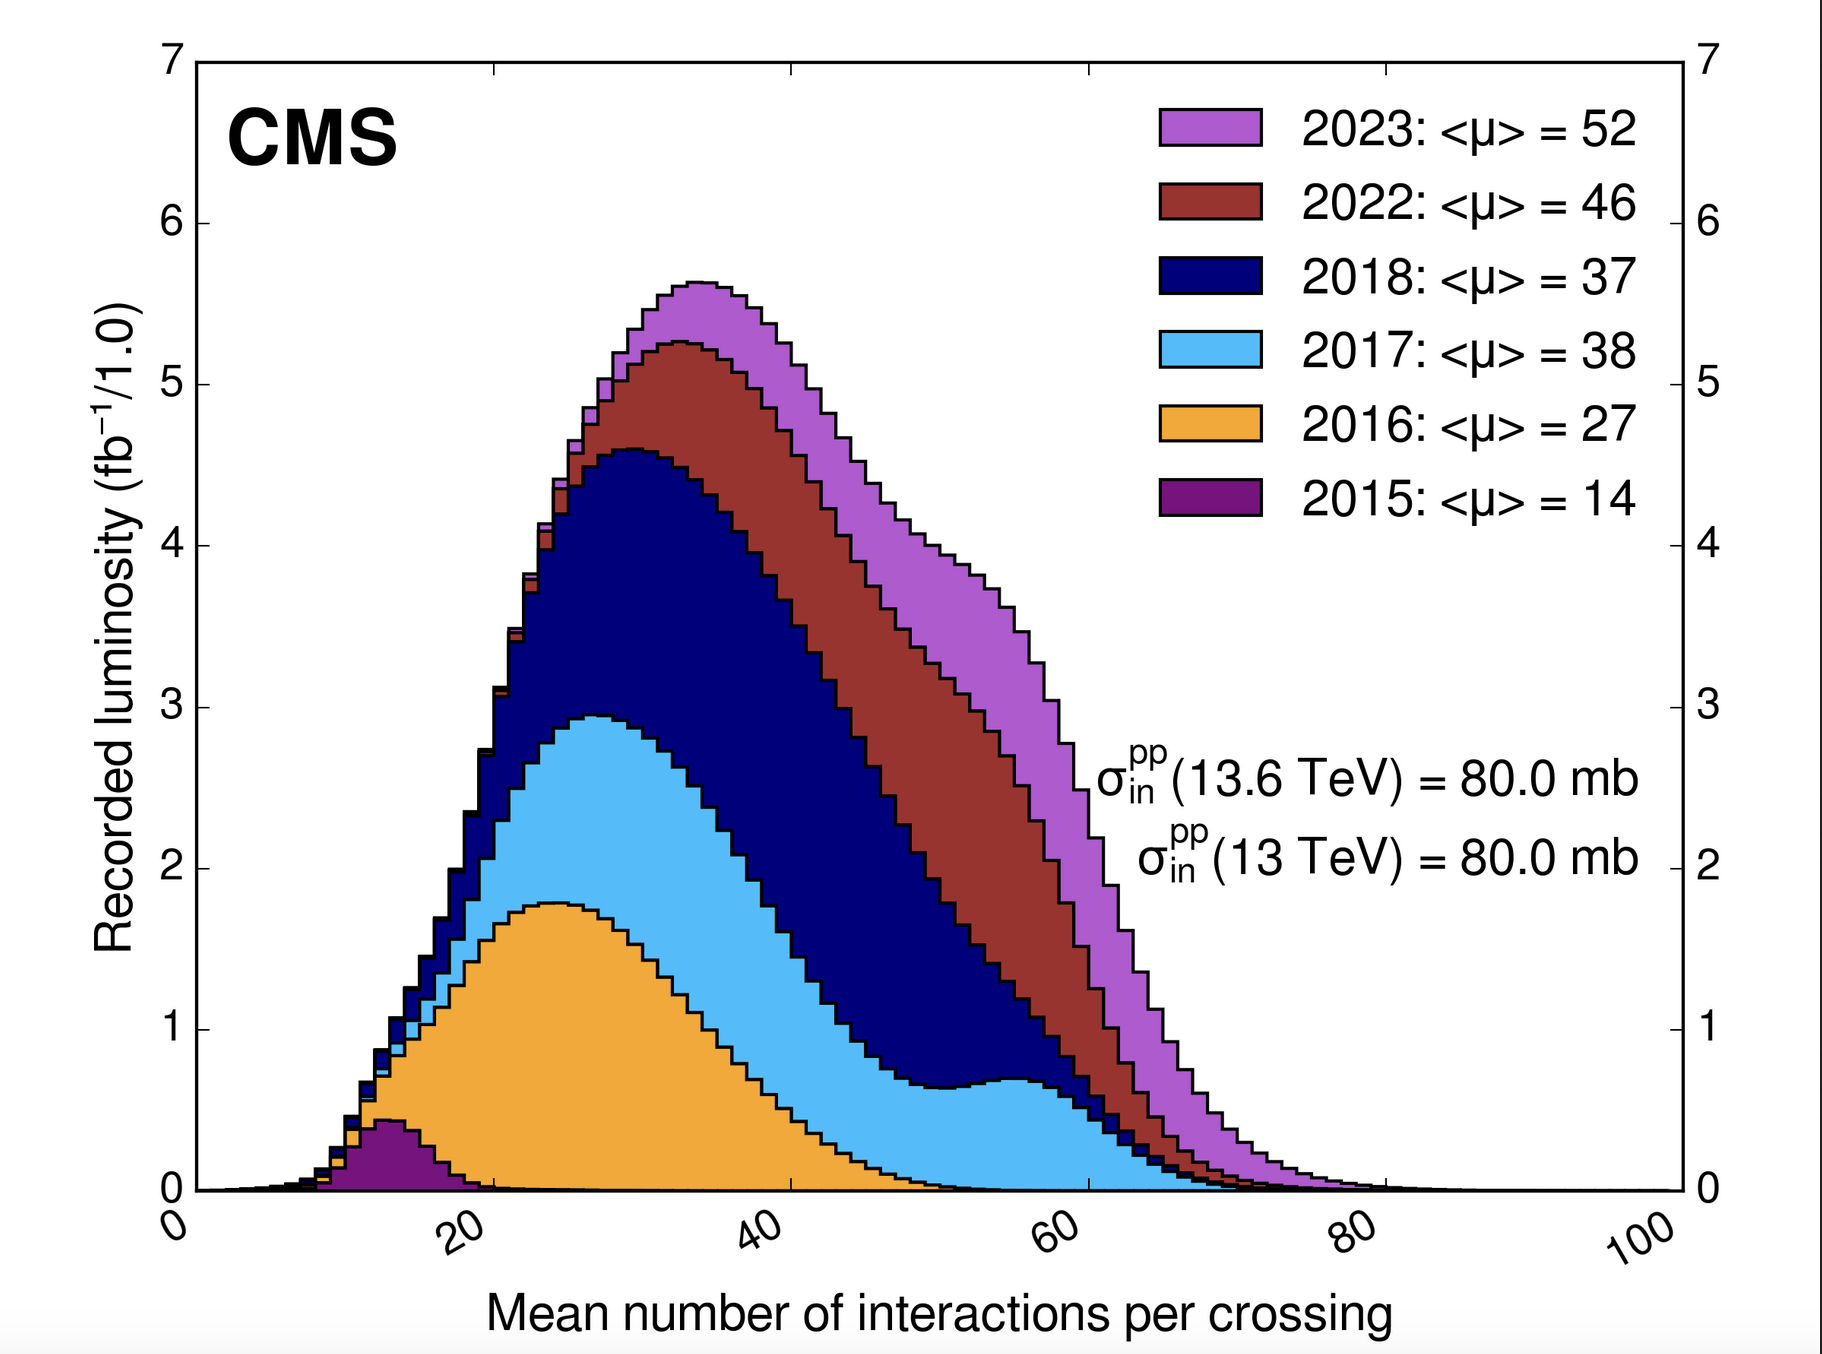
\includegraphics[angle=0,width=0.45\textwidth]{fig/PileupAcrossTheYears.png}
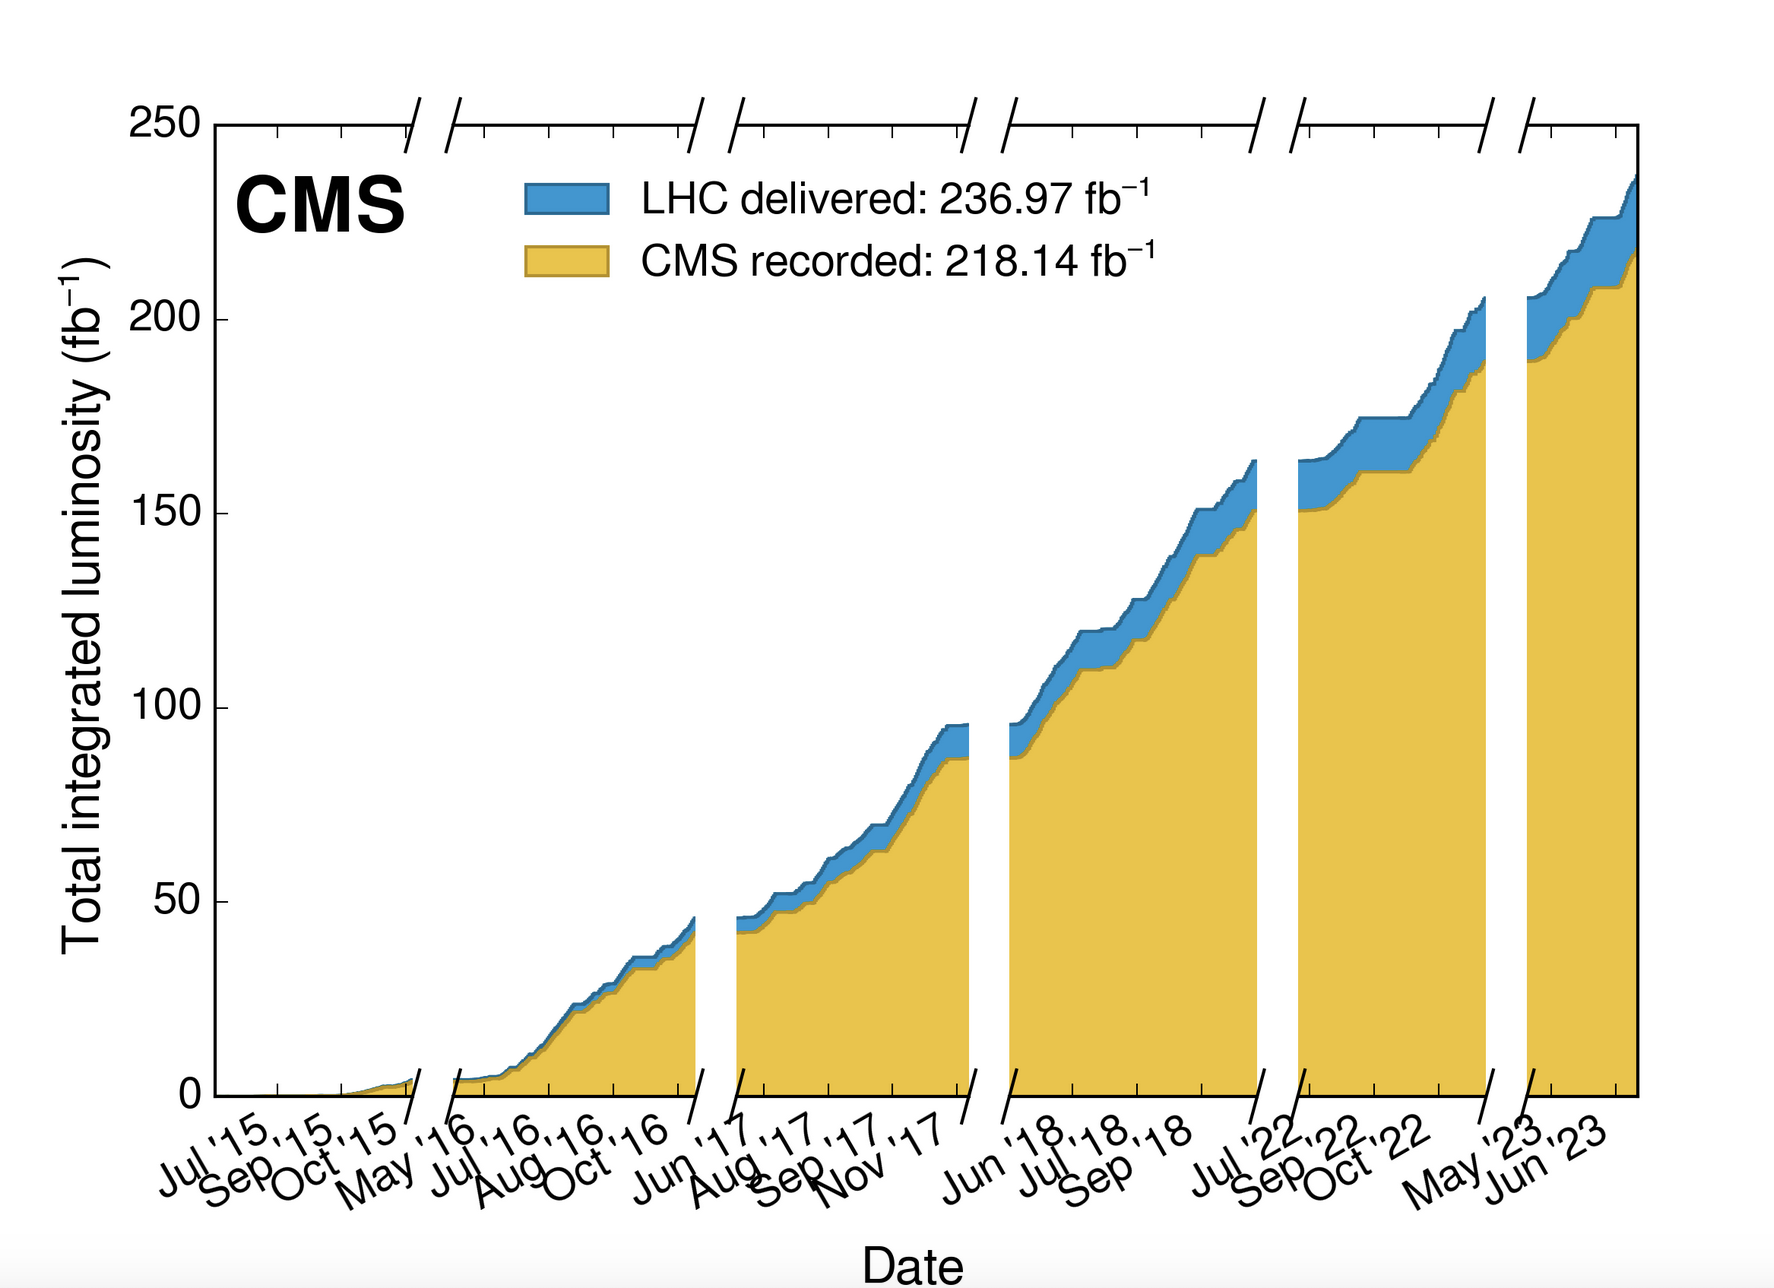
\includegraphics[angle=0,width=0.45\textwidth]{fig/LuminosityAcrossTheYears.png}
\end{center}
\caption{Distribution of the mean number of inelastic interactions per crossing or pileup in data
for pp collisions for various years (left). A total inelastic pp collision
cross section of 69.2 mb is chosen~\cite{CMS:2020ebo}. The Luminosity is shown for various time with white spaces for periods the LHC is not operating (right).}
\label{fig:LHCBeam}
\end{figure}






% idealized homogeneous dipole oriented along the particle orbit, we define the condition for
% a perfect circular orbit as equality between these two forces; this yields the following condition for the
% idealized ring: p
% e = B · ρ, 
%%%
% How many times can proton beams circle around the LHC? 
%
%
%%%

% \feynmandiagram [horizontal=a to b] {
%   i1 -- [fermion] a -- [fermion] i2,
%   a -- [photon] b,
%   f1 -- [fermion] b -- [fermion] f2,
% };

% Linear accelerator\cite{Holzer:2016lud}


%%%%%
% - The Higgs Discovery: https://www.youtube.com/watch?v=so2nCu2Jkbc 
% - How does the LHC work: https://www.youtube.com/watch?v=oWpy0SAAI6E 
% - How does the 
% - https://www.nobelprize.org/prizes/physics/2013/summary/ 
% The Nobel Prize in Physics 2013 was awarded jointly to François Englert and Peter W. Higgs "for the theoretical discovery of a mechanism that contributes to our understanding of the origin of mass of subatomic particles, and which recently was confirmed through the discovery of the predicted fundamental particle, by the ATLAS and CMS experiments at CERN's Large Hadron Collider" 
%%%%%

% - Motivation 
% - the large 
% - proton journey starts from a bottle
% \cite{Evans:2008zzb} \\
% - accelerator complex \cite{Bulletin:1255151} \\ 

% -------------------------------
% - Proton-proton collisions, COM and Luminosity \cite{Bulletin:1255151} \\
% - ALICE \cite{ALICE:2008ngc} \\
% - CMS  \\
% - ATLAS \cite{ATLAS:2008xda}\\
% - LHCb \cite{LHCb:2008vvz} 
% - LHC schedule, CMS mass energies, pileup mitigation \cite{CMS:2020ebo}
% \section{CMS Experiment - Detector}
% The CMS detector\cite{CMS:2008xjf} \\ 

% Copy paste chunks from here:
% https://twiki.cern.ch/twiki/bin/viewauth/CMS/Internal/PubDetector

% Maybe add something from the TDR  \cite{CMS:2008xjf}
% ----------------------------------
% \subsection{Detector Coordinates}
% Nice discussion by Afiq \cite{Anuar:2019rft}
% \subsection{Particle Interaction with Matter}
% Mike has a very nice discussion here\cite{Andrews:2022nza}
% \subsection{Subdetectors}

% \subsection{CMS ECAL}

% % \subsection{Magnet}
% % \subsection{Inner Tracking System}
% precision tracking \cite{CMS:2018wqs}
% \subsubsection{Electromagnetic Calorimeter}
% Photons, calorimeter, lead-tungstate module 
% General description of passage of particles in materials \cite{ParticleDataGroup:2018ovx} \\
% \subsubsection{Hadron Calorimeter}

% Upgrade \cite{Cooper:2016kef}
% % \subsection{Muon System}
% Design and performance of the wedges\cite{CMSHCAL:2007zcq}

\section{CMS Experiment and Its Subdetectors}~\label{sec:CMSDetector}
The CMS detector (Figure~\ref{fig:CMSdetectorCutaway}), is one of general-purpose detectors of the LHC which collects the data generated at the CMS interaction point found in P5 in Cessy, France. The detector has a series of concentric cylindrical layers which comprise the Barrel region of the detector. To capture collision products going in the more forward regions, at angles moving closer to the beam line, Endcap detectors are also constructed. These layers hermetically seal the central collision point.

The CMS uses a coordinate system that is centered at nominal interaction point which is found halfway through the cylinder axis of the detector. The z-axis goes through the beam pipe, and the radial coordinate, r is measured from this axis. The angular coordinates $\phi$ and $\eta$ are defined as follows, $\phi$ corresponds to the azimuthal angle or the horizontal angle going clockwise around the z-axis, and $\eta$ is the pseudorapidity which is related to the angle $\theta$ by the equation (see Figure~\ref{fig:etatheta}),

\begin{equation}
    \eta = -ln (tan(\theta/2)).
\end{equation}

\begin{figure}[tbp!]
\begin{center}
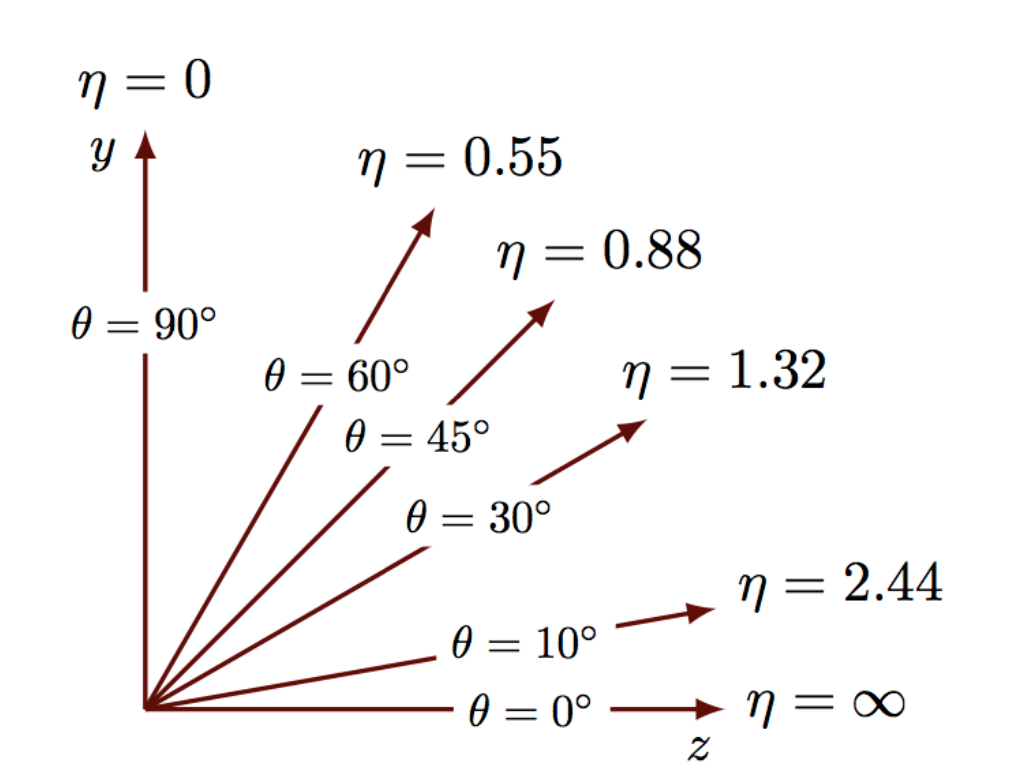
\includegraphics[angle=0,width=0.50\textwidth]{fig/pseudorapidity.png}
\end{center}
\caption{The relationship between $\eta$ and $\theta$.
}
\label{fig:etatheta}
\end{figure}


From the interaction point, collision products traverse layers of materials that are designed to identify, and absorb the energy of most of the particles. These layers are assembled in the following order: 1.) Tracker System, 2.) Electromagnetic Calorimeter, 3.) Hadron Calorimeter, 4.) Muon System. The particles first traverse the Silicon Tracker system which records the position or ``hits" of charged particles. 


The CMS silicon tracker system, records particle paths accurately but are of lightweight material such that they disturb the particle trajectory as little as possible~\cite{CMS:2008xjf}. In addition, they tolerate high radiation fluxes since they are close to the interaction point. Combining the information collected one could reconstruct charged particle $p_T$, and the particles could be traced back to a specific vertex. This information is used in pileup mitigation. 

The next two layers of the CMS detector are the calorimeters that measure the energies of electromagnetic and hadronic particles. Particles going through matter produce a shower, where each interaction with atomic nuclei produces secondary particles, which goes into a repetitive process of cascading particles until the full energy of the initial particle is spent. Ideally, full shower should be captured by the calorimeter so that a more accurate energy value could be reconstructed. We discuss them in more detail in the next two subsections.

Finally, the Muon system characterizes the muons which are minimally ionizing and can escape the calorimeters due to their long life-times and low-energy deposition characteristics. The muons identify muons, measure their momenta, and provide signals for triggering on them via four complementary systems arranged in the steel flux-return yoke of the CMS solenoid. These systems cover a large range of pseudorapidity. The location of the magnetized steel behind the calorimeters and solenoid ensures a low probability of penetration by non-muon or non-neutrino candidates. 

The drift tube system (DT) in the barrel covering $|\eta| < 1.2$ has the task of providing precise spatial measurements and trigger information through drift chambers with rectangular cells. Next, a cathode strip chamber (CSC) system in the endcap covers the forward region with pseudorapidity $0.9 < |\eta| < 2.4$. It has the same task as the DT but is comprised of a different material because of the higher flux of particles in the endcaps, and it also has a faster response time. Additionally, RPCs or resistive plate chambers -- double-gap chambers operated in avalanche mode are placed in both the barrel and endcap to complement the DTs and RPCs to unambiguously identify the bunch crossing corresponding to a muon trigger candidate. It also has a rapid response time~\cite{CMS:2023gfb}.

\begin{figure}[tbp!]
\begin{center}
% 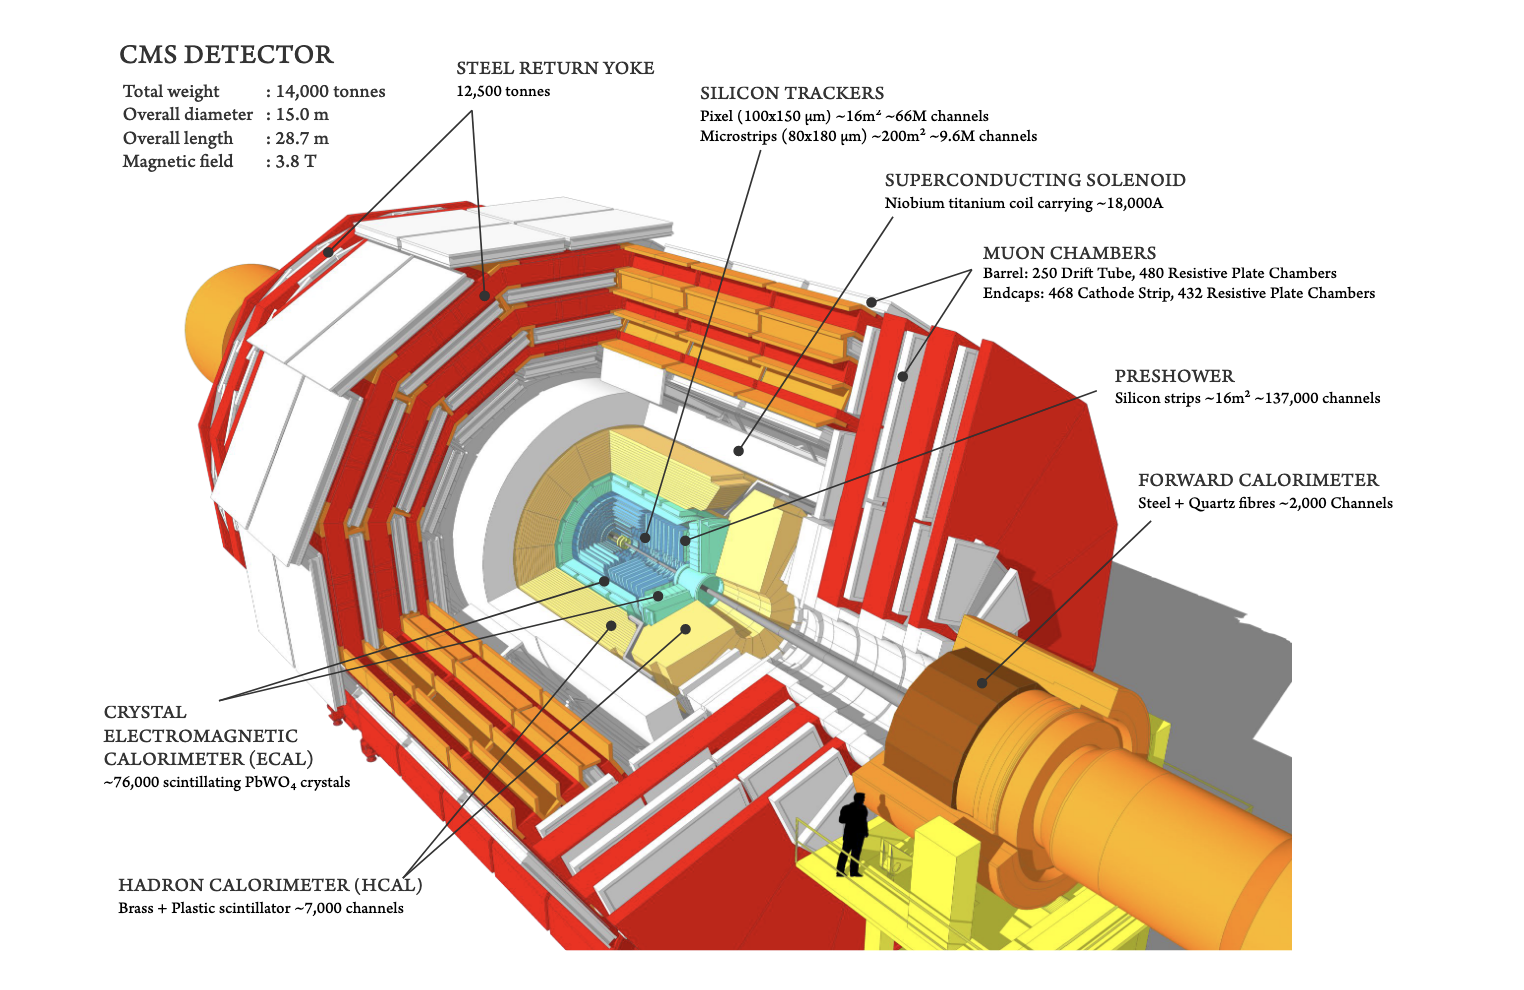
\includegraphics[angle=0,width=0.50\textwidth]{fig/CutawayViewCMSDetector.png}
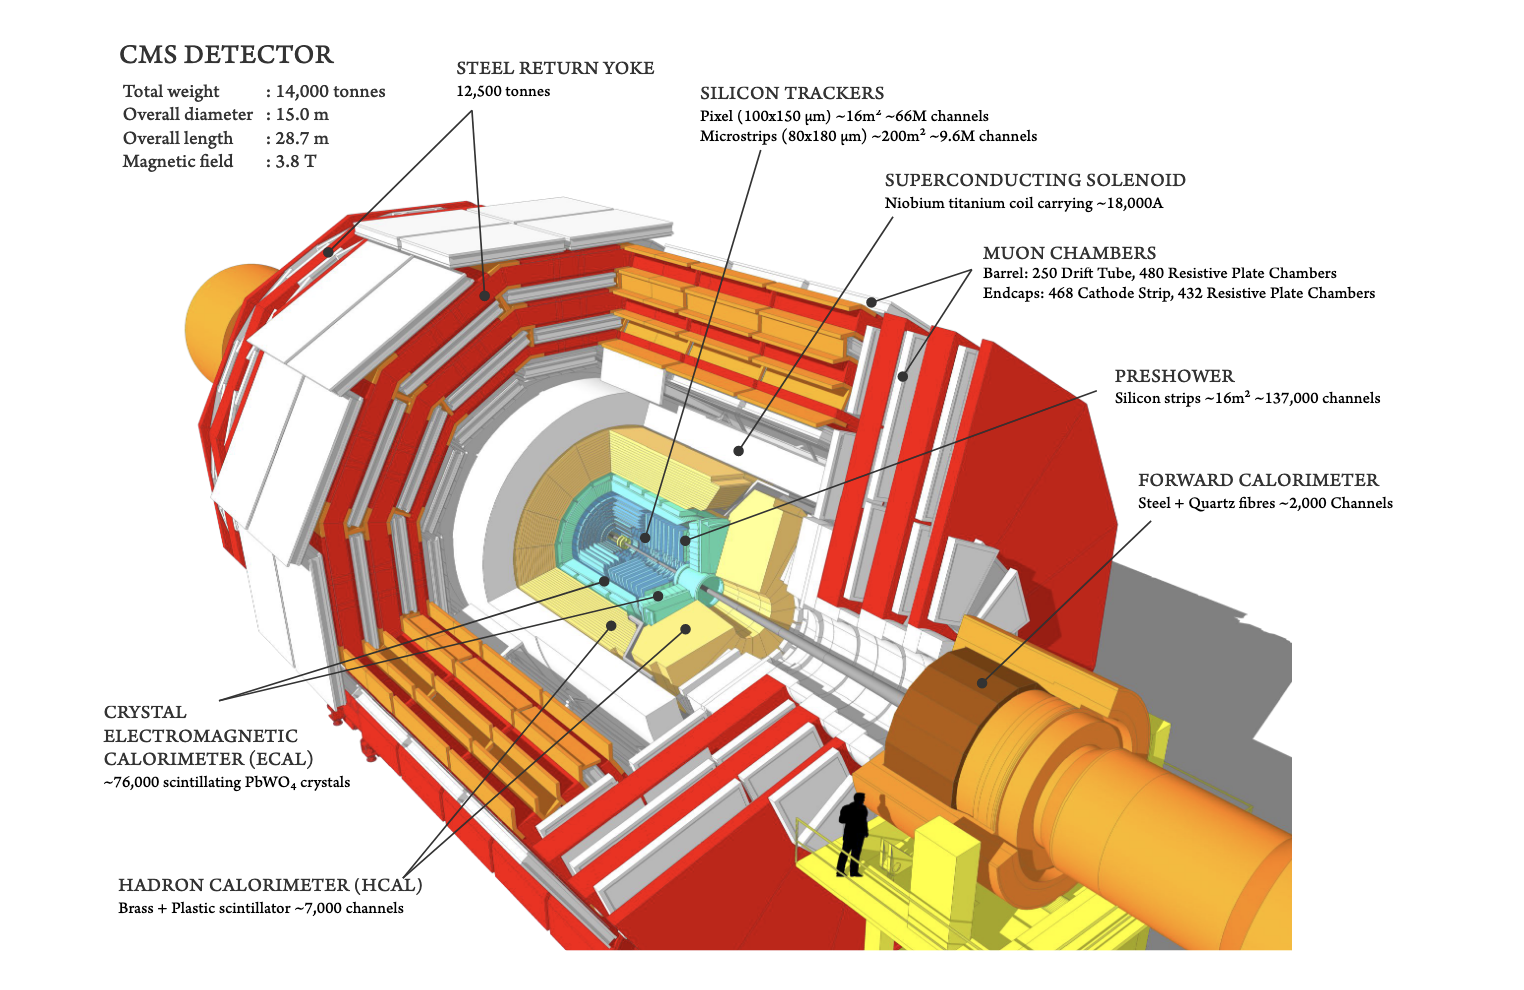
\includegraphics[scale=0.5]{fig/CutawayViewCMSDetector.png}
\end{center}
\caption{A cutaway view of the CMS detector showing its components~\cite{Sakuma:2013jqa}.
}
\label{fig:CMSdetectorCutaway}
\end{figure}

\subsection{ECAL}

The Electromagnetic calorimeter or ECAL, is the second layer of subdetectors that particles go through after the tracker. The ECAL is designed to measure the energies of particles that interact electromagnetically, particularly photons and electrons. It is made of a homogeneous and hermetic lead tungstate (PbW$\text{O}_4$) crystal calorimeter. Homogeneous calorimeters act both as absorbers and scintillators.
As the incident particle interacts with the atomic nuclei of the crystal, electromagnetic showers are induced. Ionization is induced in the atoms and light is emitted as they de-excite. In short, the scintillators convert energy from the showers to light that is in proportion to the incident particle's energy.

There are about 75000 lead tungstate crystals, 61200 of those are spread across the barrel section (EB), located 1.29 meters from the beam line, and the rest are placed at the circular endcaps (EE) which are at $\pm 3.14$ m from the detector origin. Each endcap seals the barrel, with 7324 crystals which gives coverage up to $|\eta| < 3.0$. The EB covers a pseudorapidity range of $|\eta| < 1.479$ where the crystals are laid out in a $170\times360$ $\eta$-$\phi$ grid. In the EE, the crystals are placed in an x-y grid, with a pseudorapidity coverage of $1.479 <|\eta| < 2.5$. 

There are dimensional differences in the EB and EE crystals. The EB crystals have dimensions of about $22\times22$ mm$^2$ in the front-and-rear-facing sides and are 230 mm is in length, corresponding to 25.8 radiation lengths $X_{0}$. The radiation length of a material is the mean length for an electron to lose all but $1/e$ of its original energy. The EB gives a $\Delta \eta$-$\Delta \phi = 0.174\times0.0174$ granularity. To prevent particles from slipping through the spaces in between, the crystals are tilted at 3$^{\circ}$ with respect to the interaction point normal. The endcap crystals have dimensions of $28.6\times28.6$ mm$^2$ in x-y and has a length of 220 mm which corresponds to 24.7$X_0$. 

To facilitate assembly of the detector, the crystals are arranged into groups supermodules in the EB and supercrystals in the EE. There are 36 identical supermodules in the EB and each of these covering half of the barrel length. The supermodules are made up of 4 modules that containe 2 rows of 5 crystals. In the EE, the supercrystals are $5\times5$ structures of crystals, where the inter-crystal gaps are 320 $\mu m$. Each supercrystals have a gap of $2$ mm between them.

Additionally, a preshower detector (ES) is placed in front of the EE with a pseudorapidity coverage of $1.653 < |\eta| < 2.6$ . These are used to help distinguish between photons and $\pi_{0}$ decays which mimic a single photon signature. The ES is a sampling calorimeter made of 2 disks of lead absorbers and 2 planes of silicon strip detectors which act mainly as scintillators. These provide about 3$X_{0}$ of material which impacts the energy resolution in the EE relative to EB. 

The energy resolution as a function of the energy E is as follows:

The energy resolution of the ECAL as a function of energy $E$ is characterized by separate terms added in quadrature of the form
\begin{equation}\label{eq:ECALEnergyRes}
	\frac{\sigma_E}{E} = \frac{a}{\sqrt{E}}\,\oplus\,\frac{b}{E}\,\oplus\,c
 \label{eq:energyresolution}
\end{equation}

% \begin{equation}
%     \frac{\sigma}{E} = \frac{a}{\sqrt{E}} \bigoplus  \frac{b}{E} \bigoplus c
%     \label{energyresolution}
% \end{equation}
where $a$ is a stochastic term related to the statistical nature of shower containment, $b$ is a noise term accounting for electronic terms, and c is a constant term dependent on the intercalibration of the readout channels. These terms are measured in test beam studies to be a = 2.8 $\%$, b = 12 $\%$, and c = 0.3$\%$. At high energies, the constant term dominates but is corrected for by the laser monitoring system. 

To amplify the light yield from the crystals, solid-state avalanche photodiodes (APDs) and vacuum phototriodes (VPTs) are fitted to the rear ends of the EB and EE crystals respectively. VPTs, a type of photomultiplier are chosen for the EE since magnetic field lines are bent there and higher radiation levels are present. There are two APDs that serve each crystal and each are operated at a gain of around 50. The VPTs are also operated at a gain of around 50 but require significantly higher bias voltages. From these photodetectors, the signals are passed off to the detector electronics for processing. These are discussed further in the Trigger and Electronics subsection. 

\begin{figure}[tbp!]
\begin{center}
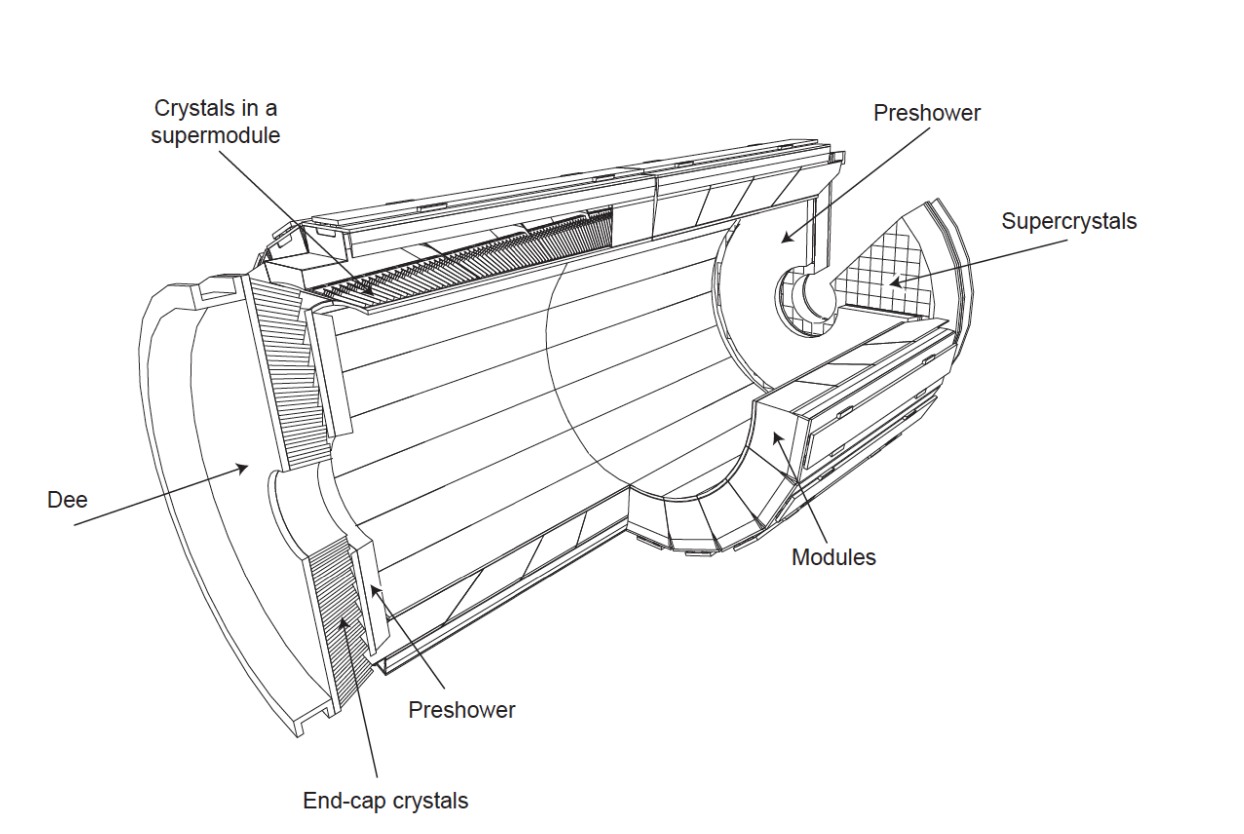
\includegraphics[scale=0.7]{fig/cutawayECAL.png}H
\end{center}
\caption{A cutaway view of the ECAL and its components~\cite{Chatrchyan:2008aa}.
}
\label{fig:cutawayECAL}
\end{figure}


\subsection{HCAL}

The Hadronic Calorimeter (HCAL) is designed to measure the energy of hadrons that are typically contained in jets. Hadronic showers are more complicated than electromagnetic showers, i.e. the cascade of different particles coming from strong interactions with the nuclei contain charged or neutral pions or neutrinos. This fact poses challenges with the energy resolution and providing coverage for missing energy. For these reasons, the HCAL is substantially longer than the ECAL to fully contain the energy of the incident hadrons. 

Due to budgetary and material constraints, the HCAL cannot be made with the same homogeneous calorimeter material like the ECAL is made from. Instead, it is built as a sampling calorimeter with alternating layers of steel and brass absorber plates and plastic scintillator tiles for most sections of the HCAL. The scintillator tiles carries light through wavelength-shifting fibers to photodetectors that convert the light pulses to electric signals. The sum of the light across the entire shower is proportional to the total energy of the incident hadrons. 

The HCAL is comprised of four subdetectors: The HCAL Barrel (HB) the HCAL Endcaps (HE), the HCAL Forward (HF) and the HCAL Outer (HO). The first two cover up to $|\eta| < 3$. Beyond the HE region, a complementary Cherenkov-light-based system called the HF (Forward), extends the coverage up to $|\eta| <5$. Outside of the magnet, the HO system, with coverage of $|\eta| < 1.26$ has additional scintillators that are installed to complement and improve the energy resolution in the HB. 

\begin{figure}[tbp!]
\begin{center}
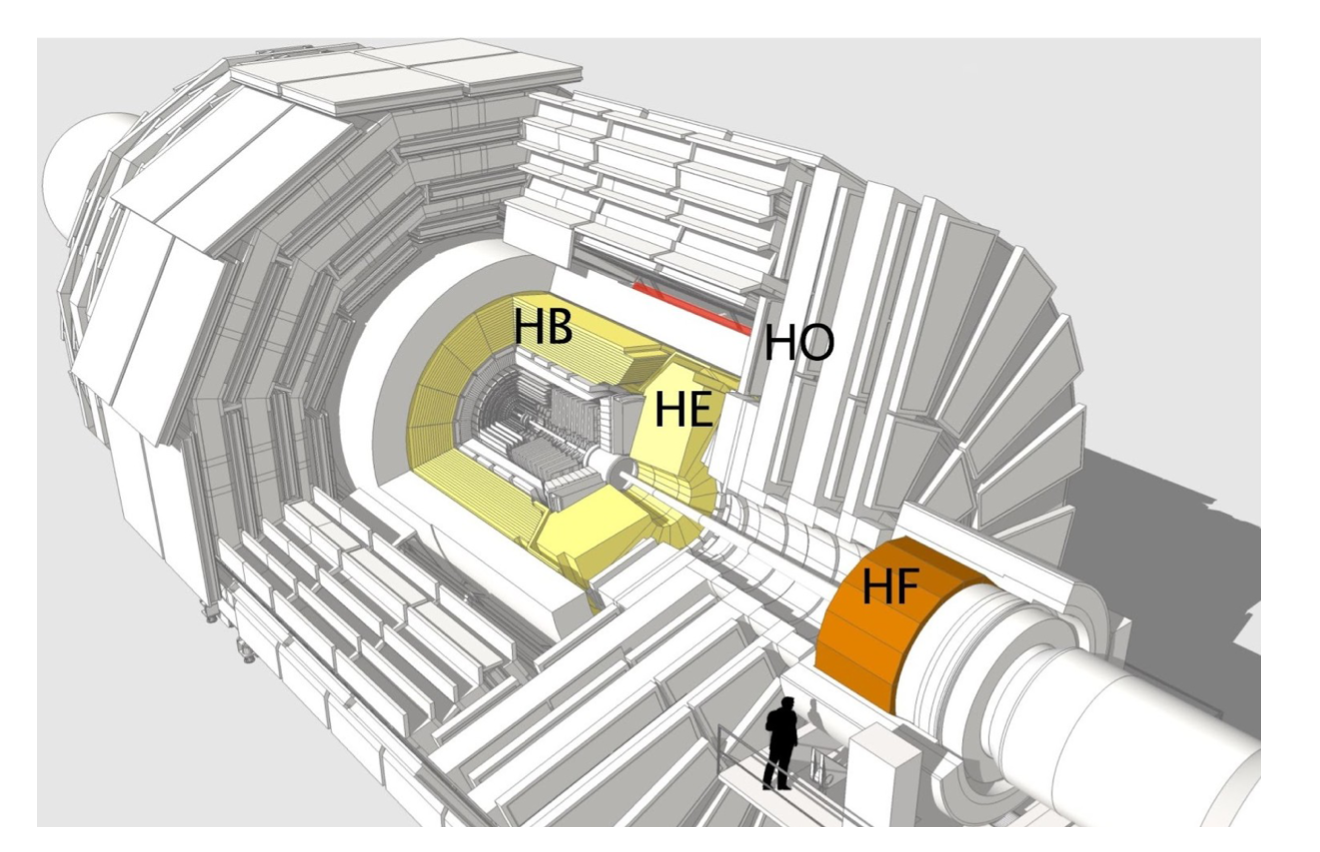
\includegraphics[scale=0.6]{fig/LabelledHCAL.png}
\end{center}
\caption{A cutaway view of the HCAL and its subdetectors~\cite{Chatrchyan:2008aa}
}
\label{fig:HCAL}
\end{figure}


% \begin{figure}[!htb]
% 	\centering
% 	\includegraphics[scale=0.65]{figures/hcal}
% 	\caption{A projection of the HCAL, highlighting its subdetectors~\cite{Chatrchyan:2008aa}.}
% 	\label{hcal}
% \end{figure}

The barrel region of the HCAL consists of the HCAL Barrel (HB) and the HCAL Outer (HO). The HB is situated between the CMS solenoid magnet and the ECAL and spans a radial distance of $1.77 < r < 2.96$ m, with a pseudorapidity coverage $|\eta| < 1.3$. The first layer of the HCAL consists of a plastic scintillator made of 9 mm Bicron BC408 which is different from the succeeding layers of scintillators. This upgrade was made to enhance the depth-segmented readout~\cite{Cummings_phdThesis}} which was made to measure the hadronic showers that began in the ECAL. The information obtained from this layer directly affects our photon identification strategy. The first and last layers of are made of stainless steel absorbers for the purposes of structural support. In between are pairs of brass absorber plates and plastic scintillators. Brass was chosen for cost-effectiveness and robustness against deformation under the strong 4T solenoid field. While these material provide excellent shower containment, the HO was placed behind the solenoid magnet to provide additional detection for the shower tails extending beyond HB. It is made of 10 mm the same scintillator material found behind the ECAL and an additional layer of iron absorber. The HB+HO combination provide an effective thickness of 11.8 nuclear interaction lengths $\lambda_{I}$. Nuclear interaction length is defined as the mean distance travelleld by a hadronic particle before undergoing an inelastic nuclear interaction.

The HCAL endcaps are located between $ 3.9 < |z| < 5.7$ and covers the range $1.3 < |\eta| < 3.0$. As mentioned earlier, the HF extends coverage in the forward region to $|\eta| = 5.2$, located 11.2 m from the detector origin. Instead of plastic scintillators, it uses quartz fibers as the active material to produce Cherenkov light. The forward region experiences the highest particle fluxes in the detector, about 8 times as much as other subdetectors and therefore the switch in material. Steel absorbers are used in the HF. 

The HB+HE region provides a granularity of $\Delta \eta \times \Delta \phi= 0.087 \times 0.087$, a similar coverage of $5\times5$ EB crystals for $|\eta| < 1.6$ while for $|\eta| > 1.6$ the granularity is coarser $\Delta \eta \times \Delta \phi= 0.174 \times 0.174$. Across the depth of a single $\Delta \eta$ region, towers of scintillation light are formed. The plastic scintillators of the towers are connected to wavelength-shifting (WLS) fibres which are routed to hybrid photodiodes (HPD) which are then read out to the electronics for processing. We discuss more on the electronics in later sections.  

In terms of resolution, the HCAL performance is much better evaluated with the jet and $p_T$ resolutions of the ECAL + HCAL system instead of just HCAL alone. The results are similar to that described in Eq.~\ref{eq:energyresolution}.

\subsection{CMS Data Trigger and Electronics }

The LHC proton-proton collisions occur every 25 ns, or 40 MHz. This corresponds to a 1 MB average event size, with 40 PB of data if every event was to be recorded. In one year alone, the data produced by the LHC is around one order of magnitude bigger than the total size of objects ever stored on commercial cloud storage services making the LHC one of the most prominent players in the Big Data era~\cite{Clissa:2021}. The strategy then is to determine in advance only the events that are of interest. CMS does this with a two-level filtering scheme employed to progressively reduce the data collected. The first stage of event rate reduction, called Level 1 (L1) trigger, is performed by high-speed electronics and uses coarser-grained detector information. The event rate is reduced from 40 MHz to about 100 kHz. In the second stage, the high-level trigger (HLT), is software-based menus to further reduce the rate even further from 100 kHz to 2kHz. Unlike L1, HLT uses the full detector granularity, i.e. the information from all the subdetectors including the inner tracks. Only events that pass through both the L1 and HLT are stored for offline physics analysis. Figure~\ref{fig:LHC_BigData} shows how untriggered LHC data compares other Big Data players. 

% \footnote{Overall, high-energy physics events of interest have $p_{T} > 10$ GeV. }

\begin{figure}[tbp!]
\begin{center}
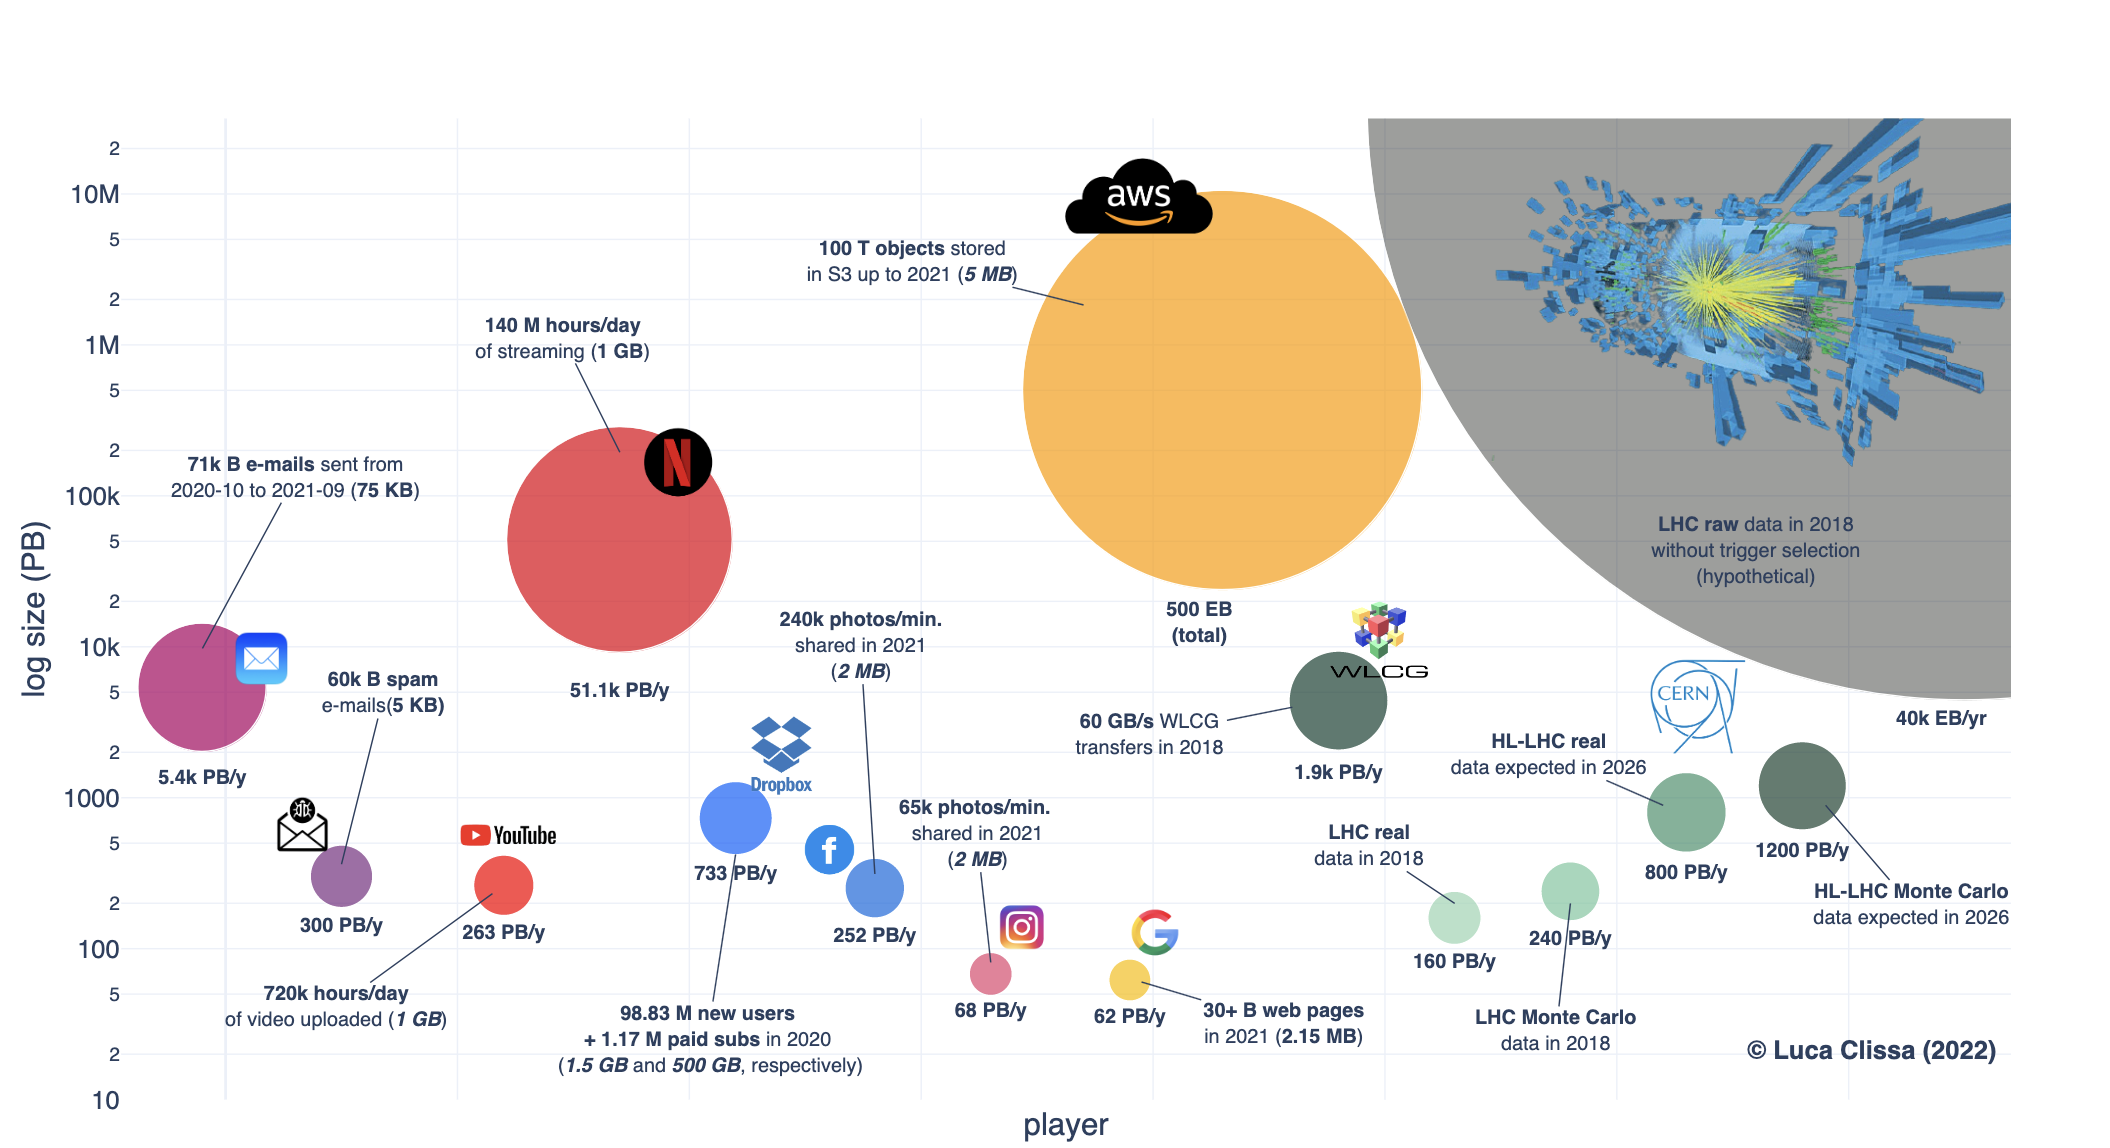
\includegraphics[scale=0.4]{fig/BigData.png}
\end{center}
\caption{An illustration comparing the LHC-produced data without trigger selection to the other Big data players~\cite{Clissa:2021}.
}
\label{fig:LHC_BigData}
\end{figure}


\subsubsection{L1 Trigger}
The L1 Trigger system makes a decision to accept an event within 3.2 $\mu s$, with every single step in the decision-making chain made before the next proton-proton bunch crossing, i.e. within less than 25 ns. This speed of decision-making requires custom-programmed FPGAs or ASICs that are situated in the front-end or what is called on-detector electronics. These hardware are characterized for their radiation tolerance being situated so close to the detector components. 

\begin{figure}[tbp!]
\begin{center}
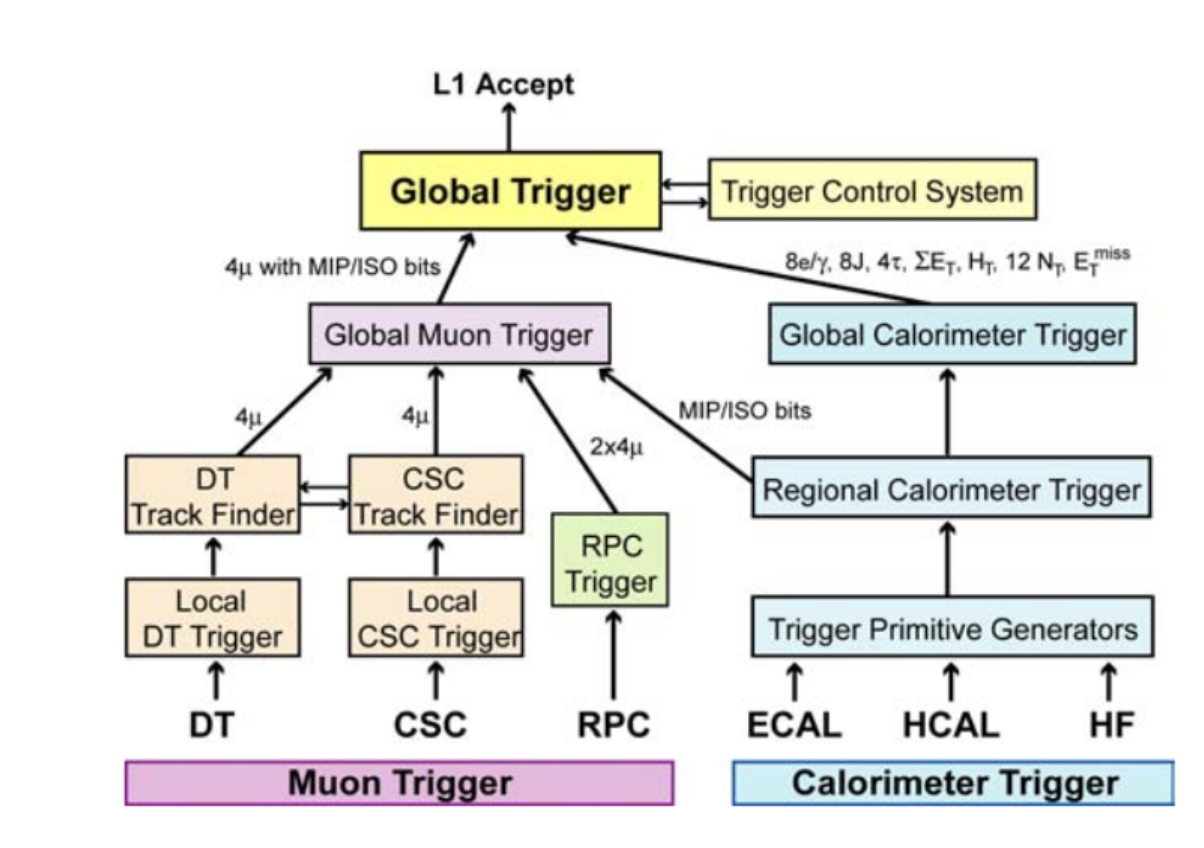
\includegraphics[scale=0.6]{fig/L1Trigger.png}
\end{center}
\caption{A cutaway view of the HCAL and its subdetectors \cite{CMS:2008xjf}
}
\label{fig:L1Trigger}
\end{figure}

The architecture of the L1 system is shown in Figure~\ref{fig:L1Trigger}. An event is ``L1 Accepted" based on aggregated information from the calorimeter and muon systems, both of which are organized into a hierarchy of local, regional and global components. For the Calorimeter Triggers, the first step are the local triggers also known as Trigger Primitive Generators (TPGs) which collect $E_{T}$ deposits from the ECAL or the HCAL trigger towers that have a granularity of $\Delta \eta \times \Delta \phi= 0.087 \times 0.087$. The local TPGs also correct bunch crossing information. In the next step, the TPGs are passed on to the Regional Calorimeter Trigger (RCT) which sums the TPG trigger towers into RCT towers ($4 \times 4$ TPG trigger towers). At this step, crude electromagnetic particle candidates are formed are formed. Finally, a Global Calorimeter Trigger receives the information from the RCT to construct jet candidates, and missing $E_{T}$ candidates and more complex electromagnetic particle candidates. The Muon Trigger has a similar pipeline at L1 begins with information coming from the DT, and CSC muon trackers which provide track hits. The aggregated information is passed on to the Regional Muon Trigger (RMT) which performs track reconstruction. The RPC Trigger information is able to reconstruct complete tracks without any intermediate steps because of its superior timing information. The CSC, DT, and RPC  Trigger Chain are then collectively passed on to the Global Muon Trigger (GMT). The combined Global Muon Trigger (GMT) and Global Calorimeter Triggers (GCT) are then passed on to the Global Trigger which makes the final decision on whether to trigger on the event and pass it on to the HLT.

Events that make it through the HLT must further pass a software-based list of cuts called an HLT menus, to reduce the event rate to 1 kHz. An on-site commercial processing farm of more than 10,000 cores, performs the event reconstruction. In this case, there is more time flexibility with triggering using the full detector granularity. Events that make it through this final step are then recorded for physics analysis. 

The HLT menus consists of a set of simple cuts on single objects or events based on topology. For example, in this analysis, we are interested in events with a two-photon final state. The algorithms used by the HLT are similar to that of the offline Physics Reconstruction which we will discuss in the next chapter. 

\subsection{HCAL Online Software and HCAL Upgrades}

A series of upgrades have been planned for CMS with an eye to prepare the detector for the challenges of the High-Luminosity (HL-LHC) era. The first of the of the series termed Phase 1, in between Run 2 and Run 3, in a period called Long Shutdown (2). In this section we discuss the HCAL Phase I upgrade which was completed in October 2019 in time for Run 3 which was unfortunately pushed later to 2022 due to the COVID-19 pandemic. My contributions to HCAL encompassed upgrades in both HCAL Online Software and both Front-End (FE) and Back-End (BE) Electronics. My major contribution on the HCAL Online Software was work on providing software support for the improved timing information to create an L1 trigger on Long-Lived Particles (LLP), under the supervision of Seth Cooper and Aleko Khukhunaishvilli. I also participated in the refurbishing and accounting of Front-End (FE) and Back-end (BE) electronics which was performed with the team consisting primarily of Grace Cummings, Mary Hadley, Sebastian Yan, Candan Isik and Jay Dittman.

In the first two parts, we first give an overview of the FE and BE electronics in Section~\ref{sec:FEBEHCALElectronics} to guide the reader into the idea behind the L1 trigger on Long-Lived Particles (LLP).

\subsubsection{Front-End and Back-End Electronics}~\label{sec:FEBEHCALElectronics}
The Front-End and Back-End electronics data flow diagram is shown in Figure~\ref{fig:DataFlowHCAL}. The Front-End electronics are composed of units called read-out boxes (RBXs) that contain the following: 4 read out modules or (RMs), 1 calibration unit (CU), Clock, Control and Monitoring Modules (CCMs) and a backplane that connects all the components within an RBX. Each of the RMs cover about a 5 degree division in $\phi$. Each RM is a card pack that has the QIE or charge integration boards and light detectors. The RMs combine light into readout towers and converted into digital data and are transmitted to the back-end electronics. Figure~\ref{fig:ReadOutModules} shows a schematic of the RBXs and Figure~\ref{fig:RBXBurnin904} shows an example RBX set-up at the HCAL test facility at Building 904.

The HCAL Back-end electronics are responsible for receiving the continuous readout information coming from the front-end electronics, calculating and transmitting trigger information, storing and sending the front-end trigger data when a L1-accept has been received from the CMS global trigger~\cite{Cooper:2016kef}. Figure~\ref{fig:DataFlowHCAL} shows a schematic diagram for the backend. It also has a local data acquisition and triggering mode, and also handles fast clock and control signals. Back-end crates are called $\mu$TCA crates which contain an Advanced Mezzanine Card (AMC13) which is responsible for event building and linking the back-end to the CMS central data acquisition (cDAQ) system. The $\mu$HTR performs two functions via the two Xilinx FPGAs. The front FPGA takes input from the front-end data, synchronizes the data and pipelines and calculates and transmits the trigger information. The back FPGA is responsible for buffering and applying zero suppression and transmits data to cDAQ. The upgraded electronics include increased granularity and feature bits based on TDC information which will be relevant in our work on the software support for the HB TDC LUTs. 

I was part of the last phase of the ngCCM refurbishing project and I also helped coordinate the start of the front-end and back-end electronic spares bookkeeping and preparation. The refurbishing of the ngCCMs is largely because of a communication issue loss which was attributed to a manufacturing weakness in the VTRxs. The VTRx optical receivers were found to be temperature-sensitive with temperature increases causing outgassing material to obscure the central part of the optical fibers where light is transmitted~\cite{Cummings:2022kgm}. To mitigate the issue, heat sinks were added within the ngCCMs. 

I also began the preparation of the new AMC13s which were production-tested by Chris Cosby from Boston University. I also updated the firmware to match the latest firmware at P5 which was T1, T2 = $0\times2266$ $0\times34$. As there was not a good criteria as to what would qualify as a good spare, I went through several testing steps such as local event building tests and taking local runs with the new AMC13s loaded in the mock up test area of Bldg. 904 at the CERN Prevessin site. We determined that the final step before swapping them at P5~\footnote{Jay Dittman also proposed that we could swap the five spares with the AMC13s that are known to be working well at P5 so we have 'good hot spares'.} was to do a 904 miniDAQ testing. Local runs do not test cDAQ links. As the miniDAQ software was not well configured before my stay at CERN ended, I delegated the tasks to the rest of the team who would take over the project. Figure~\ref{fig:BackendCrate9041} and Figure~\ref{fig:BackendCrate9042} shows the reworking and testing setups for the AMC13 and ngCCM testing. Credits to Jay Dittman and Grace Cummings for the set-up.

In the first half 2021, I have also participated DAQ On-call and DCS Technical shifts at P5 as well as in the updating of the firmwares for the igloo2 FPGAs in the HF ngCCMs located at the CMS cavern shown in Figure~\ref{fig:HFIglooReprogramming}. 

\begin{figure}[tbp!]
\label{fig:DataFlowHCAL}
\begin{center}
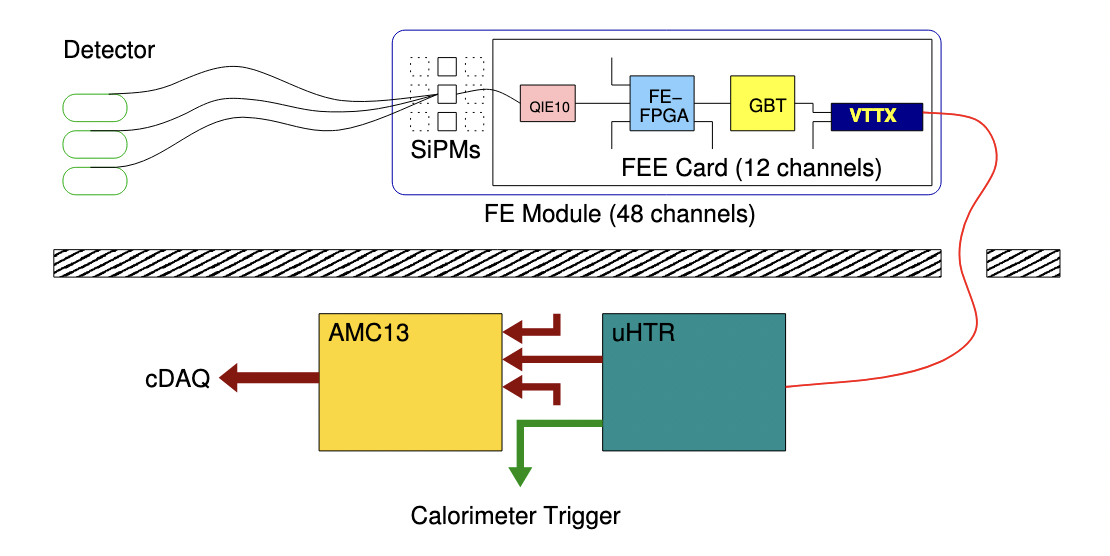
\includegraphics[scale=0.6]{fig/CalorimeterTrigger.png}
\end{center}
\caption{ Schematic diagram of the data flow in HB/HE starting from the photomultipliers through the QIE, FPGA and to the backend and AMC13 and to the CMS DAQ~\cite{Cooper:2016kef}.
}
\end{figure}

\begin{figure}[!htb]
	\centering
	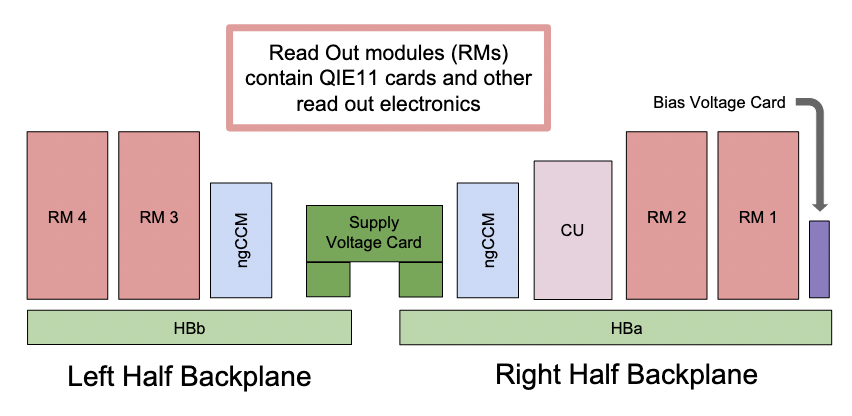
\includegraphics[scale=0.7]{fig/RMs.png}
	\caption{A schematic diagram of an HB RBX containing the 4 RMs, 2 ngCCMs and the backplanes~\cite{Cummings_phdThesis}}
	\label{fig:ReadOutModules}
\end{figure}

\begin{figure}[!htb]
	\centering
	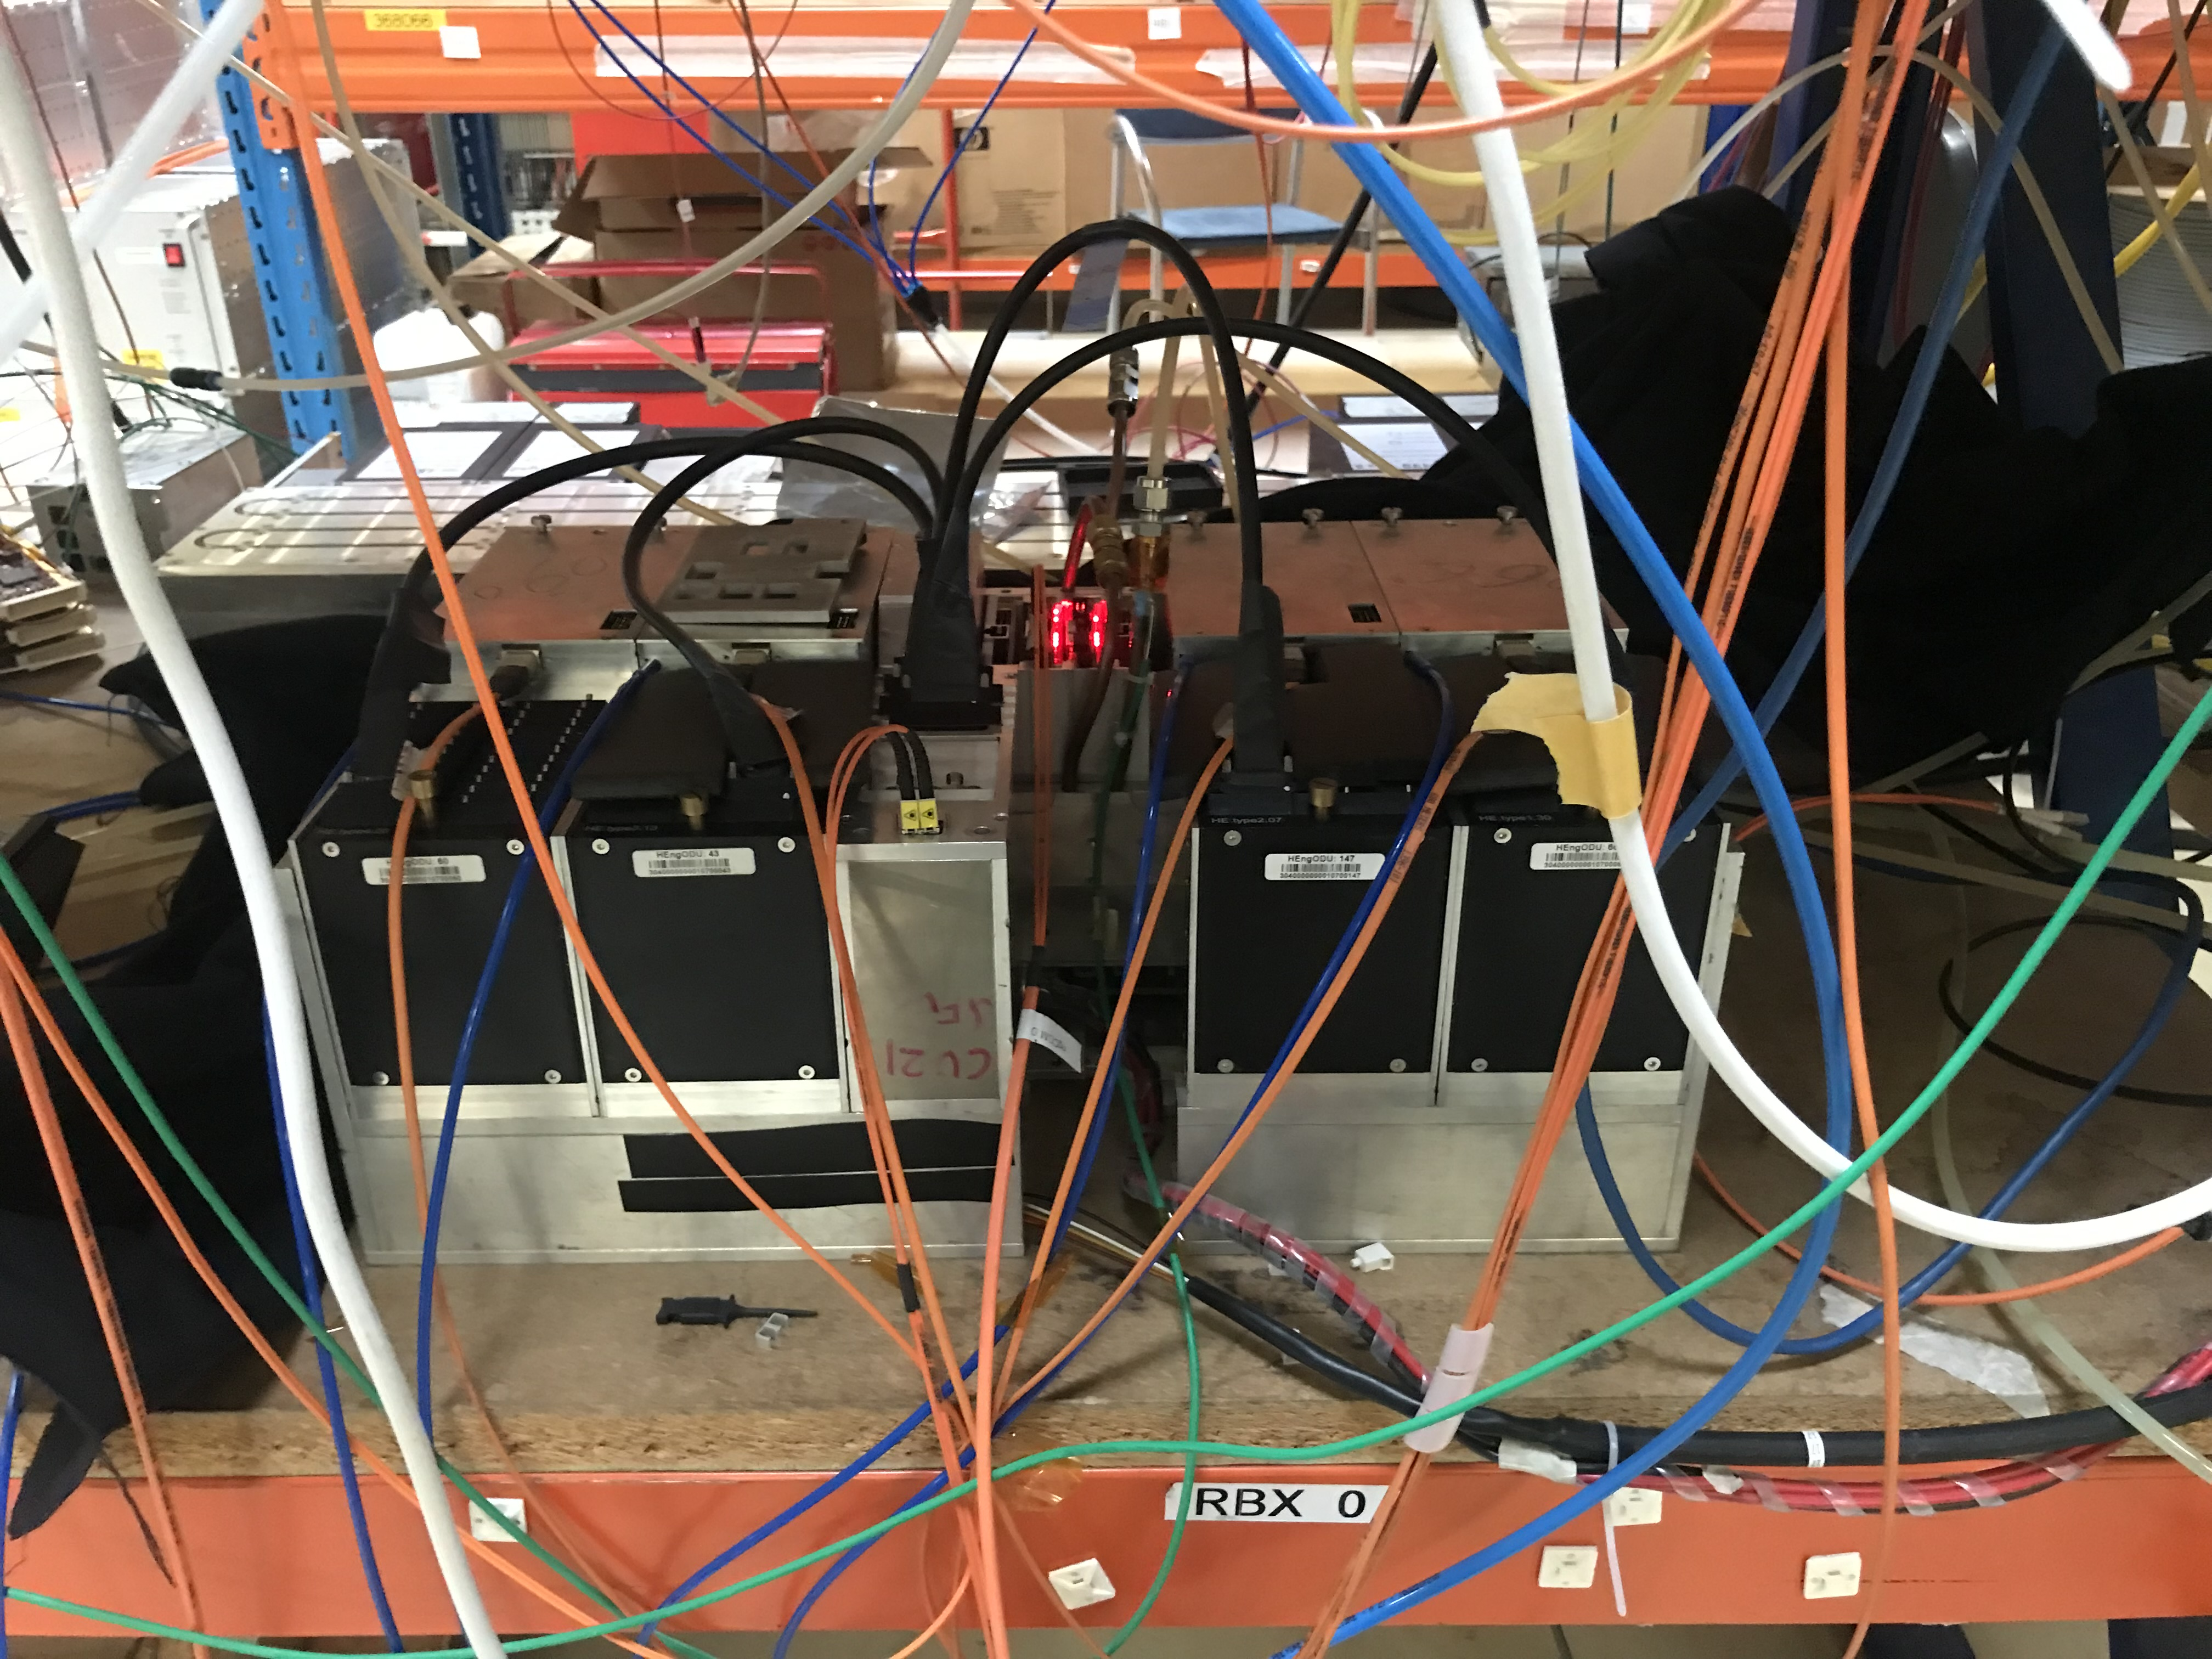
\includegraphics[scale=0.07]{fig/RBXBurn-in.jpg}
	\caption{Image of an RBX at Building 904 where a mock-up of the CMS HCAL Front-End electronics are set up for testing.}
	\label{fig:RBXBurnin904}
\end{figure}

% \begin{figure}[!htb]
% 	\centering
% 	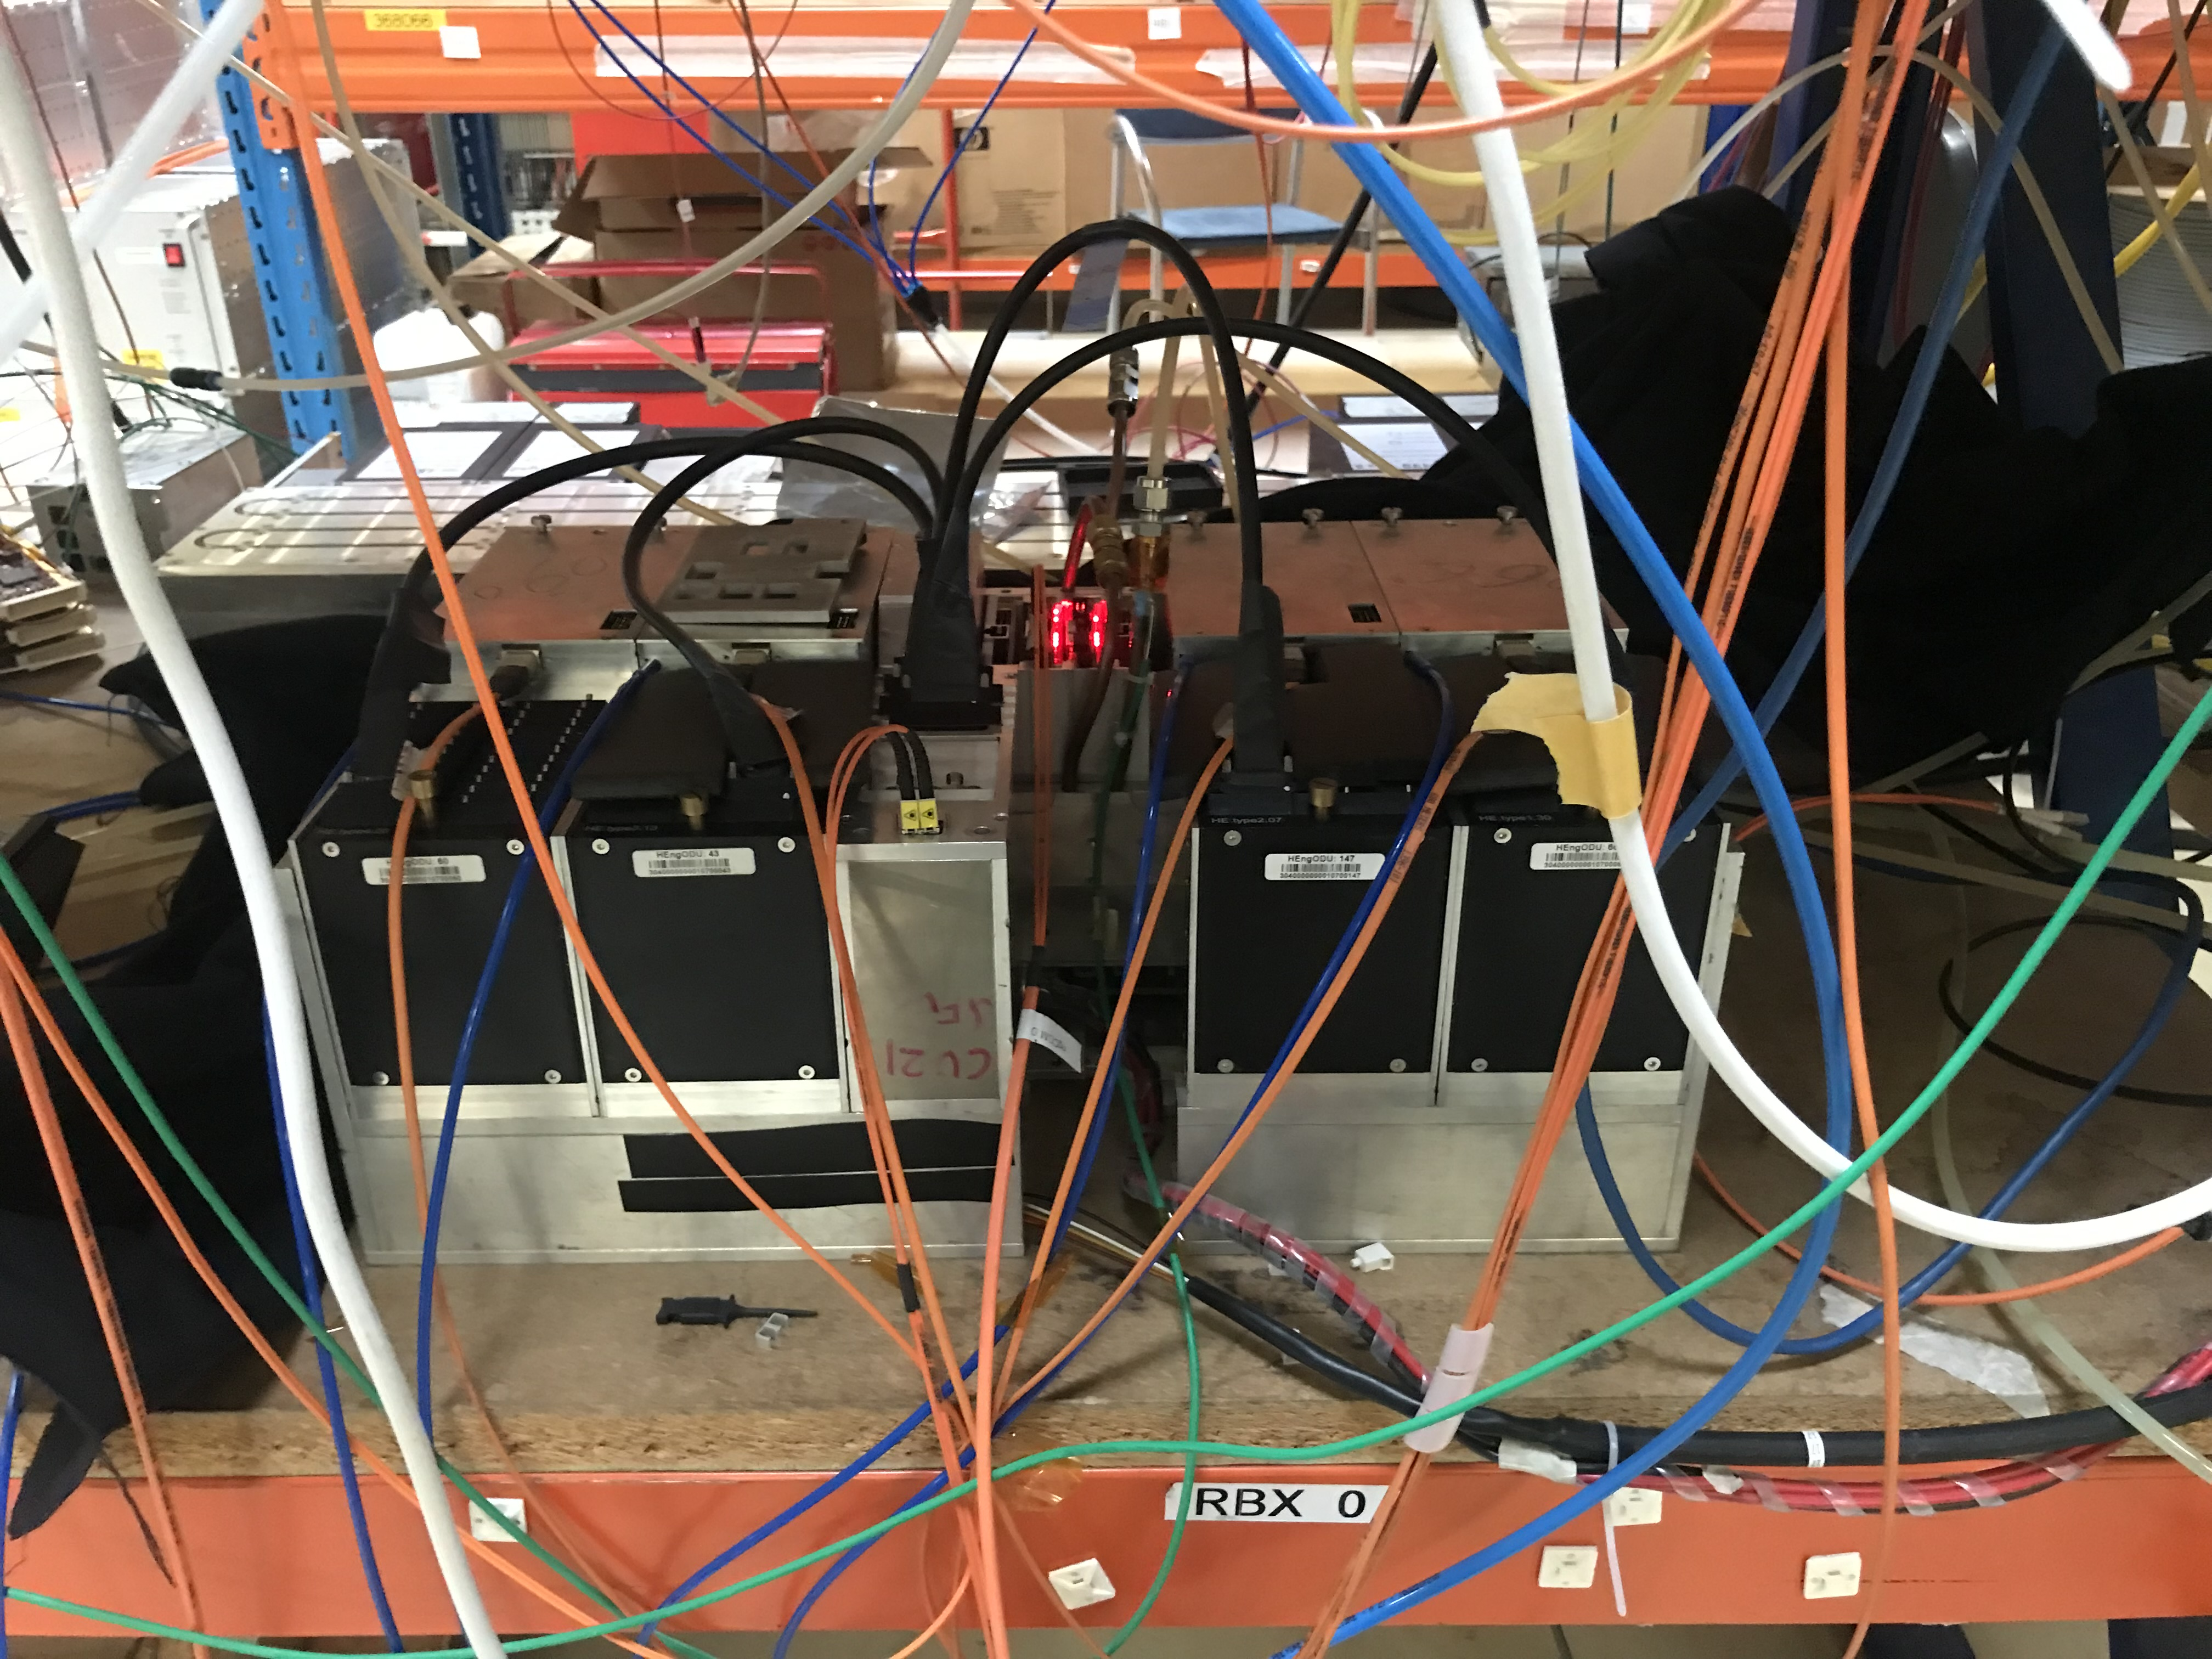
\includegraphics[scale=0.07]{fig/RBXBurn-in.jpg}
% 	\caption{Image of an RBX at Building 904 where a mock-up of the CMS HCAL Front-End electronics are set up for testing.}
% 	\label{fig:BackendCrate904}
% \end{figure}

\begin{figure}[!htb]
	\centering
	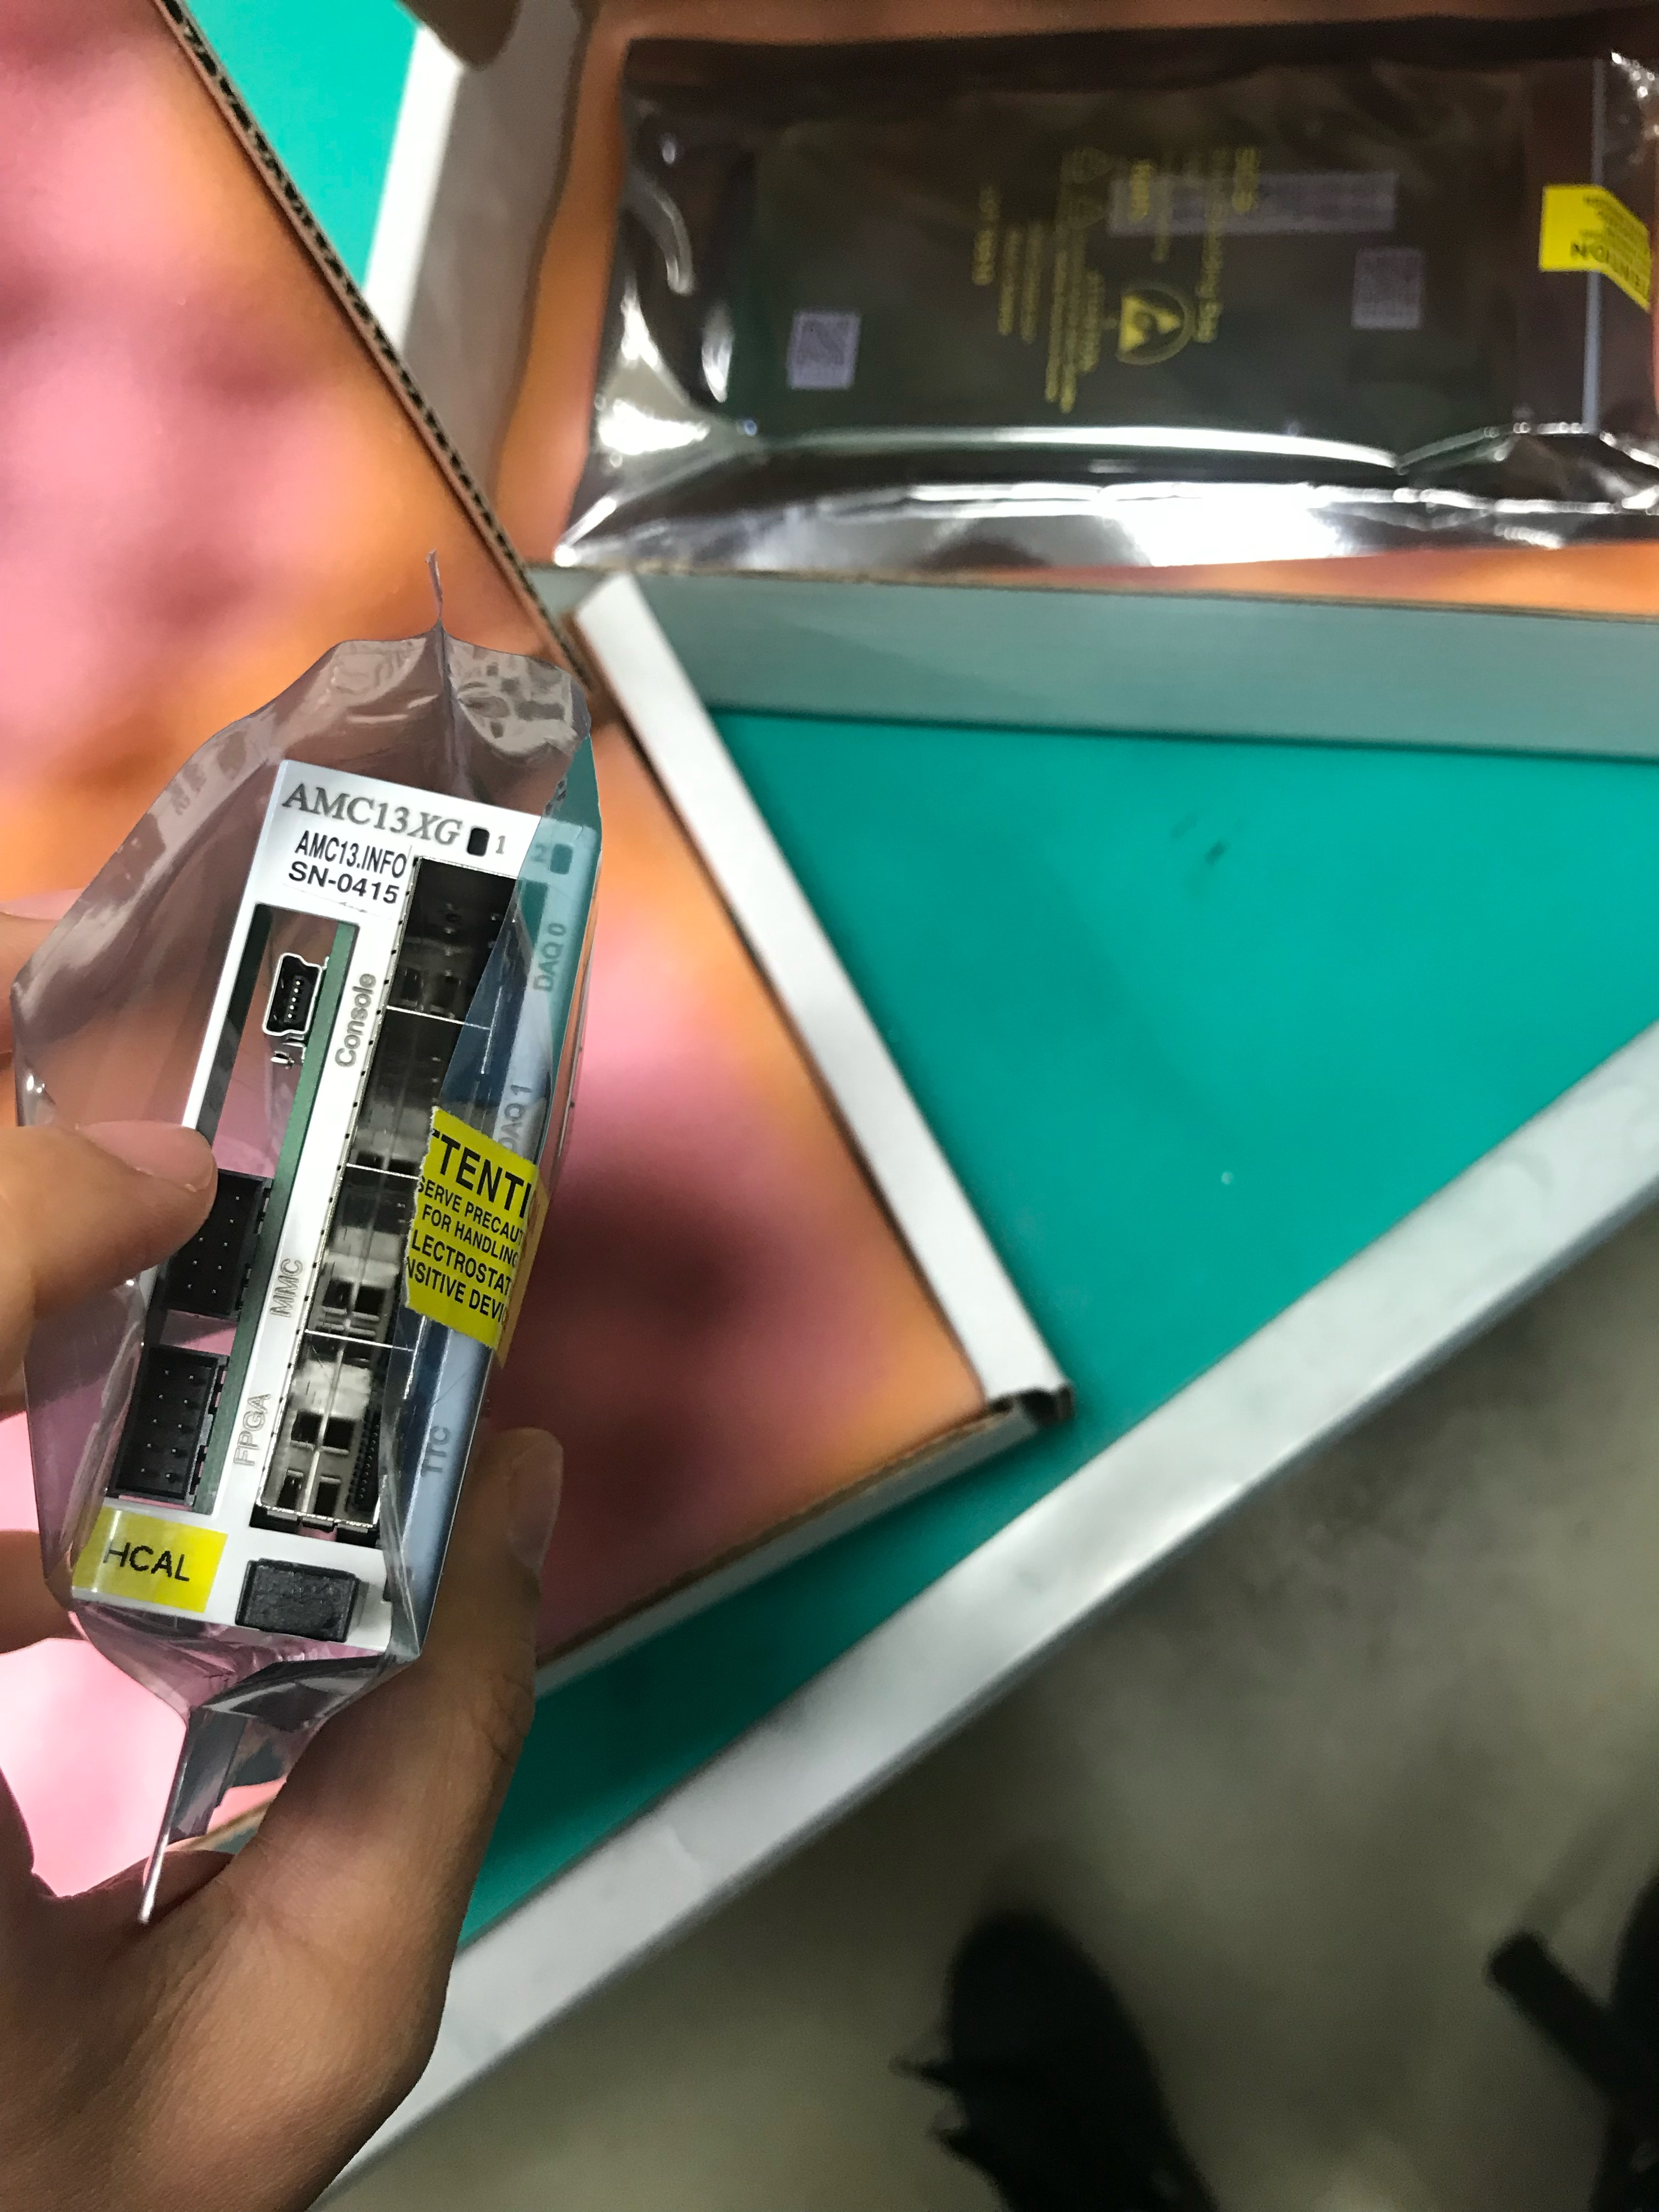
\includegraphics[scale=0.07]{fig/AMC13Reprogramming.jpg}
 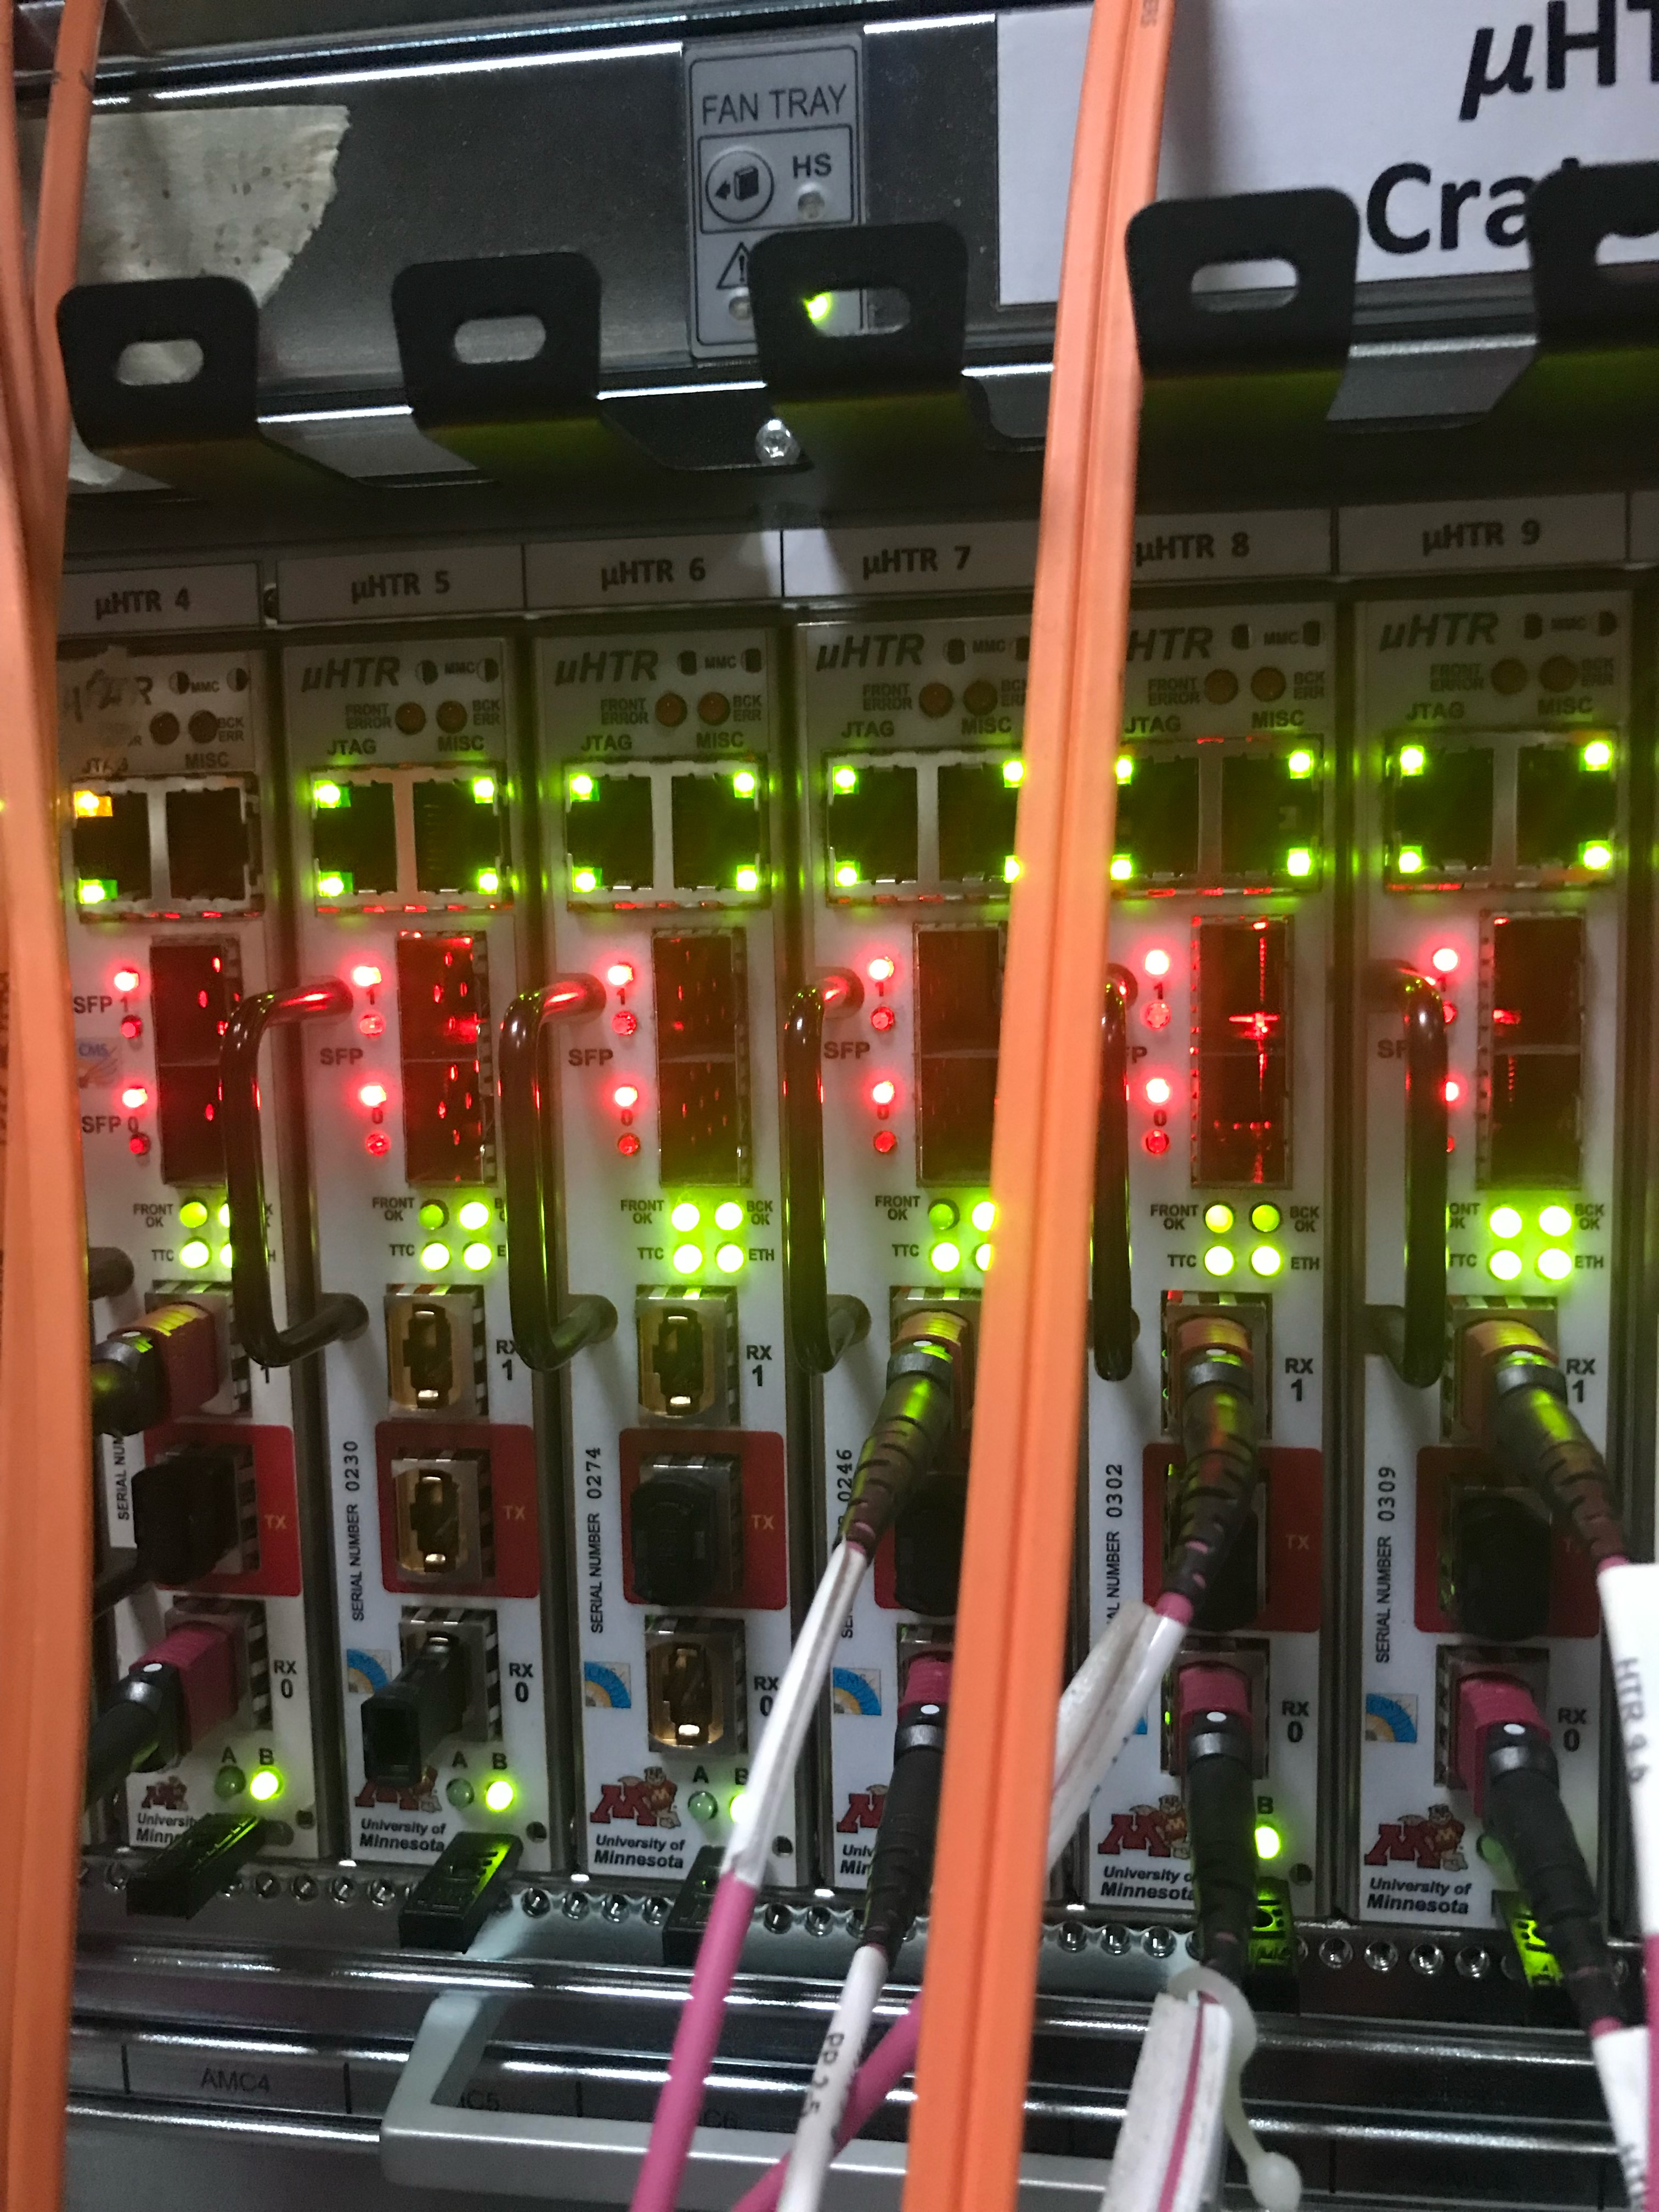
\includegraphics[scale=0.07]{fig/904BE.jpg}
	\caption{On the left is a new AMC13 tested at 904 with the $\mu$HTRs in a selected Back-End Crate shown on the right.}
	\label{fig:BackendCrate9041}
\end{figure}

\begin{figure}[!htb]
	\centering
	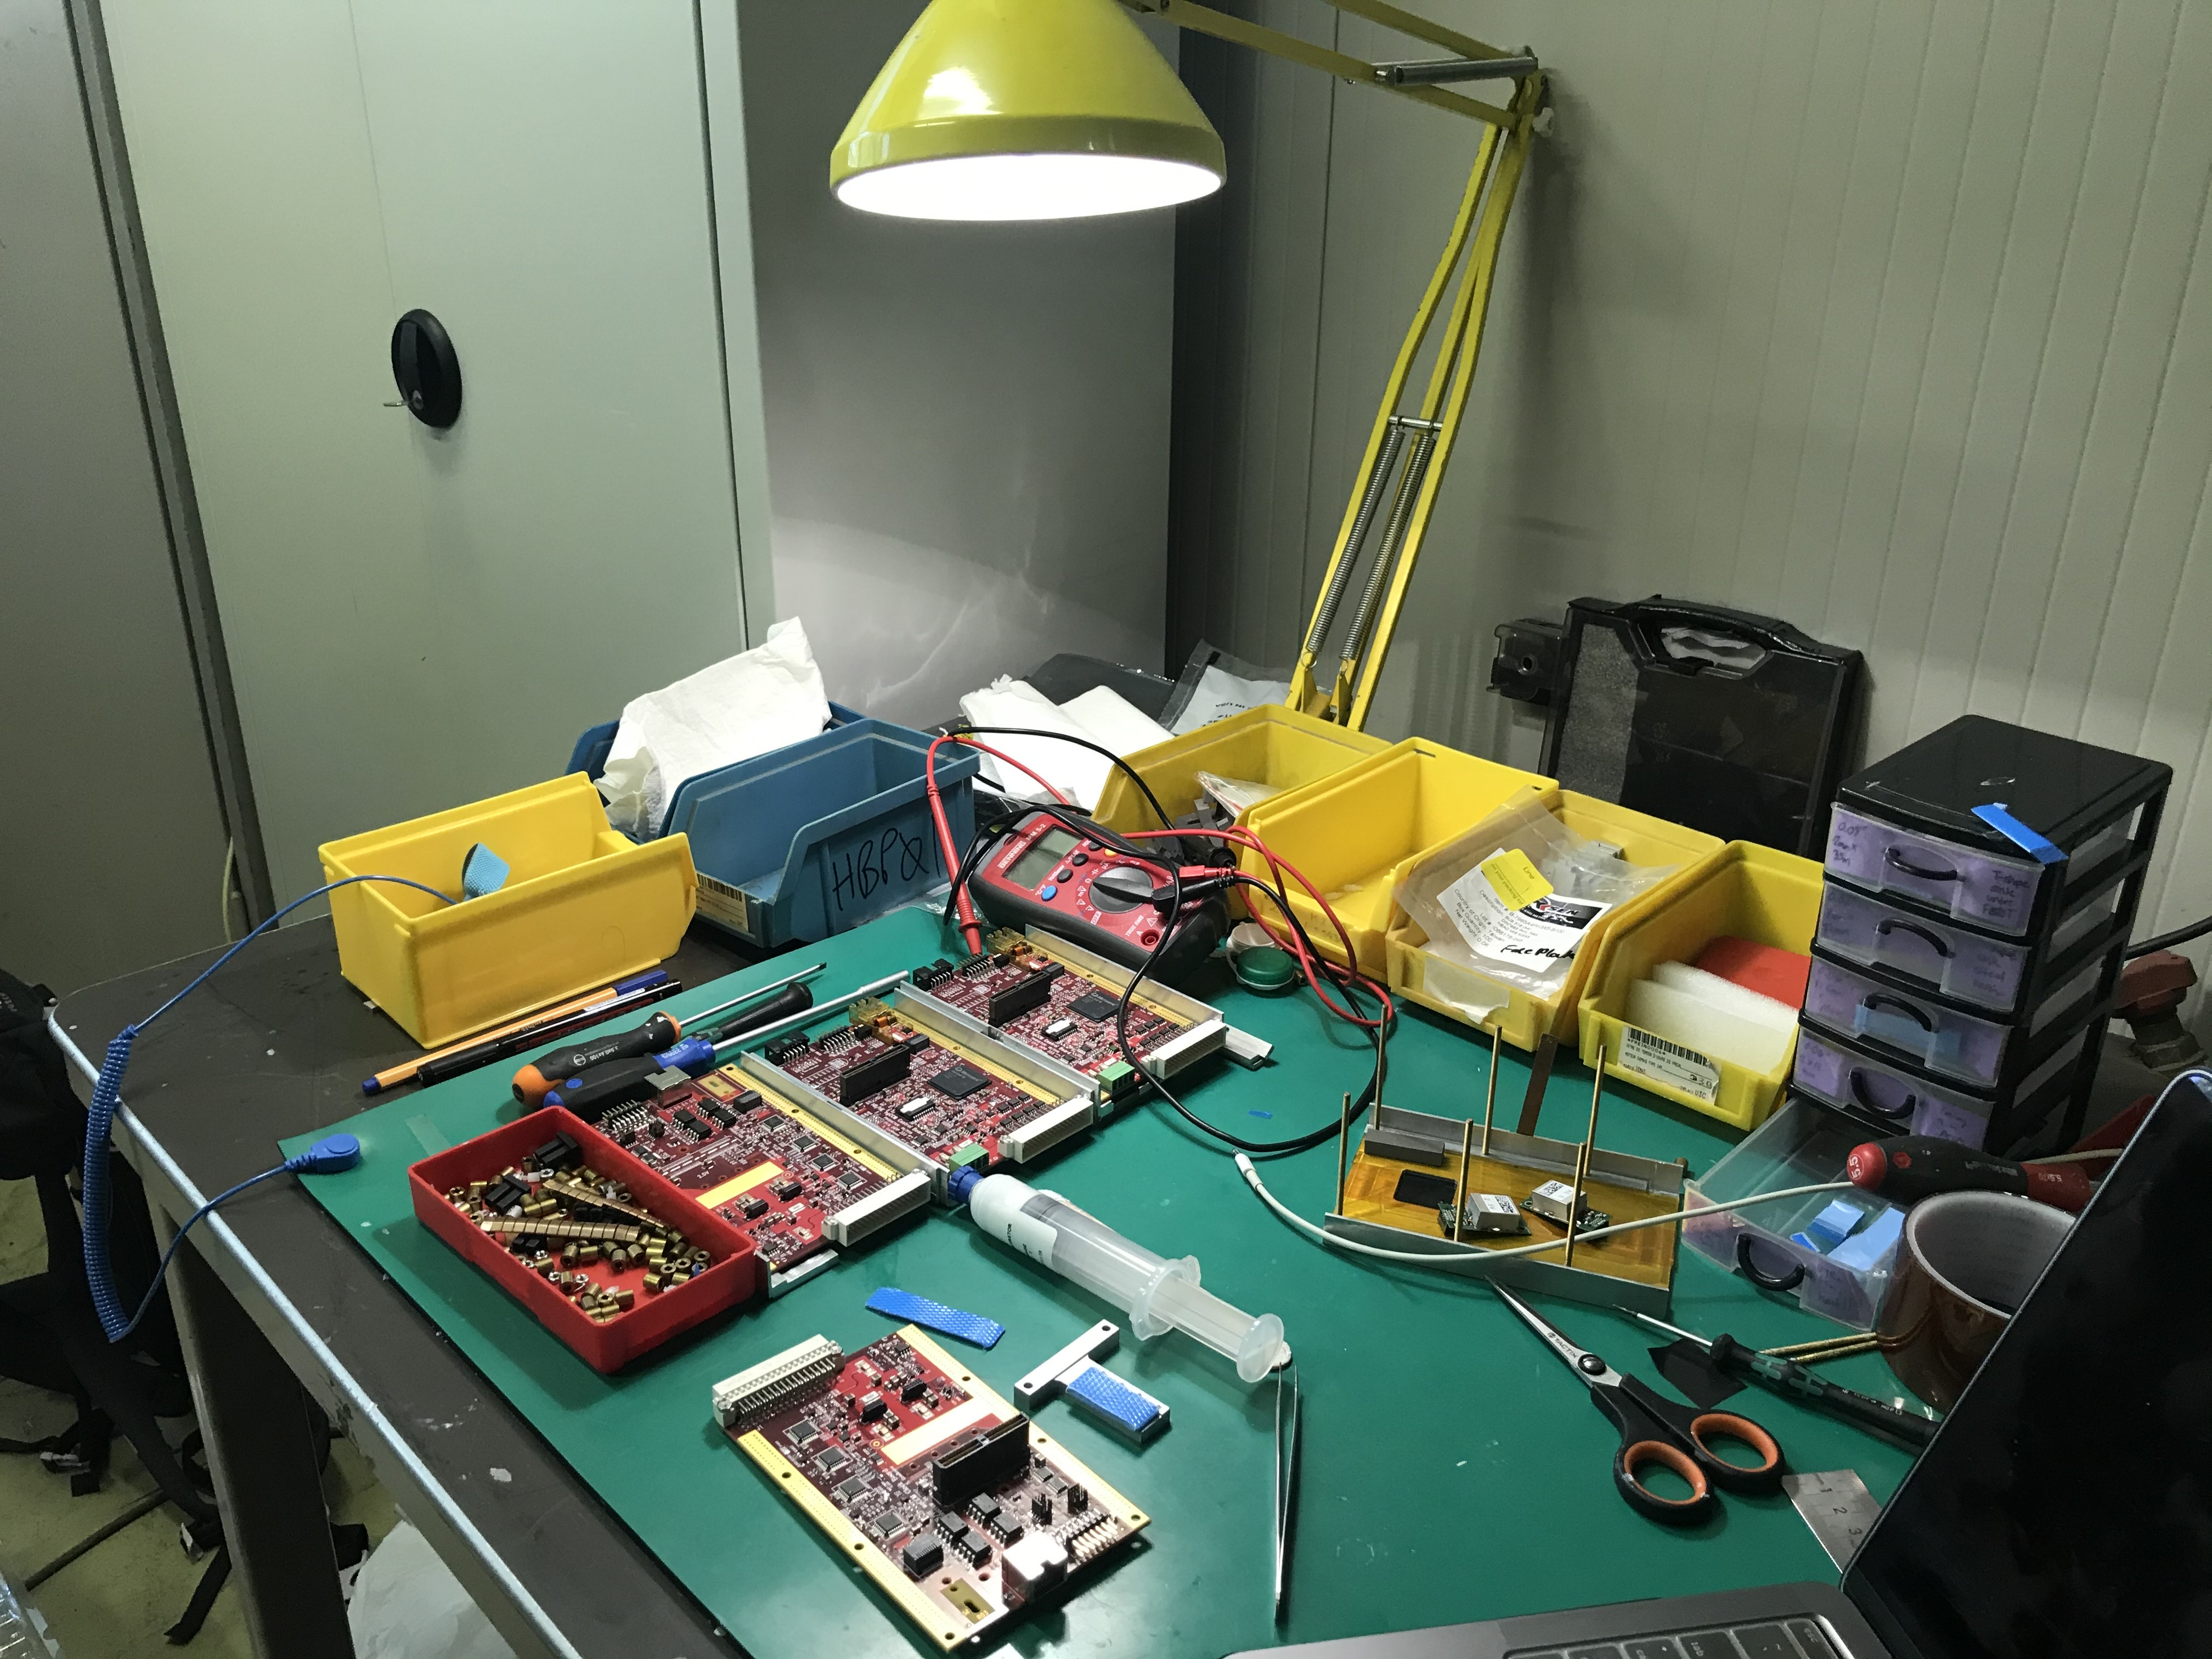
\includegraphics[scale=0.08]{fig/coolingfins.jpg}
     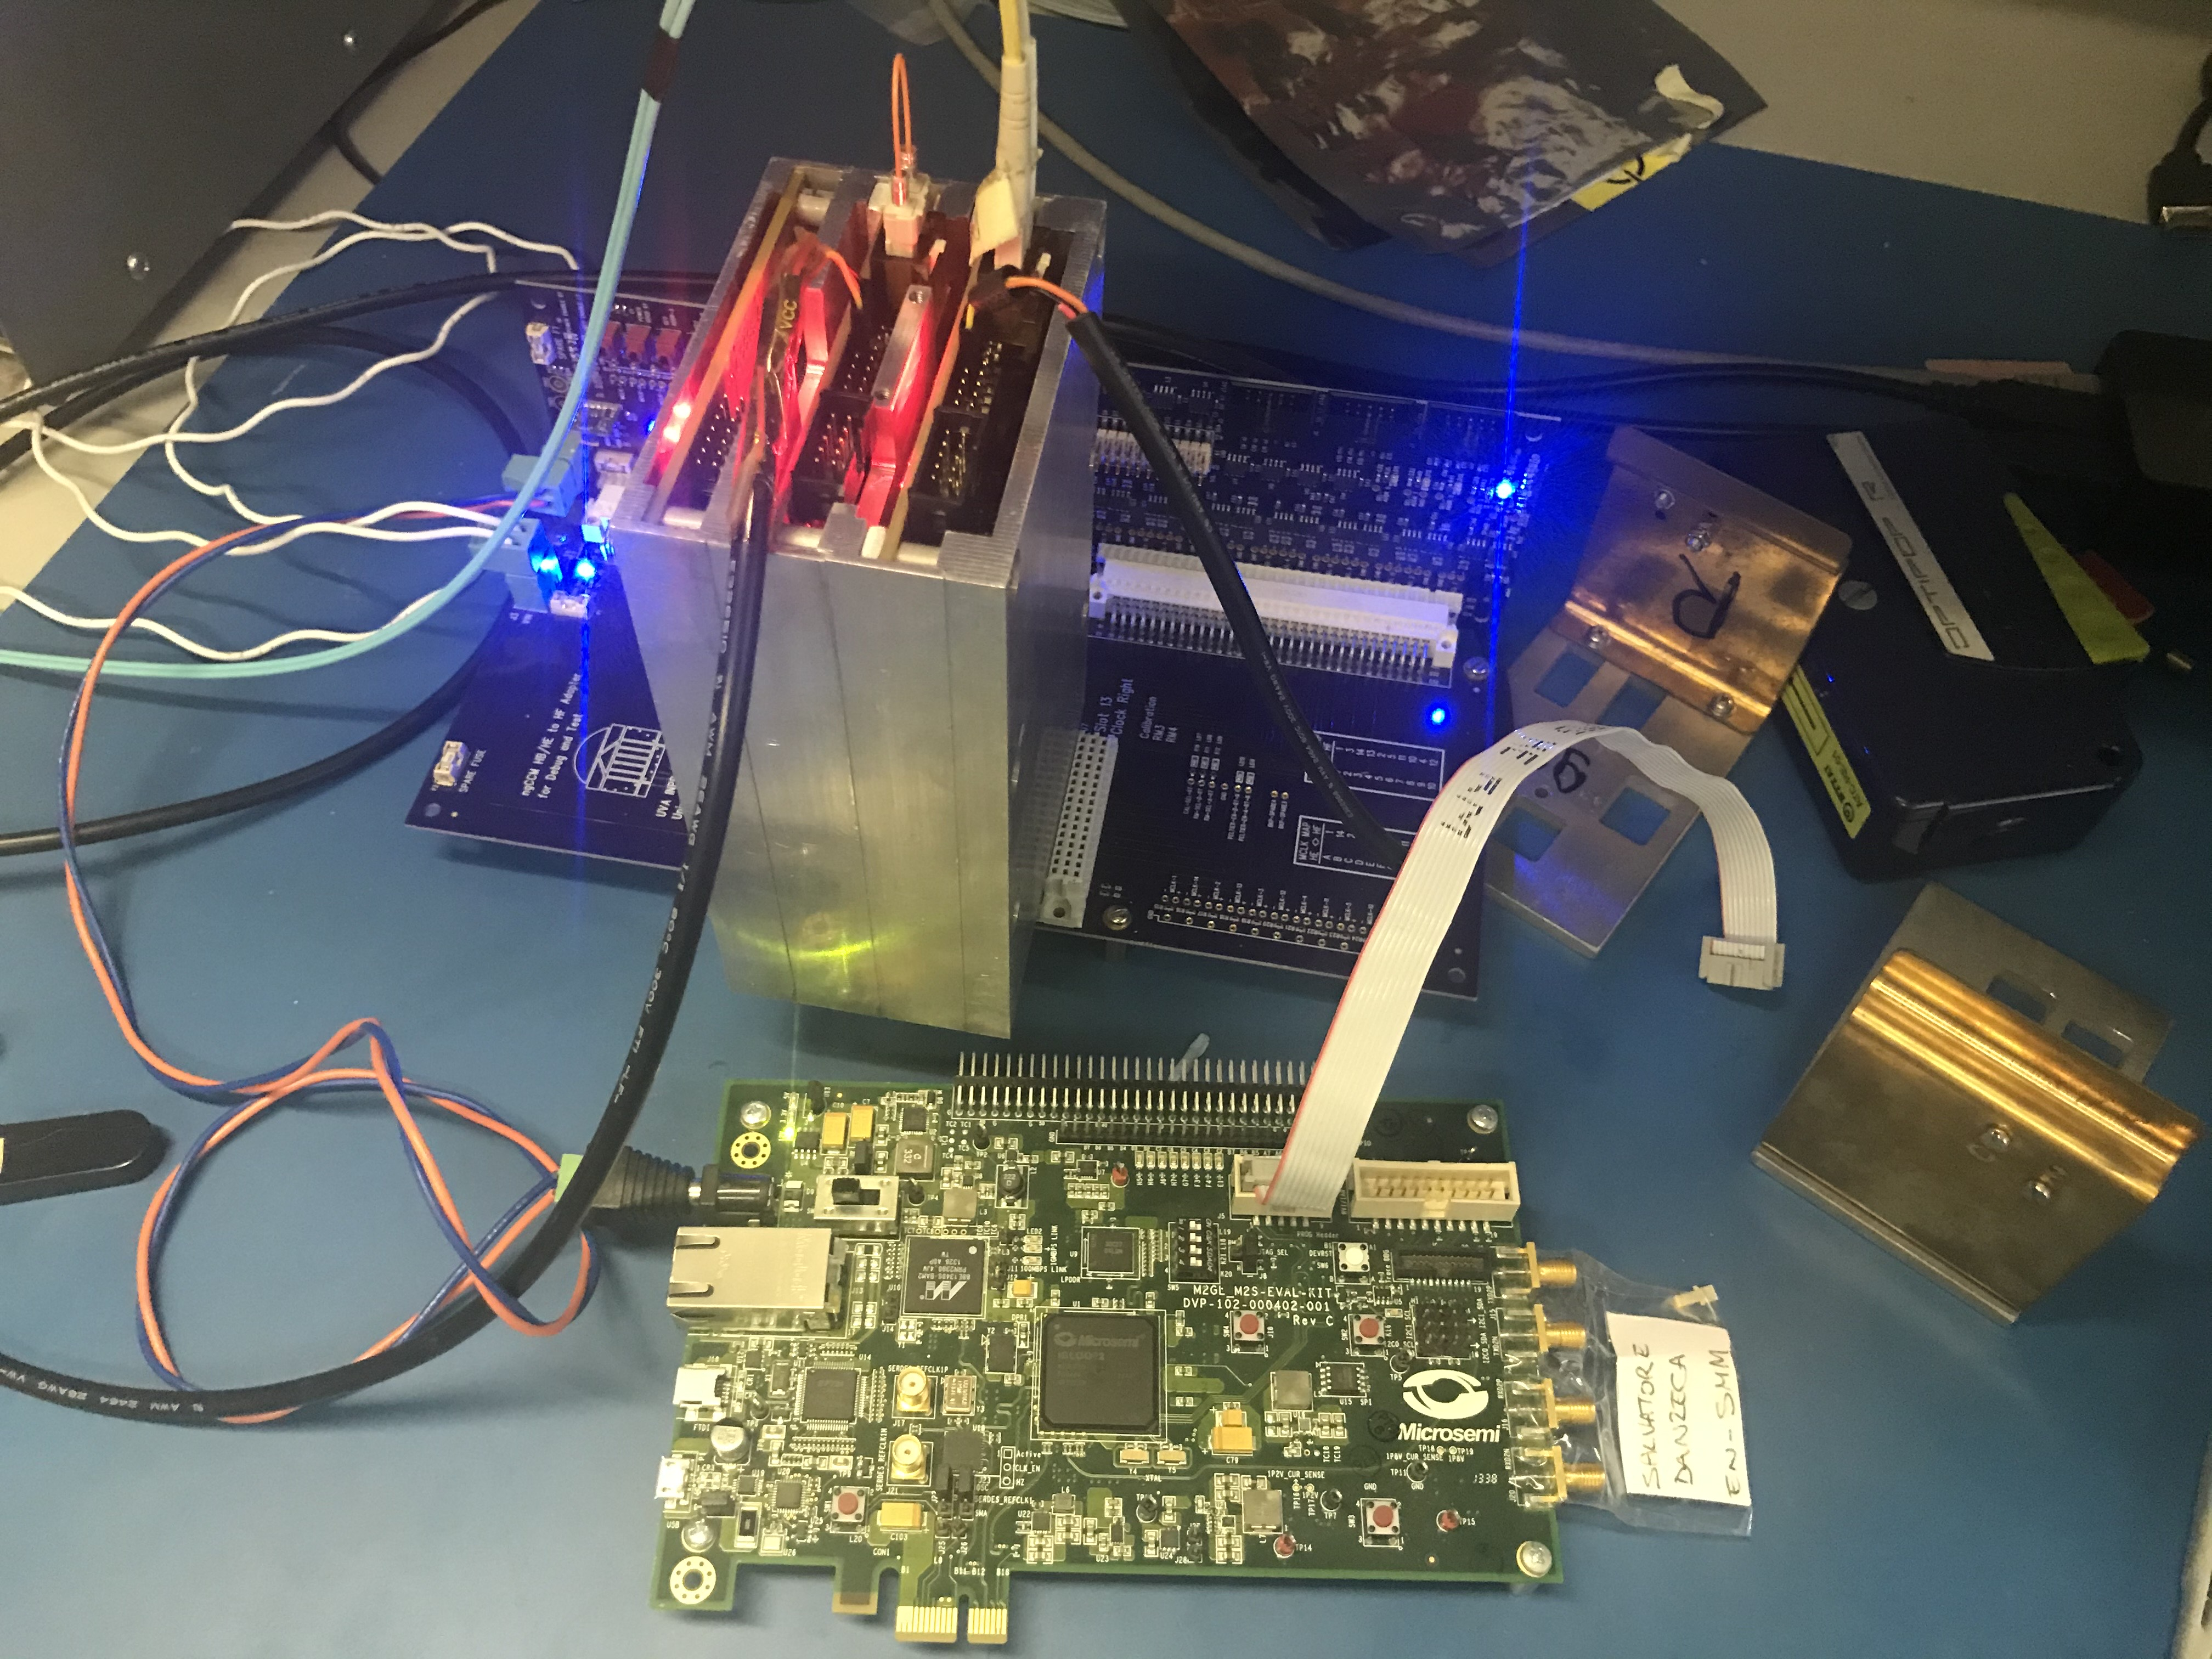
\includegraphics[scale=0.08]{fig/testing.jpg}
	\caption{The top picture shows an ngCCM being reworked to add heat sinks to mitigate the VTRx RSSI drift issue which was related to the communications loss in the HCAL endcap. The right shows a reworked ngCCM being tested on a spare backplane.}
	\label{fig:BackendCrate9042}
\end{figure}

\begin{figure}[!htb]
	\centering
	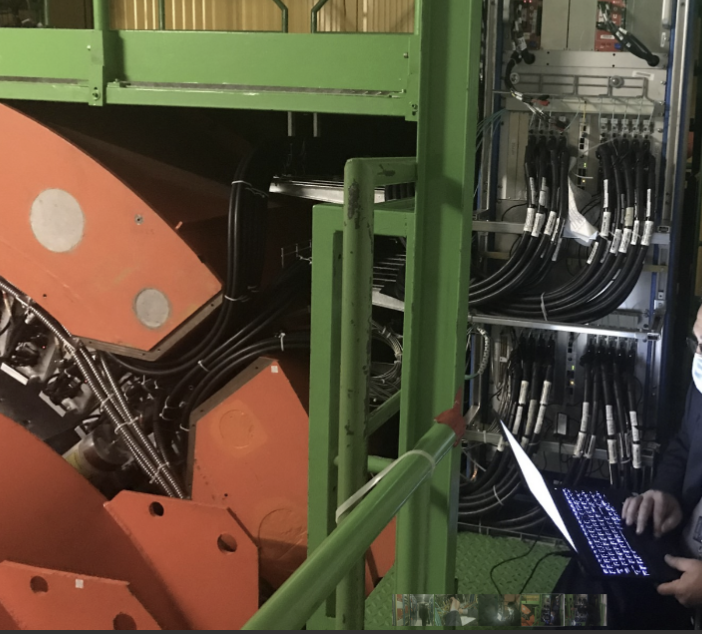
\includegraphics[scale=0.7]{fig/HFIglooReprogramming.png}
	\caption{Reprogramming of the HF Igloo mounted on the HF ngCCMs at the CMS cavern.}
	\label{fig:HFIglooReprogramming}
\end{figure}

\subsubsection{HB TDC LUTs Support for Long-lived Particles}

CMS can take full picture events at 40 MHz but can only record ~1000 full events per second. The idea is to construct a Level-1 (L1) Hardware trigger using the HCAL TDC information within each bunch crossing of 25 ns. Currently, hadronic Long-Lived Particle (LLP) trigger can cover lifetimes greater than ns or microseconds. It is currently at L1 trigger level where the heaviest contstraint lies when it comes to distinguishing prompt particles from long-lived ones. 

\begin{figure}[tbp!]
\begin{center}
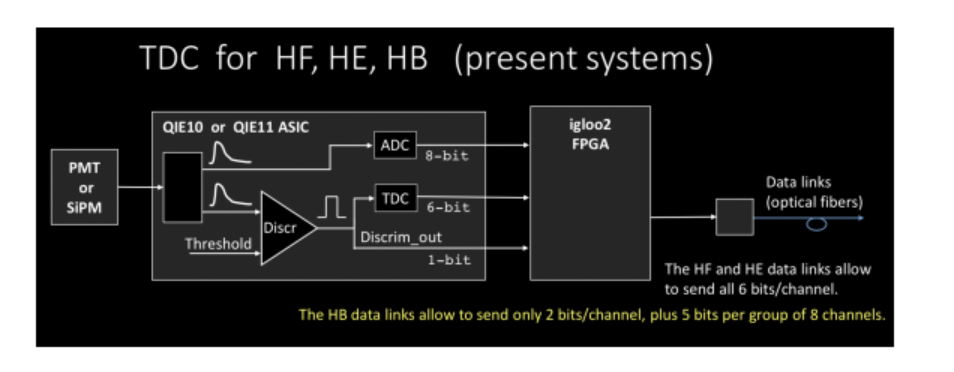
\includegraphics[scale=0.9]{fig/TDCLLP.png}
\end{center}
\caption{TDC Current support Credits: Tullio Grassi}
\label{fig:TDCHBLimits}
\end{figure}

\begin{figure}[tbp!]
\begin{center}
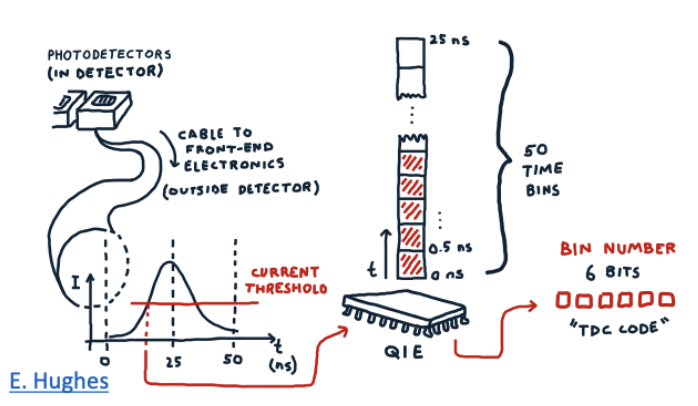
\includegraphics[scale=1.2]{fig/TDCCode.png}
\end{center}
\caption{With the Phase I Upgrade, each QIE channel now has a time-to-digital converter (TDC) which sends out a 6-bit TDC Code. Credit: E.Hughes}
\label{fig:L1TriggerSketch}
\end{figure}

One way to workaround this constraint is to take advantage of the limited bandwidth information. In the HB, only 2 bits/channel are allowed to be sent from the Front-End (FE) electronics to the Back-End (BE) (see Figure~\ref{fig:TDCHBLimits}). This constraint does not exist for both the HE and the HF where the full 6 bit/ channel are transmitted through the data links from FE to the BE. In the Phase I upgrade, each QIE channel now has a time-to-digital converter (TDC), that sends out a 6 bit code.  This is illustrated in a schematics shown in Figure~\ref{fig:L1TriggerSketch}. The Igloo2 FPGAs pack the 6-bit information into meaningful 2-bit information through physics Look-up tables (LUTs). In computer science, Look Up Tables maps keys to some value. In this context, the LUTs map the available TDC codes to the time windows within the bunch crossing of interest. Previously, these LUTs were only hard-coded mappings from the 6-bit to 2-bit information. There are several disadvantages to this. One, the FPGA Igloo2 Firmware would need to be updated each time a new Look Up Table is to be used or investigated. Updating the firmware could be time consuming and also could run into the danger of turning the hardware into ``bricks" when the updating process is interrupted. Not only are the FPGAs expensive to replace, one would also have to wait for a time-window to be able to replace them manually underground. The idea then is to make the LUTs configurable and loadable prior to each data taking run. 

Currently, the software support we implemented for the HB TDC Look Up Tables, takes in xml files. An example xml file containing the LUTs is shown in  Figure~\ref{fig:XMLFile}. They are indexed by RBX, QIE, RM which has a one-to-one map to the detector coordinates indexed by $\eta$, $\phi$, and depth. 

\begin{figure}[tbp!]
\begin{center}
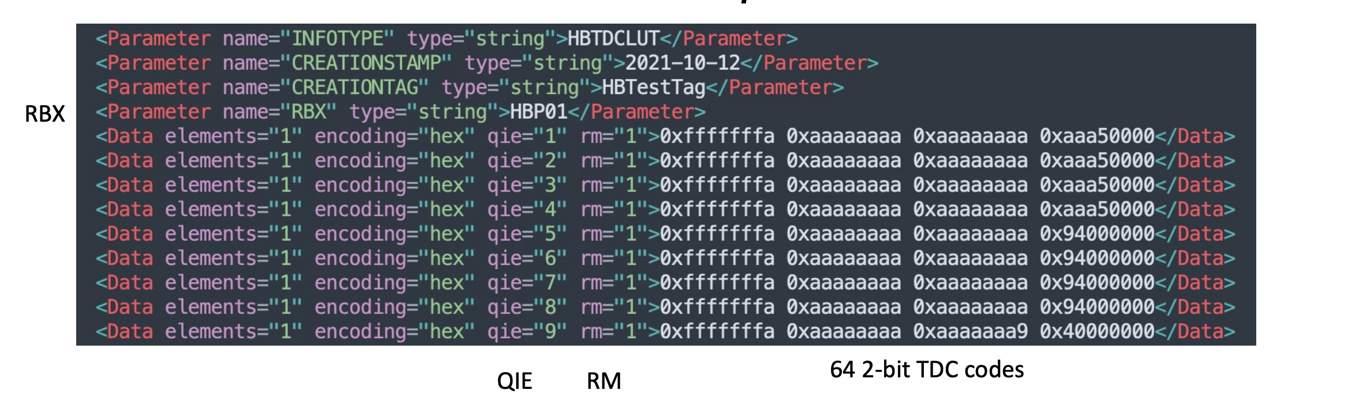
\includegraphics[scale=0.6]{fig/ExampleLUT.png}
\end{center}
\caption{Sample LUT. The RM index ranges from 1-5, where the 5th is the Calibration Unit. Labeling credits: Gillian Kopp}
\label{fig:XMLFile}
\end{figure}

\begin{figure}[tbp!]
\begin{center}
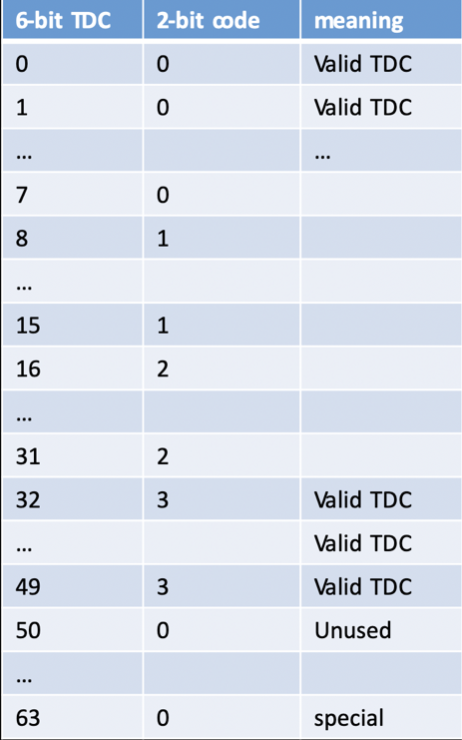
\includegraphics[scale=0.6]{fig/6bitTo2bitMap.png}
\end{center}
\caption{An example of a 6-bit to 2-bit hardmapping information. Credits: Tullio Grassi}
\label{fig:bitMapping}
\end{figure}

An example of a 6-bit to 2-bit mapping as shown in Figure~\ref{fig:bitMapping}. The 6-bit TDC code information comes from the QIE11, which is the processed output of the silicon photomultiplier pulse coming from the detector. Each bunch crossing happens every 25 ns, so the TDC values range from 0-49 in half ns steps to cover the whole time range. Additional error codes are also encoded for example in cases where the pulse starts high (62) or starts low and stays low 
(63).

The 6-bit TDC address from QIE11 is packed into 2-bits in the IGLOO2 firmware LUT, to encode the
following 4 states:

\begin{itemize}
  \item 00 prompt pulse:    $ TDC \leq t_{p}$
  \item 01 slightly delayed pulse: $ t_{p} < TDC \leq t_{p} +2$
  \item 10 very delayed pulse:  $ t_{p} +2 < TDC < 50$
  \item 11 invalid pulse: $ TDC > 50$
\end{itemize}

To determine exactly the time boundary between the states is ascertained from the the distribution of TDC values in a prompt QCD sample and is currently being studies as of time of writing~\cite{HBTDCLUT_uHTR}. One of the potential downsides of loading LUTs was the effect on the configuration time. Prior to every run, the configuration of the various electronics components are set. The new software version was tested at P5 and only an average of 7s was added to the Configuration time. 

% \FIXME{Wishlist: Muon System, References, How the megatiles are grouped together}

% Phase 1 is the system after upgrades installed during Long Shutdown 2 (LS2) of the LHC, between Run 2 and Run 3 of 13 TeV (13.6) TeV running. After the completion of Run 3, the LHC itself will transition to the High Luminosity LHC (HL-LHC). The running conditions of the HL-LHC dramatically differ from those informing the Phase 0 design. Phase 2 upgrades will complete CMS’s preparation for the high luminosity Run 4, and will be installed during Long Shutdown 3 (LS3).
% My work has encompassed almost the entirety of the CMS HCAL Barrel upgrade: the first PCB tests, installation, operations, and finally solving a mystery that ulti- mately impacted a large part of the High Energy Physics community. The following sections describe my contributions to the upgrade effort. First, Section 4.1 intro- duces the HCAL design and upgrade goals. Section 4.2 describes my roles within the HCAL Barrel Upgrade. Finally, Section 4.3 recounts the VTRx (Versatile Link Transmitter/Receiver) failure investigation.

% -------
% Phase I Upgrade of the CMS Hadron Calorimeter
% Seth I. Cooper on behalf of the CMS Collaboration
% Abstract
% In preparation for Run 2 (2015) and Run 3 of the LHC (2019), the CMS hadron calorimeter has begun a series
% of ambitious upgrades. These include new photodetectors in addition to improved front-end and back-end readout
% electronics. In the hadron forward calorimeter, the existing photomultiplier tubes are being replaced with thinner
% window, multi-anode readout models, while in the central region, the hybrid photodiodes will be replaced with silicon
% photomultipliers. The front-end electronics will include high precision timing readout, and the back-end electronics
% will handle the increased data bandwidth. The barrel and endcap longitudinal segmentation will also be increased.
% This report will describe the motivation for the upgrade, its major components, and its current status.

% % https://indico.cern.ch/event/863077/contributions/3850846/attachments/2045904/3427672/llpWorkshop7CMSTriggerV3.pdf


% The Hadron Calorimeter plays an important role in the reconstruction of events in CMS, most notably as the only subdetector capable of measuring neutral hadrons. The hermetic design of the calorimeter allows for the reconstruction of missing trans- verse momentum, a feature that augments HCAL’s existing roles in the calorimeter- based L1-triggers and in electron identification. With the unprecedented luminosity conditions of the HL-LHC on the horizon and the shortcomings of the original front end electronics degrading performance, CMS decided to replace the HCAL front end during the “Phase 1 Upgrade.”
% There are three phases of CMS, each preparing CMS for the next stages of LHC physics. Phase 0 is the originally installed system. 

% In October 2019, the Phase-1 upgrade of the CMS HCAL calorimeter was completed. Each channel now has
% a time-to-digital converter (TDC). The photo-detector technology was changed (hybrid photodiodes were
% replaced with silicon photomultipliers, SiPMs), providing better signal-to-noise performance. In conjunction
% with an increase in the number of readout channels, this allowed a much-improved segmentation in calorime-
% ter depth (longitudinal segmentation). Instead of the previous 1 or 2 (2 or 3) longitudinal readout segments
% in the barrel (endcap) HCAL detector, there are now 4 (up to 7).
% The HCAL trigger is based on the HCAL calorimeter towers. The calorimeter trigger towers in HBHE are
% typically comprised of physical calorimeter towers ganged together in depth. The HCAL trigger primitives
% (TPs) are formed for each trigger tower by combining the information from individual calorimeter towers.
% In addition to the TP generation in HBHE, six “extended bits” of information are also generated that can
% be transmitted to the Level-1 trigger. The meanings of these extended bits (or feature bits) aim to facilitate
% encoding of information about: (i) the longitudinal shower profile data, and (ii) the shower time data
% constructed from the two bits of the TDC information available in each constituent channel of the trigger
% tower. Configurable look-up tables determine which time windows within the BX of interest are represented
% by the available TDC codes. These time window boundaries have a granularity of 0.5 ns. Feature bits as
% determined by the TDC timing or shower profile data can be used to mark hits from late times or from
% distinctive energy deposits in the various layers of the HCAL respectively, that are characteristic of signals
% from long lived exotic particle decays.
% These bits allow the deployment of high efficiency hadronic triggers in Run 3 (and Run 4) operation, and
% are able to capture decays from long lived particles with lifetimes relevant to decays prior to and within the
% HCAL calorimeter volume.








% \section{CMS Experiment - Data Acquisition and Processing}
% The CMS apparatus~\cite{CMS:2008xjf} is a multipurpose, nearly hermetic detector, designed to trigger on~\cite{CMS:2020cmk,CMS:2016ngn} and identify electrons, muons, photons, and (charged and neutral) hadrons~\cite{CMS:2020uim,CMS:2018rym,CMS:2014pgm}. A global "particle-flow" (PF) algorithm~\cite{CMS:2017yfk} aims to reconstruct all individual particles in an event, combining information provided by the all-silicon inner tracker and by the crystal electromagnetic and brass-scintillator hadron calorimeters, operating inside a 3.8\unit{T} superconducting solenoid, with data from the gas-ionization muon detectors embedded in the flux-return yoke outside the solenoid. The reconstructed particles are used to build \PGt leptons, jets, and missing transverse momentum~\cite{CMS:2018jrd,CMS:2016lmd,CMS:2019ctu}. 

% The central feature of the CMS apparatus is a superconducting solenoid of 6\unit{m} internal diameter, providing a magnetic field of 3.8\unit{T}. Within the solenoid volume are a silicon pixel and strip tracker, a lead tungstate crystal electromagnetic calorimeter (ECAL), and a brass and scintillator hadron calorimeter (HCAL), each composed of a barrel and two endcap sections. Forward calorimeters extend the pseudorapidity coverage provided by the barrel and endcap detectors. Muons are measured in gas-ionization detectors embedded in the steel flux-return yoke outside the solenoid. A more detailed description of the CMS detector, together with a definition of the coordinate system used and the relevant kinematic variables, can be found in Ref.~\cite{CMS:2008xjf}. 

% \subsection{Trigger}
% Events of interest are selected using a two-tiered trigger system. The first level (L1), composed of custom hardware processors, uses information from the calorimeters and muon detectors to select events at a rate of around 100\unit{kHz} within a fixed latency of about 4\mus~\cite{CMS:2020cmk}. The second level, known as the high-level trigger (HLT), consists of a farm of processors running a version of the full event reconstruction software optimized for fast processing, and reduces the event rate to around 1\unit{kHz} before data storage~\cite{CMS:2016ngn}. 

% \subsection{Offline Analysis}
% \section{CMS HCAL Online Software and Electronics}
% Upgrade \cite{Cooper:2016kef}
% VTRX communications loss \cite{Cummings:2022kgm}

% The total integrated luminosity of Run 2 is known with a better relative uncertainty than that of the partial data taking periods. Here is a sentence that could be used in standard papers:

% The integrated luminosities for the 2016, 2017, and 2018 data-taking years have 1.2--2.5\% individual uncertainties~\cite{CMS-LUM-17-003,CMS-PAS-LUM-17-004,CMS-PAS-LUM-18-002}, while the overall uncertainty for the 2016--2018 period is 1.6\%.

% In case the 2015 data is included in the analysis, the sentence above should mention "2015--2018", everything else remaining identical.

% Physics coordination would like to see a citation to the paper CMS-LUM-17-003 in all CMS papers. The BibTeX for the other two PASes is also given below. 


% \begin{figure}[!htb]
% 	\centering
% 	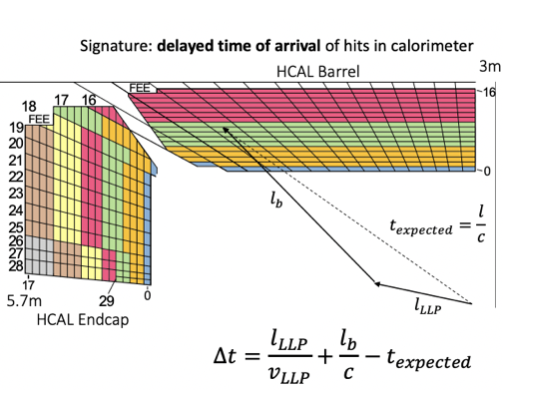
\includegraphics[scale=0.7]{fig/TimeDelay.png}
% 	\caption{An overview of the location of LHC and its four interaction points~\cite{Mouche:1708847}.}
% 	\label{lhc-overview}
% \end{figure}


% \begin{figure}[!htb]
% 	\centering
% 	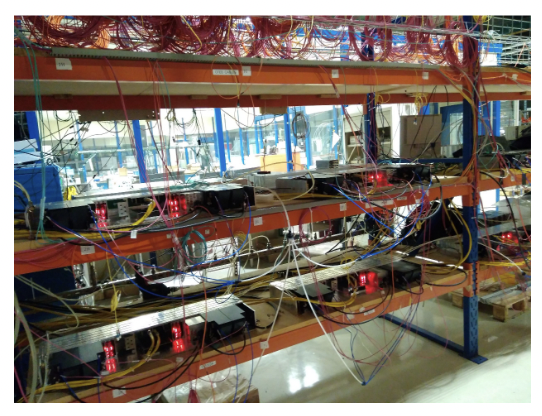
\includegraphics[scale=0.7]{fig/Backend.png}
% 	\caption{An overview of the location of LHC and its four interaction points~\cite{Mouche:1708847}.}
% 	\label{lhc-overview}
% \end{figure}

% \begin{figure}[!htb]
% 	\centering
% 	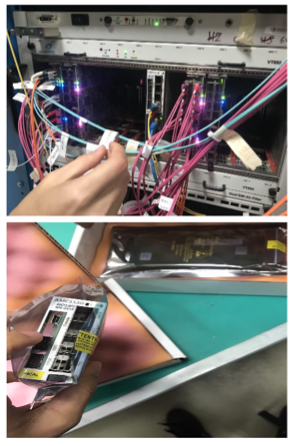
\includegraphics[scale=0.3]{fig/BackEndAMC13.png}
% 	\caption{An overview of the location of LHC and its four interaction points~\cite{Mouche:1708847}.}
% 	\label{lhc-overview}
% \end{figure}

% \begin{figure}[!htb]
% 	\centering
% 	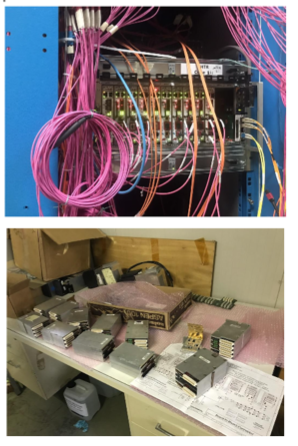
\includegraphics[scale=0.3]{fig/BackendFE.png}
% 	\caption{An overview of the location of LHC and its four interaction points~\cite{Mouche:1708847}.}
% 	\label{lhc-overview}
% \end{figure}

% \begin{figure}[!htb]
% 	\centering
% 	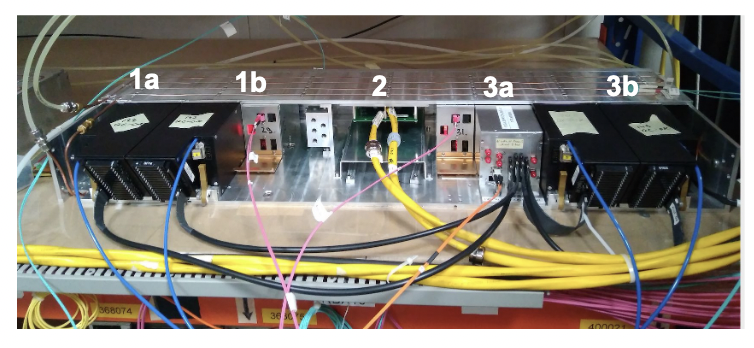
\includegraphics[scale=0.3]{fig/BackendRMs.png}
% 	\caption{An overview of the location of LHC and its four interaction points~\cite{Mouche:1708847}.}
% 	\label{lhc-overview}
% \end{figure}


% \begin{figure}[!htb]
% 	\centering
% 	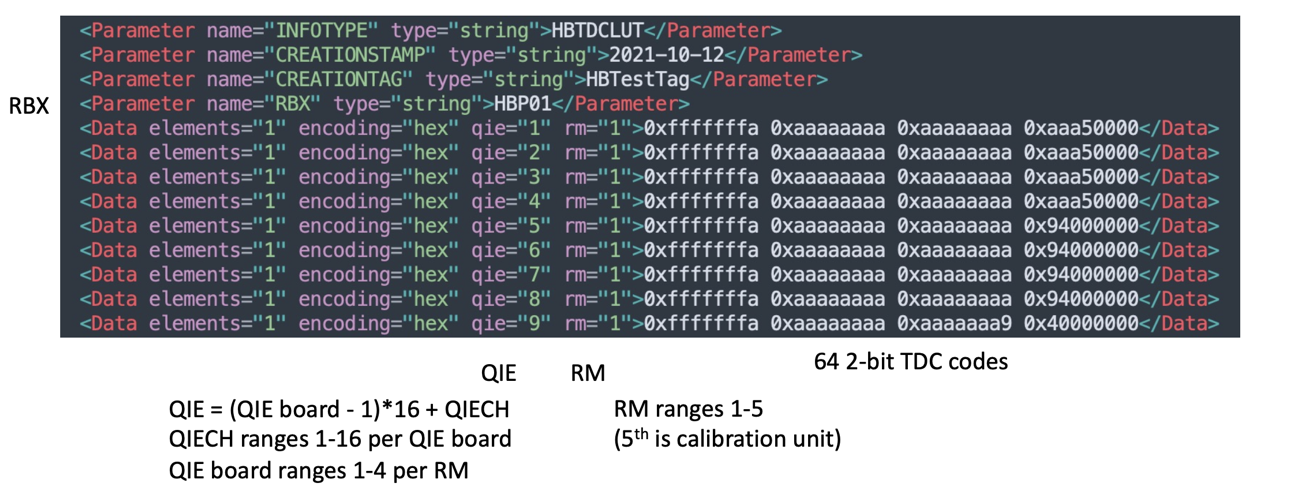
\includegraphics[scale=0.3]{fig/RBX_RM_QIE.png}
% 	\caption{An overview of the location of LHC and its four interaction points~\cite{Mouche:1708847}.}
% 	\label{lhc-overview}
% \end{figure}



        
\newpage
% \section{References}
% \renewcommand{\bibsection}{}%removes the spaces and unwanted references heading from the list
% \begin{singlespacing}
% \bibliographystyle{apsrev}
% \bibliography{Ref_LHC_CMS.bib}
% \end{singlespacing}\par
% %{\let\thefootnote\relax\footnote{{Copyright: \copyright 2019 Elsevier B.V.}}}
